%*******************************************************************************
%****************************** Third Chapter *********************************
%*******************************************************************************

\chapter{Inhomogeneous Electroluminescence in InGaN QW LEDs}

\ifpdf
    \graphicspath{{Chapter2/Figs/Raster/}{Chapter2/Figs/PDF/}{Chapter2/Figs/}}
\else
    \graphicspath{{Chapter2/Figs/Vector/}{Chapter2/Figs/}}
\fi


\section[Short title]{Background}

% Uncomment this line, when you have siunitx package loaded.
%The SI Units for dynamic viscosity is \si{\newton\second\per\metre\squared}.

$\mathrm{In_{x}Ga_{1-x}N}$/GaN QW structures are key structures in present day light emitting diodes in the visible wavelengths. Despite the growth of III-nitride LEDs into a gigantic market with a projected overall worth of 64 billion EUR by 2020, III-nitride alloys suffer from a plethora of material issues arising from heteroepitaxial growth on foreign substrates with large lattice mismatches \cite{Bennett2010b}. A notorious issue in III-nitride growth is the high density of threading dislocations which are the source of highly undesirable effects in diode structures such as non-radiative recombination \cite{Albrecht2008} and leakage current \cite{Bennett2010b}.\\
Threading dislocations have been shown to result in inverted pyramidal defects at the surface of nitride epilayers, known as 'V defects'. The effect of these defects on LED performance is hotly debated in literature as they are expected by many to hinder LED performance due to their association with TDs. However, it has been shown that narrower QWs along the sidewalls of V-defects serve to screen carriers from the non-radiative centres at TDs \cite{Hangleiter2005}.\\
In this study, a 'multi-microscopy' approach whereby several microscopy techniques are utilised on the same features is used to elucidate the origin of inhomogeneous EL in $\mathrm{In_{x}Ga_{1-x}N}$/GaN QW structures. The correlation of emissive and structural properties at the surface of the LED structures using several microscopy techniques has allowed for the detection of hexagonal defects at the centre of the inhomogeneities. Following this, structural and compositional information obtained using this combination of techniques is then used to simulate and reproduce the inhomogeneous EL, thus elucidating the mechanism whereby hexagonal defects can cause inhomogeneous EL in LEDs.


\section{Sample Structure}
For this study, two multiple QW InGaN LED structures of different QW nominal thicknesses (3.5 nm and 4.5 nm) were studied. Both samples were grown at the Cambridge Centre for Gallium Nitride, with LED processing carried out at the University of Bath. The structures were grown on low dislocation density \nomenclature[z-LDD]{LDD}{Low Dislocation Density} ($5 \times 10^{8}cm^{-2}$) GaN template on sapphire, and consist of a 2 $\mu m$ layer of unintentionally doped GaN followed by a 3 $\mu m$ silicon doped GaN layer. The active layer consists of a 5 period InGaN/GaN MQW region, with unintentionally doped GaN barriers (7.6 nm). An AlGaN electron blocking layer \nomenclature[z-EBL]{EBL}{Electron Blocking Layer} (20 nm) and a magnesium-doped GaN cap (117 nm) were grown following the active region. This is shown schematically in Fig. \ref{LEDstruct}:

\begin{figure}[!ht]
	\centering
	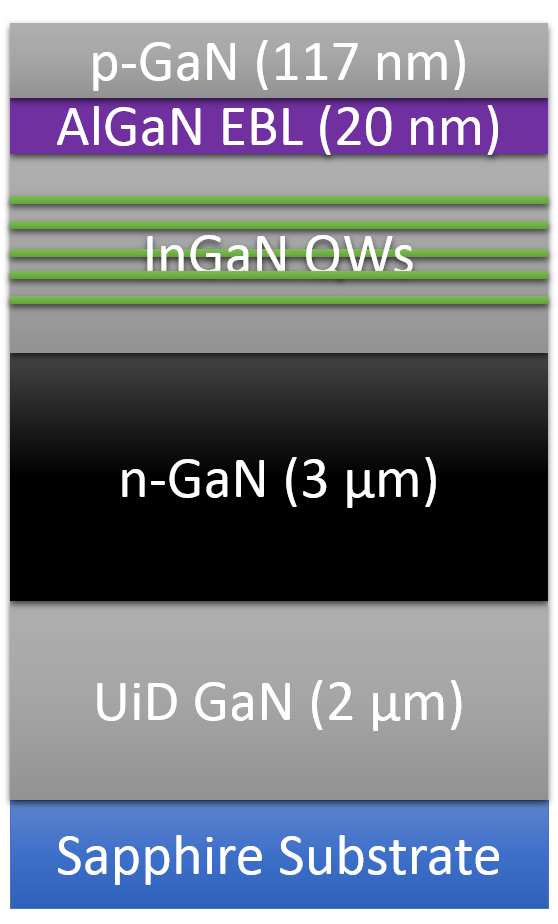
\includegraphics[width=0.4\textwidth]{Figs/Ch3/LEDstruct}
	\caption[h] {LED structure schematic.}
	\label{LEDstruct}
\end{figure}

\FloatBarrier 
The wafers were processed into $1 \times 1 mm^{2}$ side contacted LEDs with thin oxidized Ni/Au current spreading {\it p}-layer Ohmic contact. Ti/Al Ohmic contact stripes were deposited on the {\it n}-layer and the Ni/Au current spreading layer in an interdigitated geometry.\\
QW thickness for both samples was determined from X-ray diffraction \nomenclature[z-XRD]{XRD}{X-ray Diffraction} (XRD) using the method described by Vickers {\it et al.} \cite{Vickers2003}. The QWs were grown using the '2T' method, whereby the growth temperature is ramped up immediately following the InGaN growth under ammonia but without metalorganic fluxes. The barrier growth begins towards the end of the temperature ramp, this typically leads to loss of indium during the temperature ramp which can cause gross well-width fluctuations \cite{Laak2013} but a higher barrier growth temperature is preferable\cite{Oliver2013}. '2T' growth is shown schematically in Fig.\ref{2T}.

\begin{figure}[!ht]
	\centering
	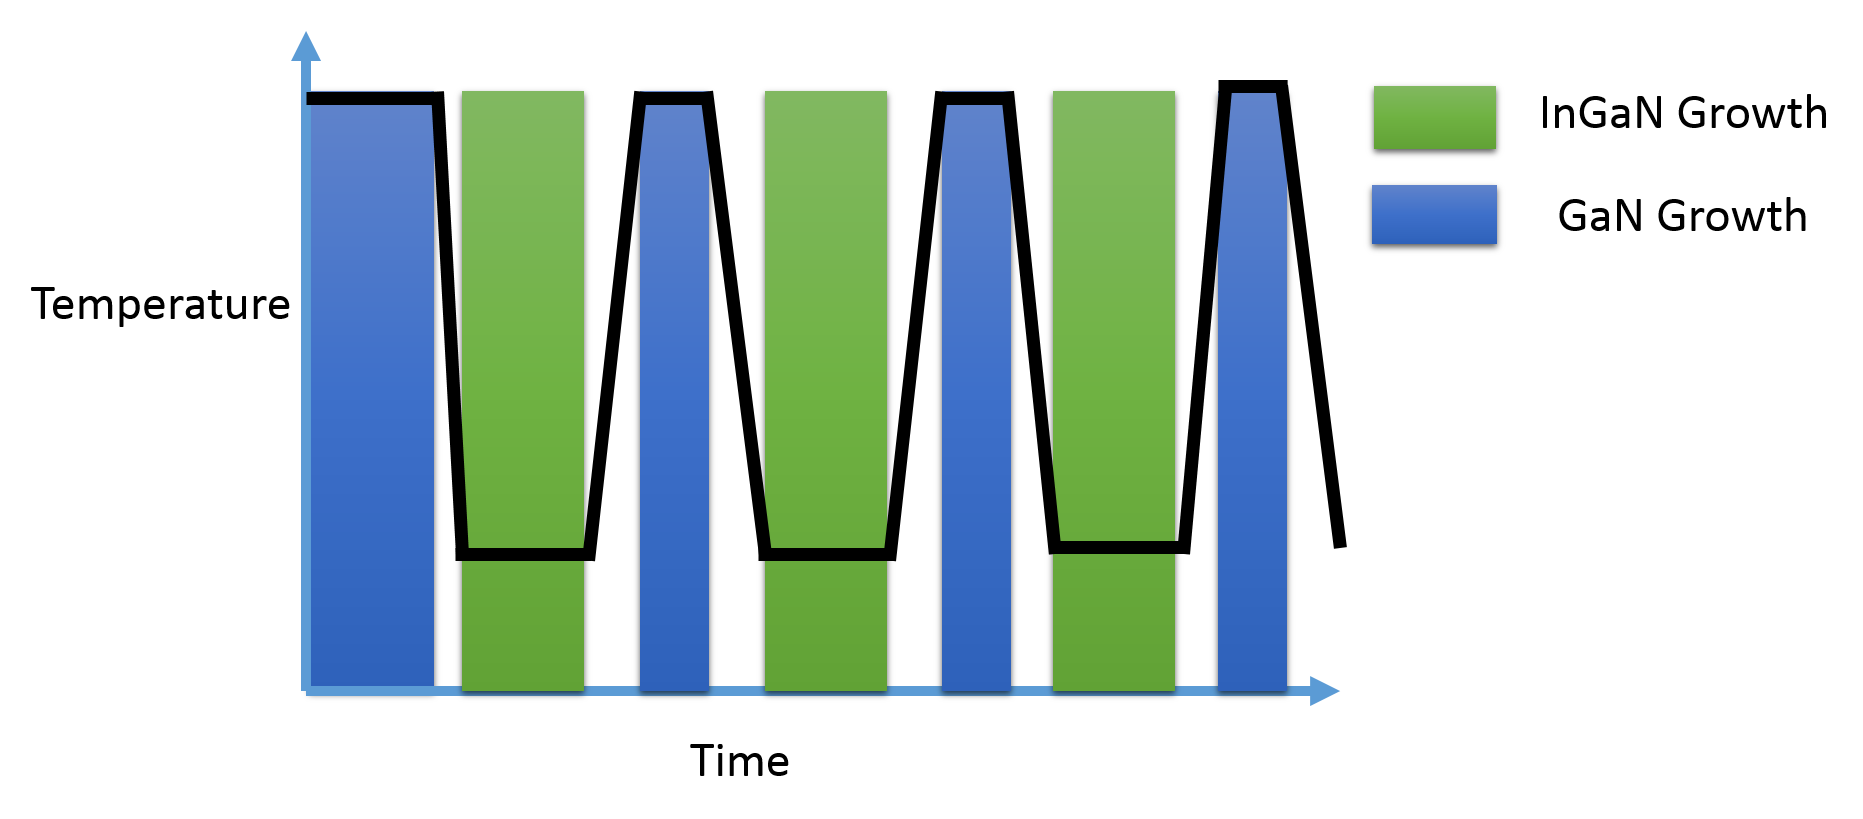
\includegraphics[width=0.9\textwidth]{Figs/Ch3/2T}
	\caption[h] {'2T' growth of InGaN/GaN QWs. GaN QB growth is halted during the temperature ramp. The black trace indicates growth temperature over time.}
	\label{2T}
\end{figure}

\FloatBarrier 

\section{Experimental}

Initial evaluation of the inhomogeneous EL was performed in a Signatone S-1160 probe station under forward bias, as shown in Fig.\ref{probe}.

\begin{figure}[h]
	\begin{subfigure}[t]{0.35\textwidth}
		\centering
		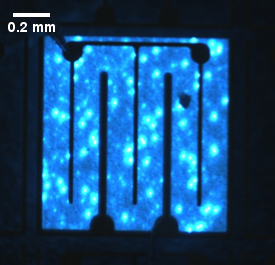
\includegraphics[width = 1\textwidth]{Figs/Ch3/5610.png}
		\caption{}
	\end{subfigure}%
	\hspace*{2cm}
	~	
	\begin{subfigure}[t]{0.35\textwidth}
		\centering
		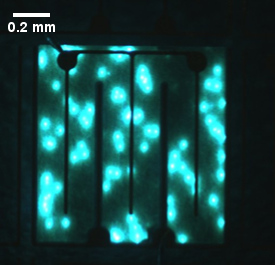
\includegraphics[width=1\textwidth]{Figs/Ch3/5608.png}
		\caption{}
	\end{subfigure}
	\caption {a) C5610A b) C5608A EL under a forward bias of 3V. The bright inhomogeneities are visible in the emission of the LEDs. }
	\label{probe}
\end{figure}
\FloatBarrier


Following this, hyperspectral EL mapping with CL and EBIC were performed using a modified Cameca SX100 electron probe micro-analyser with a custom built cathodoluminescence set-up. Hyperspectral EL measurements were performed under forward bias, enabling the acquisition spatially resolved EL maps of the inhomogeneities. Following the detection of hexagonal defects at the centre of inhomogeneities using SEM-CL, the defects were analyzed using AFM and C-AFM. Finally, FIB/SEM lamella preparation techniques were used to perform HAADF-STEM and STEM-EDX on the defects, allowing for access nanoscale compositional and structural information required to reproduce the EL in simulations.


\subsection{Hyperspectral EL Imaging}
Hyperspectral EL imaging was performed at Strathclyde University with the assistance of Dr Michael Wallace. In order to study the device under forward current, the LED wafers were mounted on TO-5 headers and bonded with 5 µm Al wire. A Keithley Instrument 2401 source meter was used to apply varying forward currents to the devices and thus allow for the collection of EL. \\
Full EL spectra were collected with a spatial resolution of approximately 3 µm and analysed using custom software developed by Dr. Paul Edwards, allowing for 2-D maps of EL peak intensity, position and FWHM. At each pixel in the map, a full EL spectrum was collected by an Andor CCD camera. A full set of data extracted from the hyperspectral EL mapping is shown in Fig.\ref{ELfull}

\begin{figure}[!ht]
	\centering
	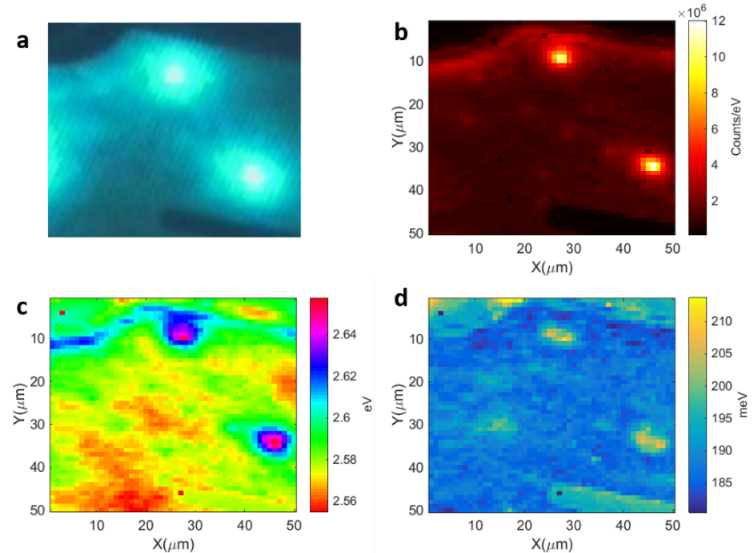
\includegraphics[width=0.8\textwidth]{Figs/Ch3/ELfull}
	\caption[h] {a) Probe station image b) EL peak intensity, c) EL peak energy and d) EL FWHM extracted by fitting the hyperspectral EL data under a forward current of 10 mA}
	\label{ELfull}
\end{figure}

\FloatBarrier 

It is interesting to note that from this representative data set, the inhomogeneities observed are brighter by a factor of $\sim 6$, blue-shifted in terms of peak energy by $\sim 0.08$ eV and have a larger FWHM. Although these values were observed to shift based on injection current, the overall trend observed in all data sets for both LED devices is represented by Fig.\ref{ELfull}.

\subsubsection{Current Dependent EL Measurements}

Current dependent hyperspectral EL maps of the same area were performed, in order to examine the behaviour of the inhomogeneities with increasing current relative to the 'uniform' background. The peak intensities and peak energies for injection currents for device C5610A ranging from 1-500 mA are shown in Figures \ref{peak5610} and \ref{centre5610} respectively. 

\begin{figure}
	\begin{subfigure}[b]{0.48\textwidth}
		\centering
		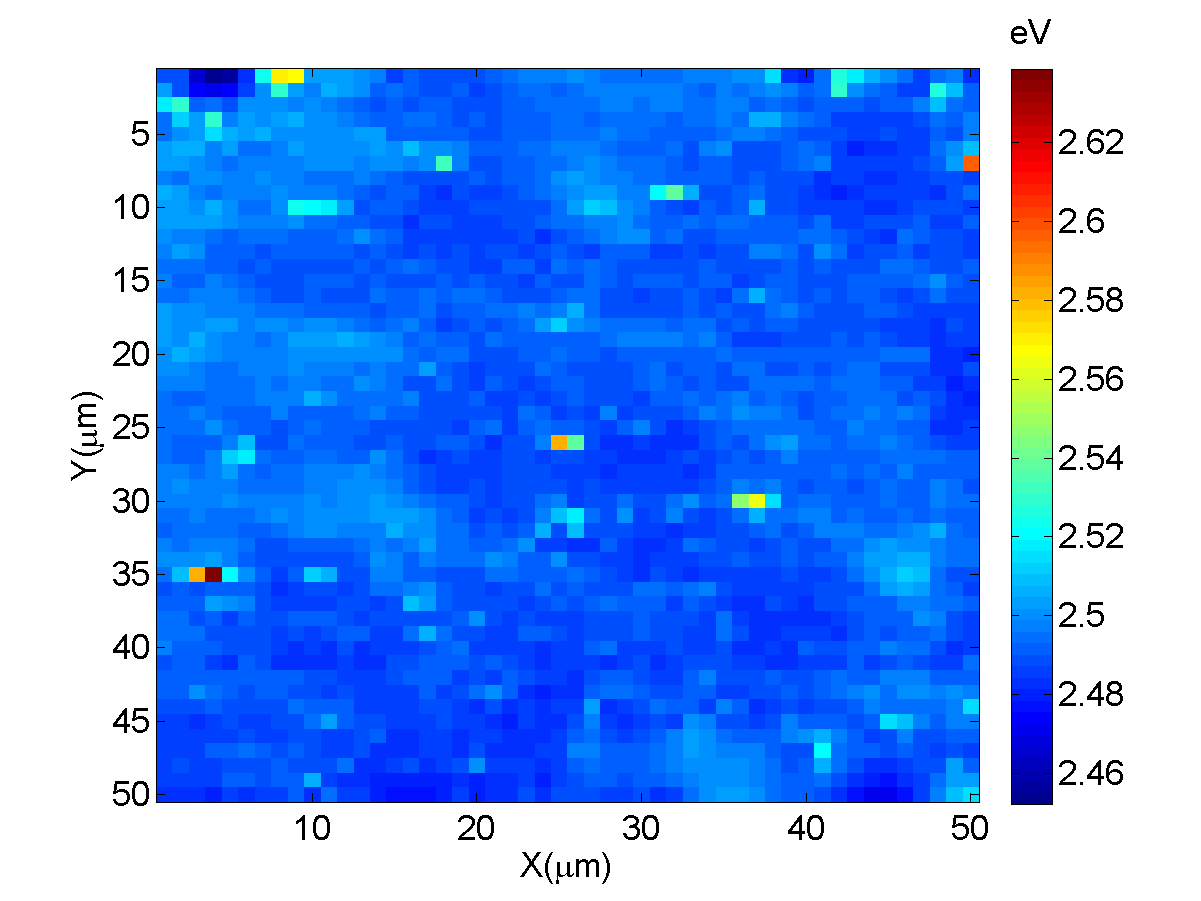
\includegraphics[width=1\linewidth]{Figs/Ch3/1}
		\caption{1 mA}
	\end{subfigure}%
	\hspace*\fill
	\begin{subfigure}[b]{0.48\textwidth}
		\centering
		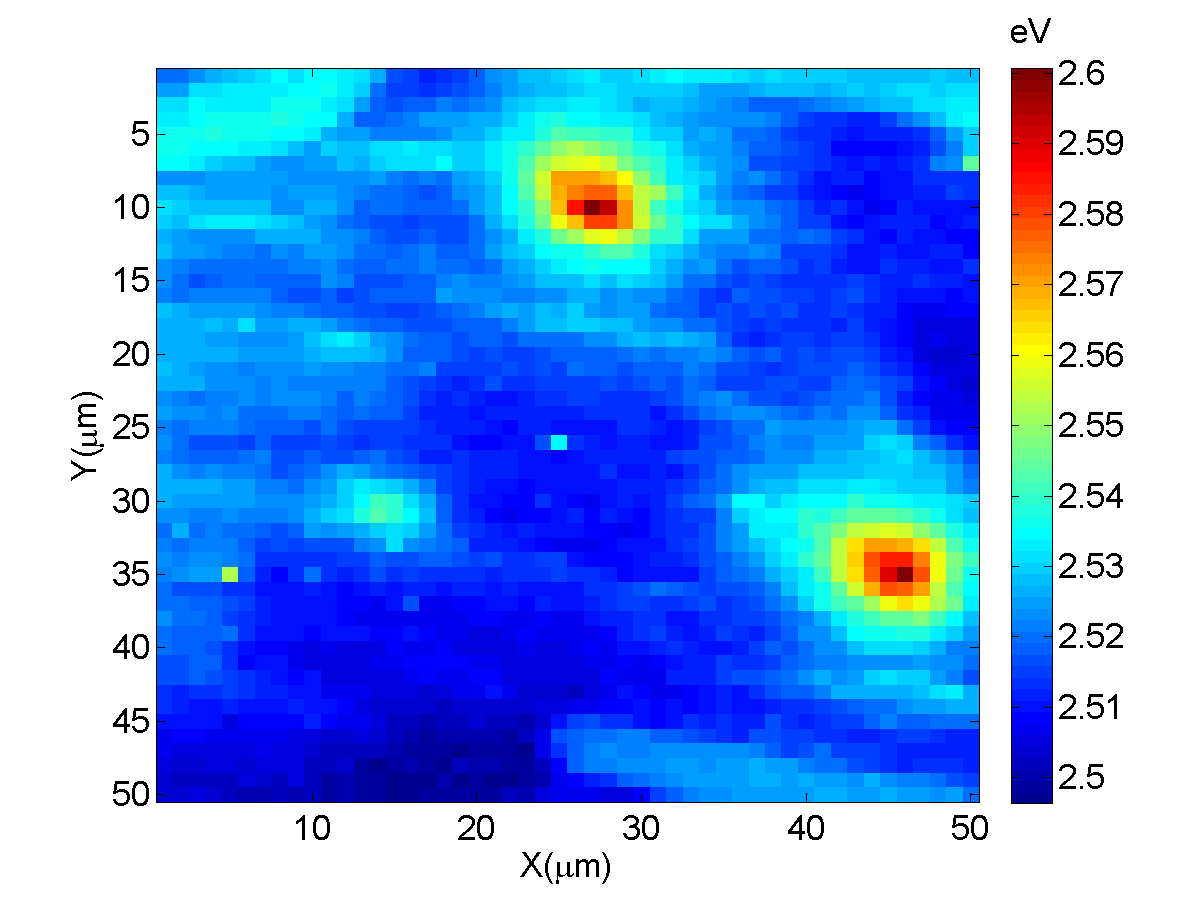
\includegraphics[width=1\linewidth]{Figs/Ch3/5}
		\caption{5 mA}		
	\end{subfigure}%
	
	\medskip
	\begin{subfigure}[b]{0.48\textwidth}
		\centering
		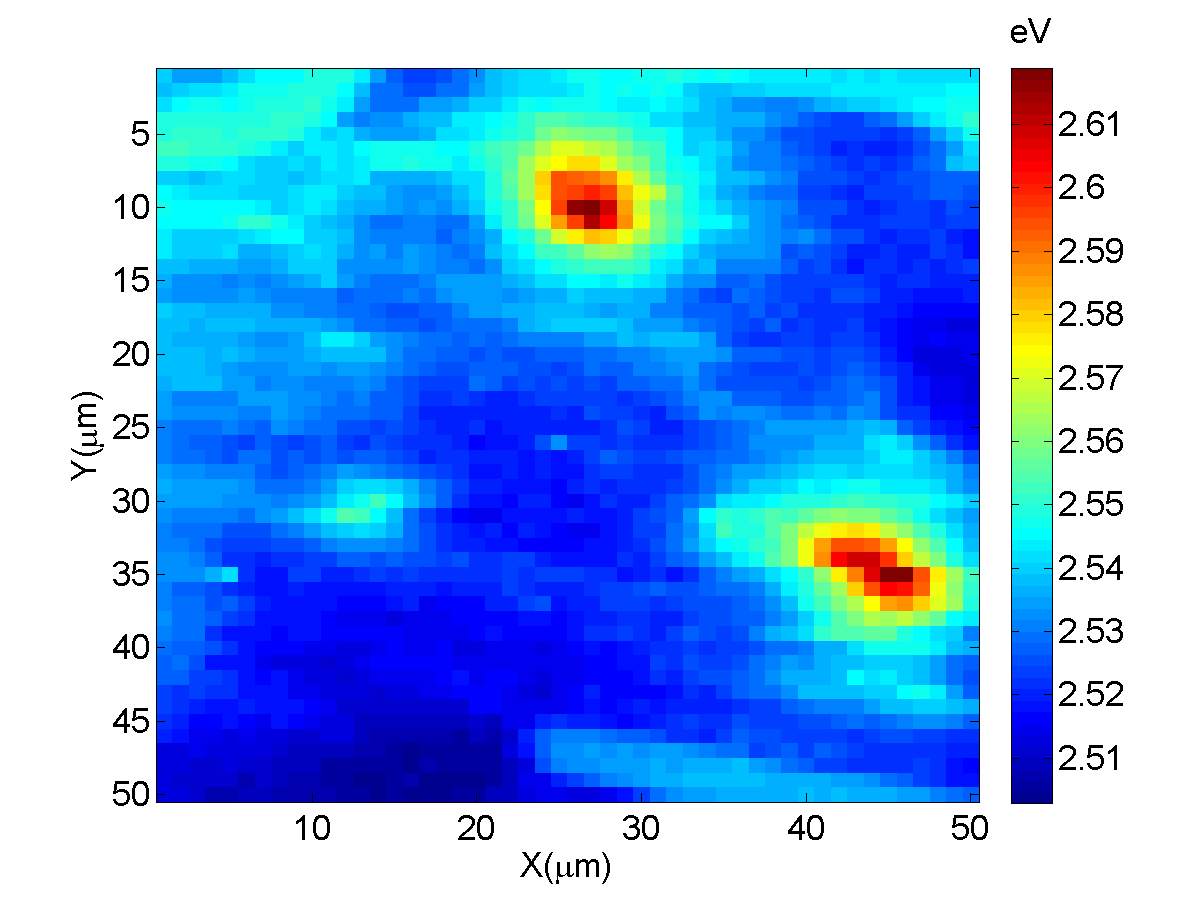
\includegraphics[width=1\linewidth]{Figs/Ch3/10}
		\caption{10 mA}
	\end{subfigure}%
	\hspace*\fill
	\begin{subfigure}[b]{0.48\textwidth}
		\centering
		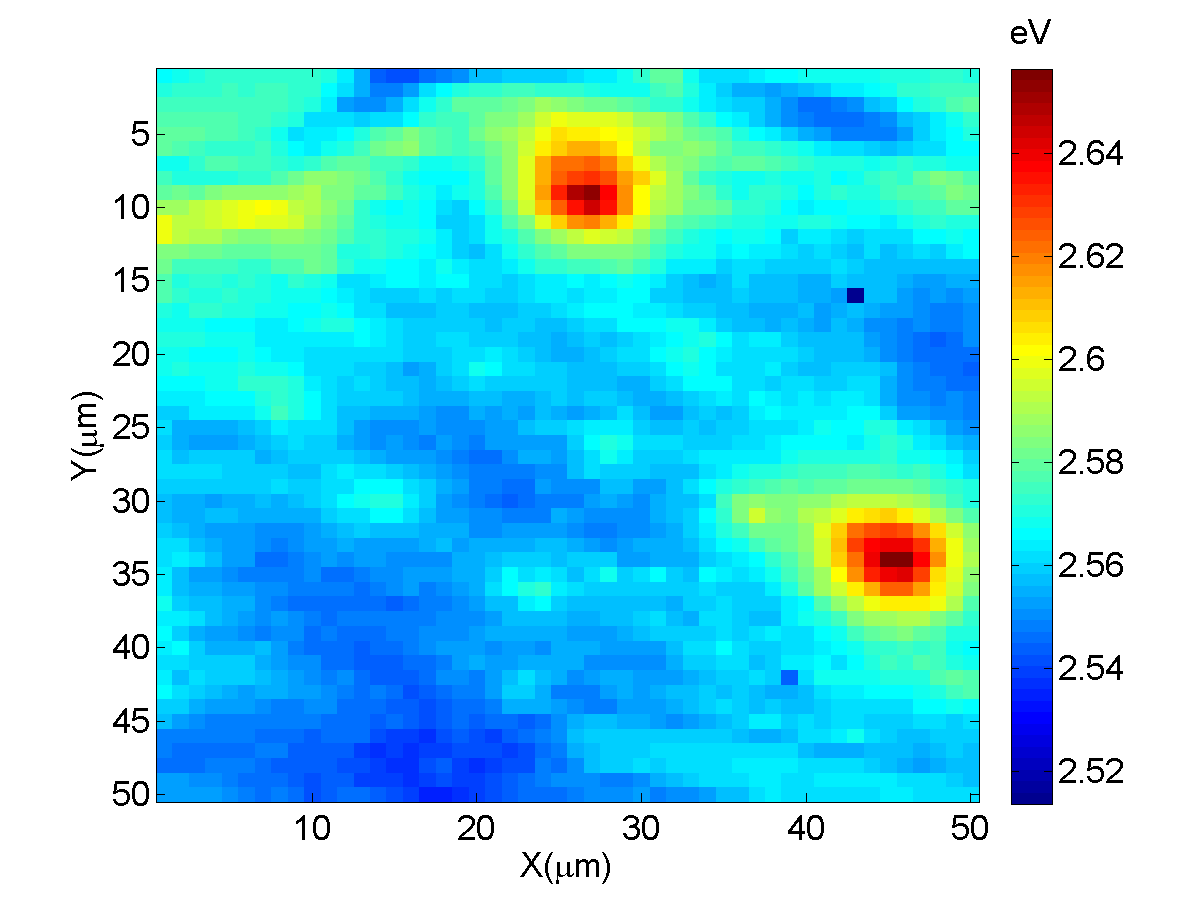
\includegraphics[width=1\linewidth]{Figs/Ch3/50}
		\caption{50 mA}		
	\end{subfigure}%
	
	\medskip
	\begin{subfigure}[b]{0.48\textwidth}
		\centering
		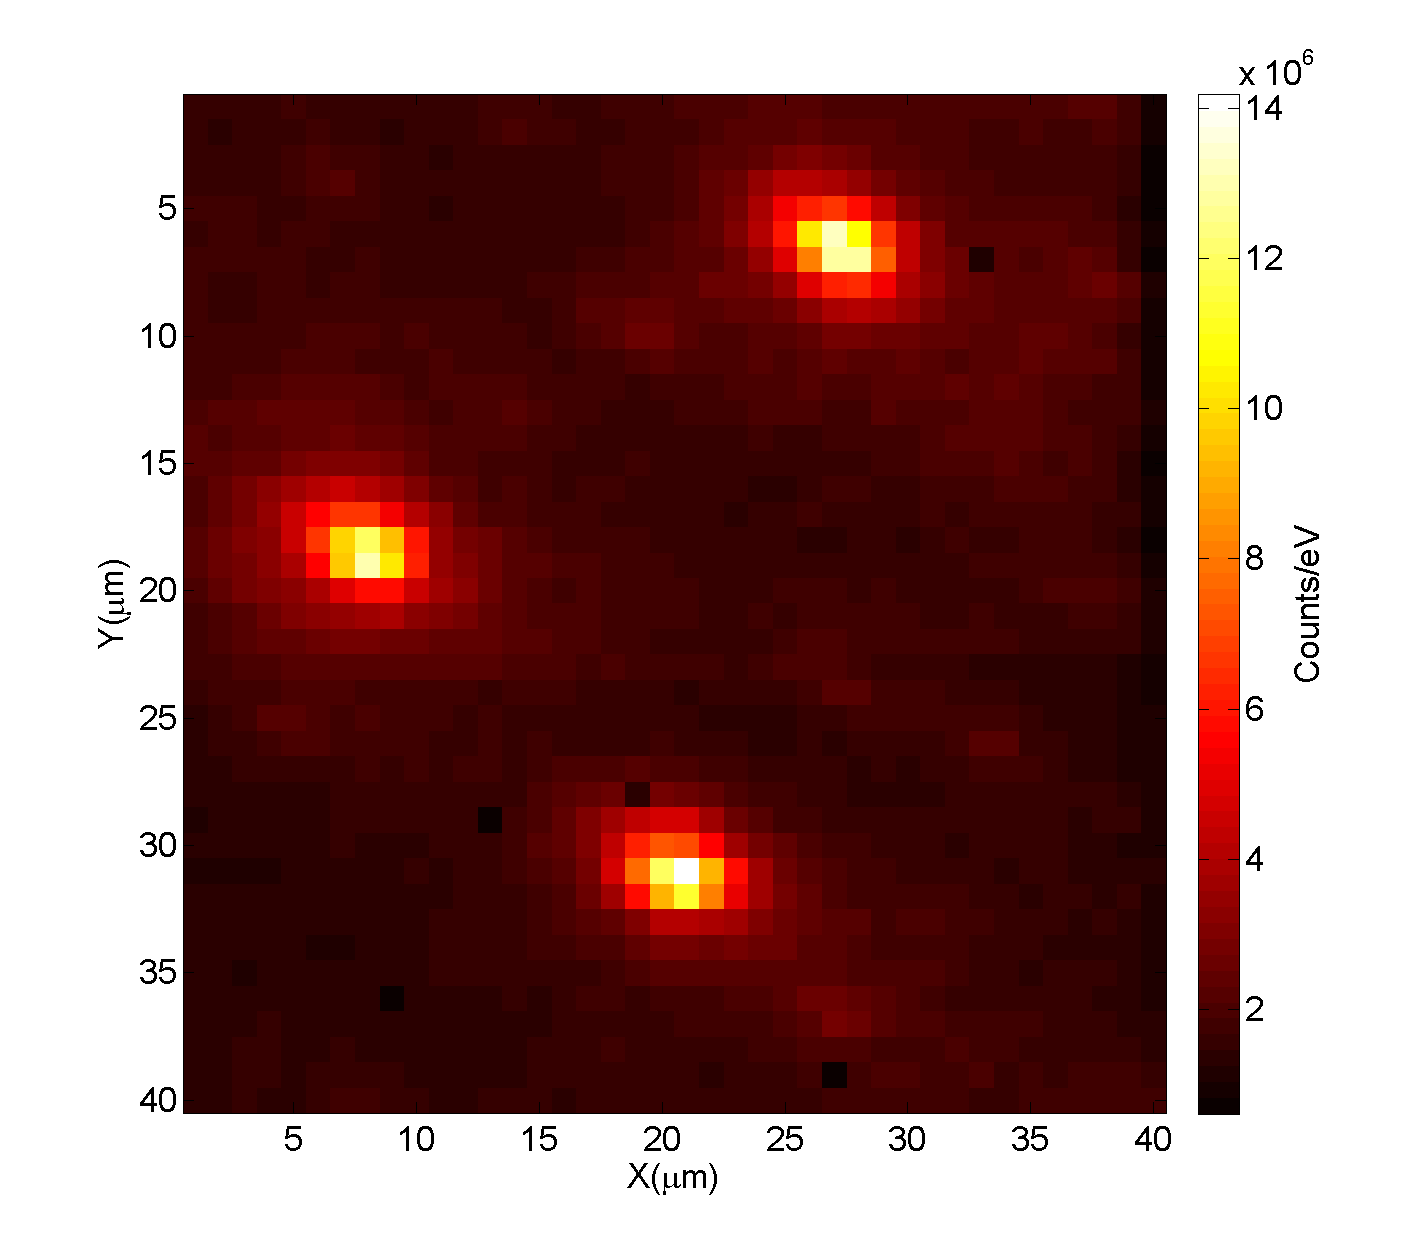
\includegraphics[width=1\linewidth]{Figs/Ch3/100}
		\caption{100 mA}
	\end{subfigure}%
	\hspace*\fill
	\begin{subfigure}[b]{0.48\textwidth}
		\centering
		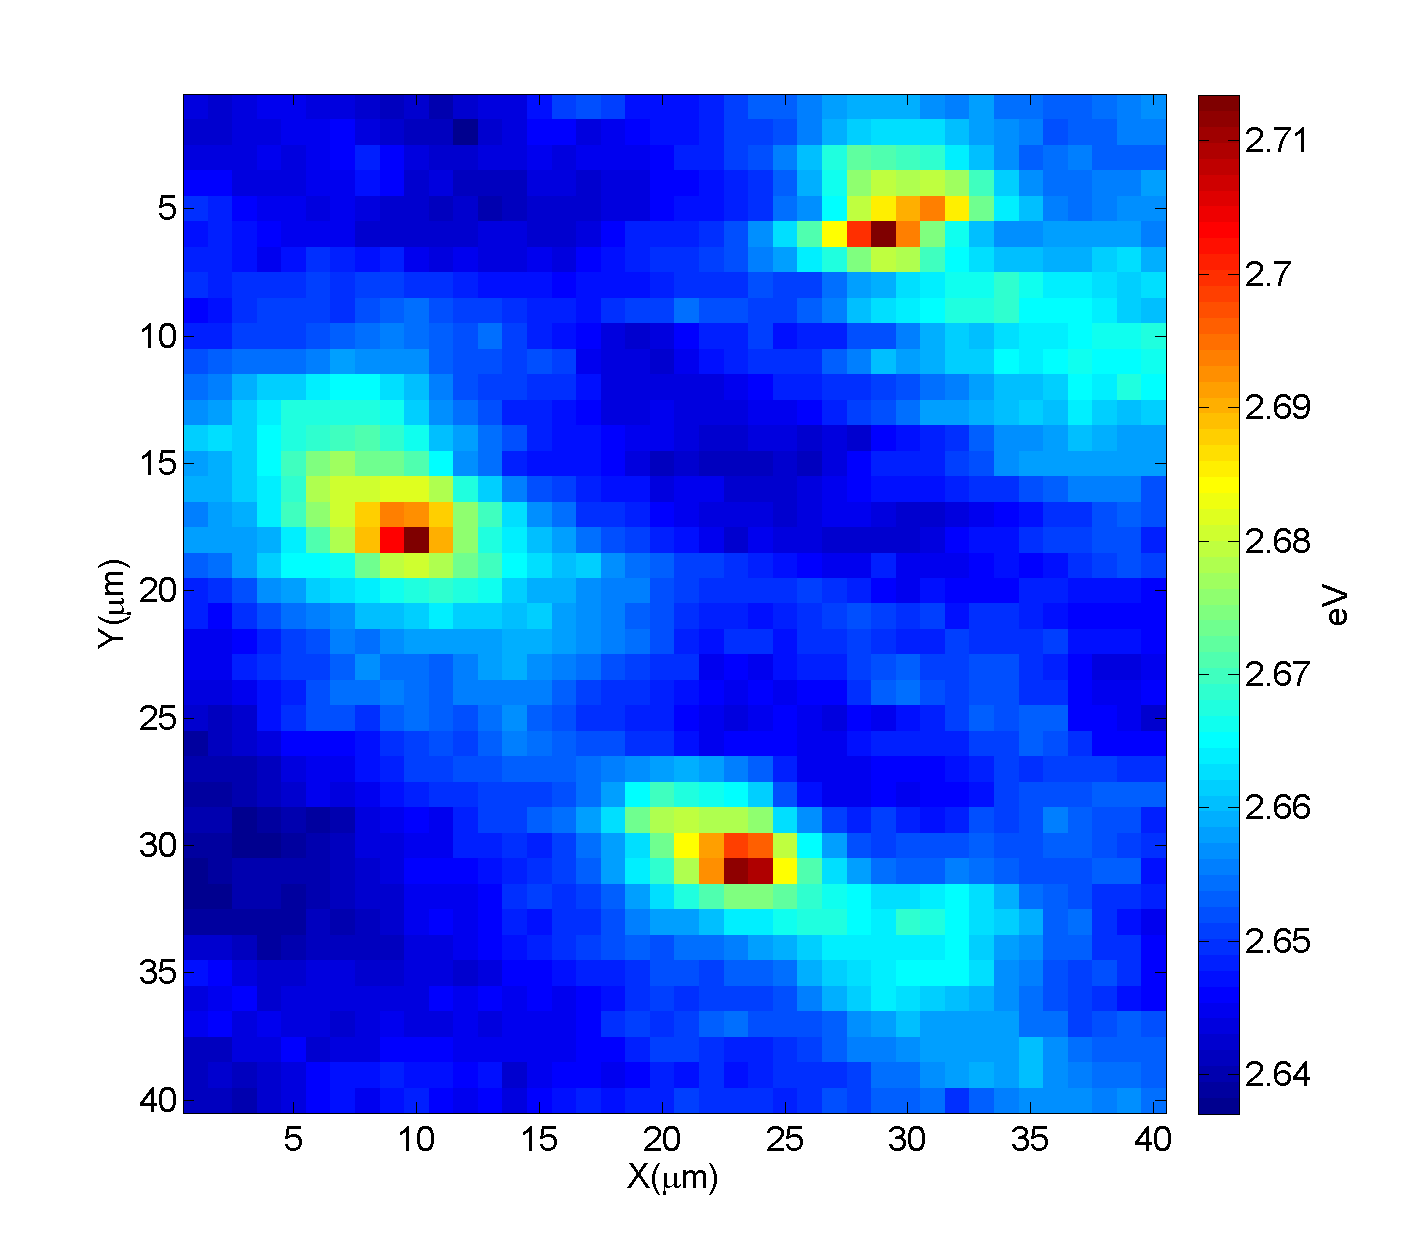
\includegraphics[width=1\linewidth]{Figs/Ch3/500}
		\caption{500 mA}		
	\end{subfigure}%
	
	\caption{Peak intensity for varying injection current for C5610.}
	\label{peak5610}
\end{figure}

\begin{figure}
	\begin{subfigure}[b]{0.48\textwidth}
		\centering
		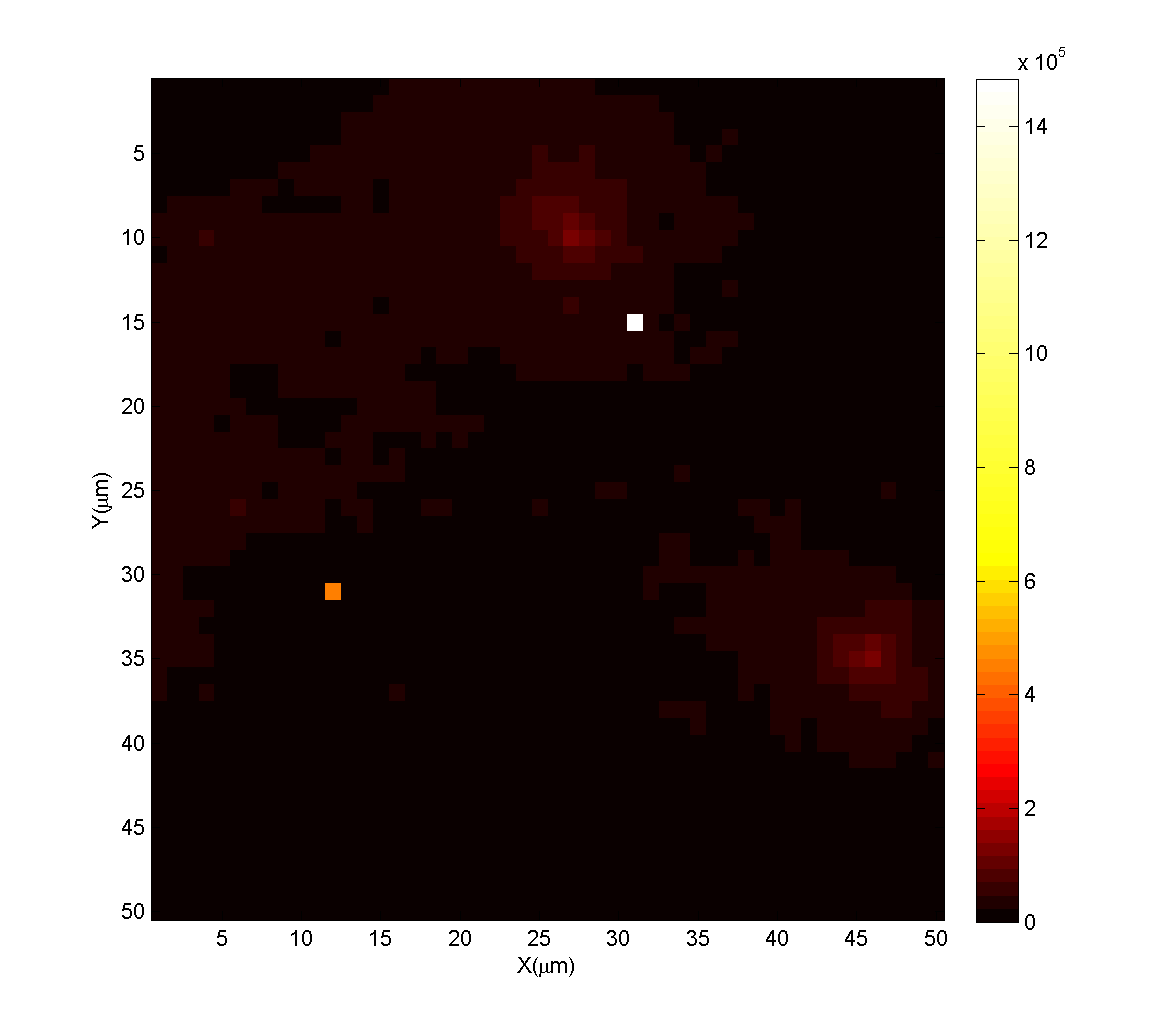
\includegraphics[width=1\linewidth]{Figs/Ch3/1c}
		\caption{1 mA}
	\end{subfigure}%
	\hspace*\fill
	\begin{subfigure}[b]{0.48\textwidth}
		\centering
		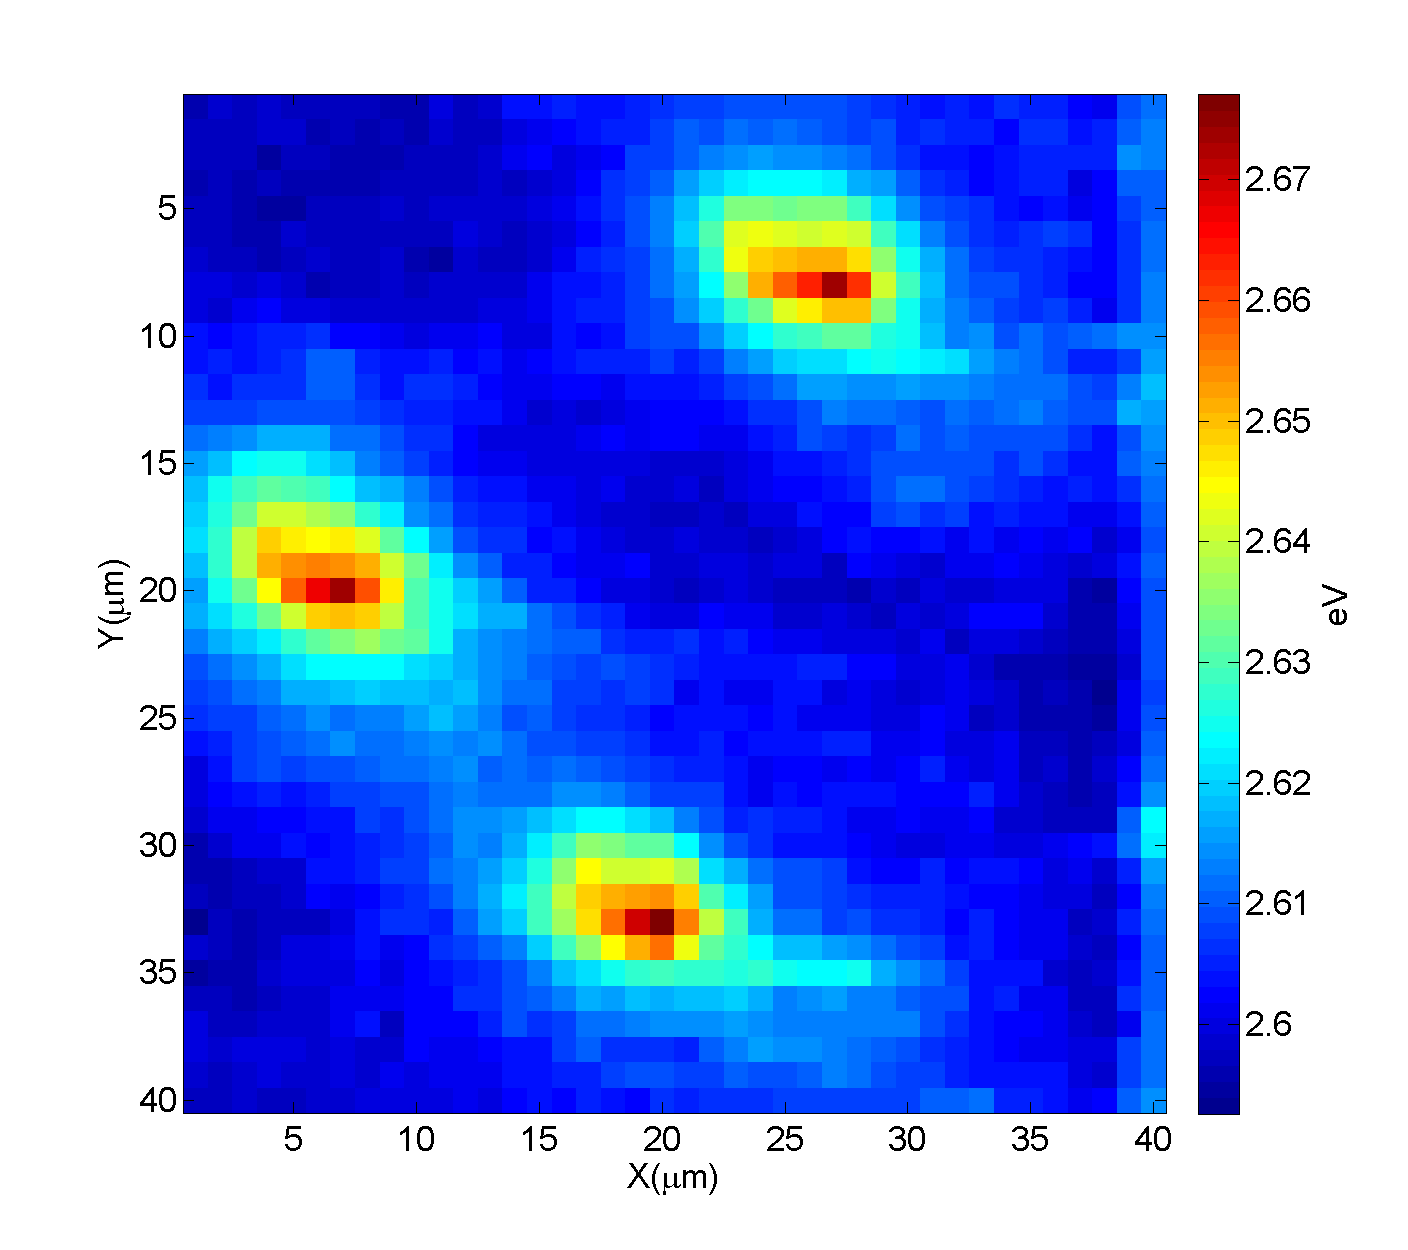
\includegraphics[width=1\linewidth]{Figs/Ch3/5c}
		\caption{5 mA}		
	\end{subfigure}%
	
	\medskip
	\begin{subfigure}[b]{0.48\textwidth}
		\centering
		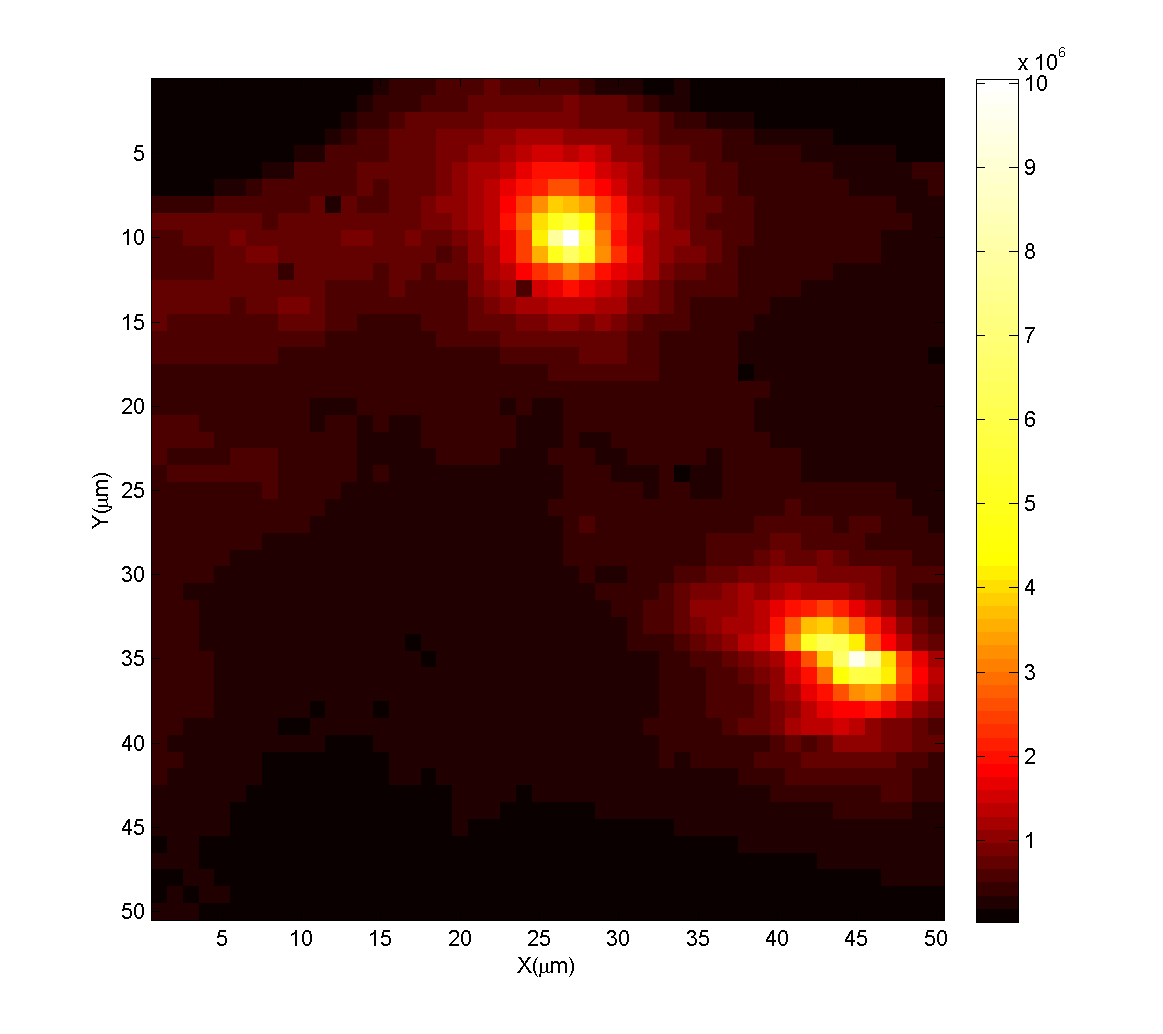
\includegraphics[width=1\linewidth]{Figs/Ch3/10c}
		\caption{10 mA}
	\end{subfigure}%
	\hspace*\fill
	\begin{subfigure}[b]{0.48\textwidth}
		\centering
		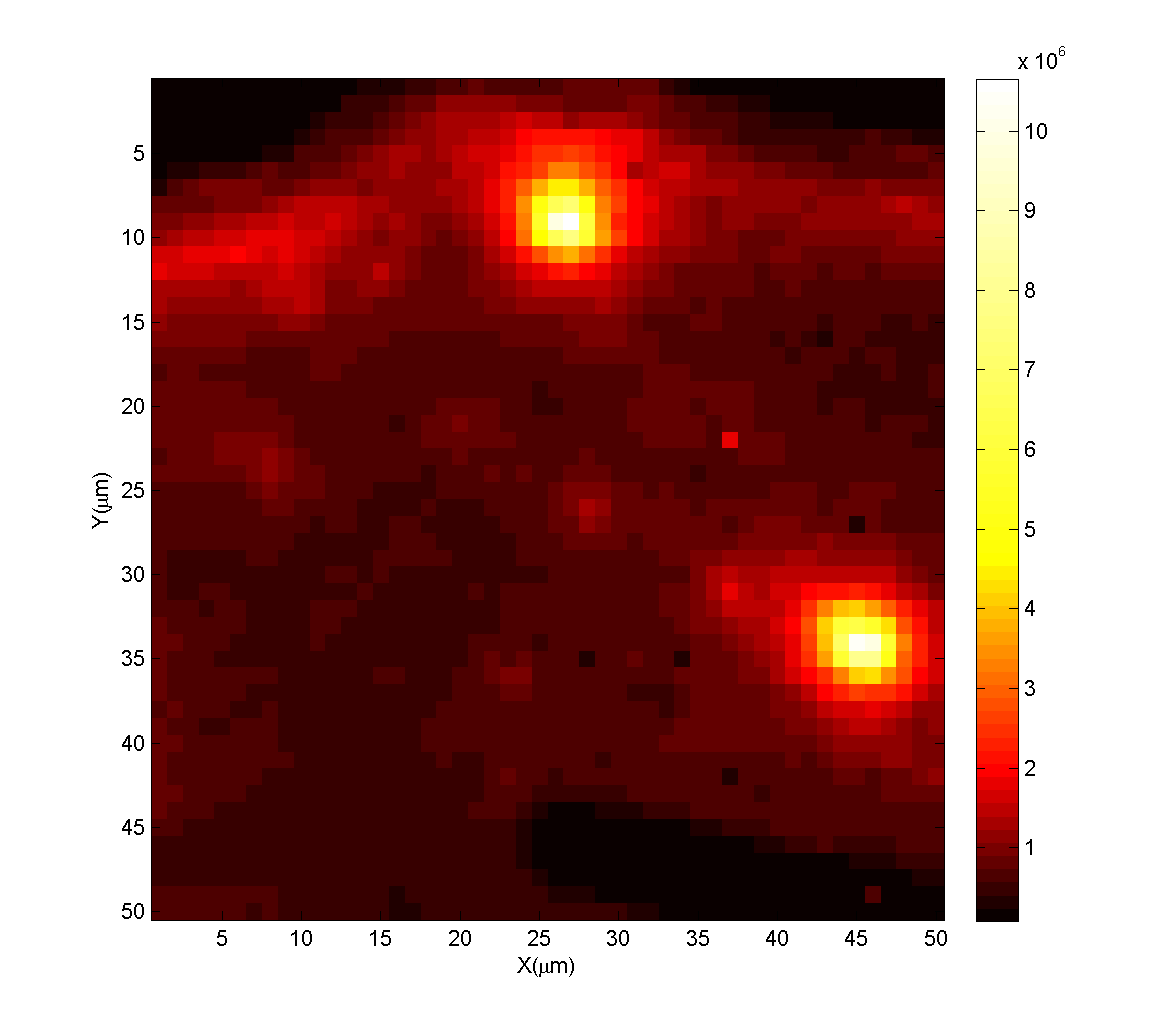
\includegraphics[width=1\linewidth]{Figs/Ch3/50c}
		\caption{50 mA}		
	\end{subfigure}%
	
	\medskip
	\begin{subfigure}[b]{0.48\textwidth}
		\centering
		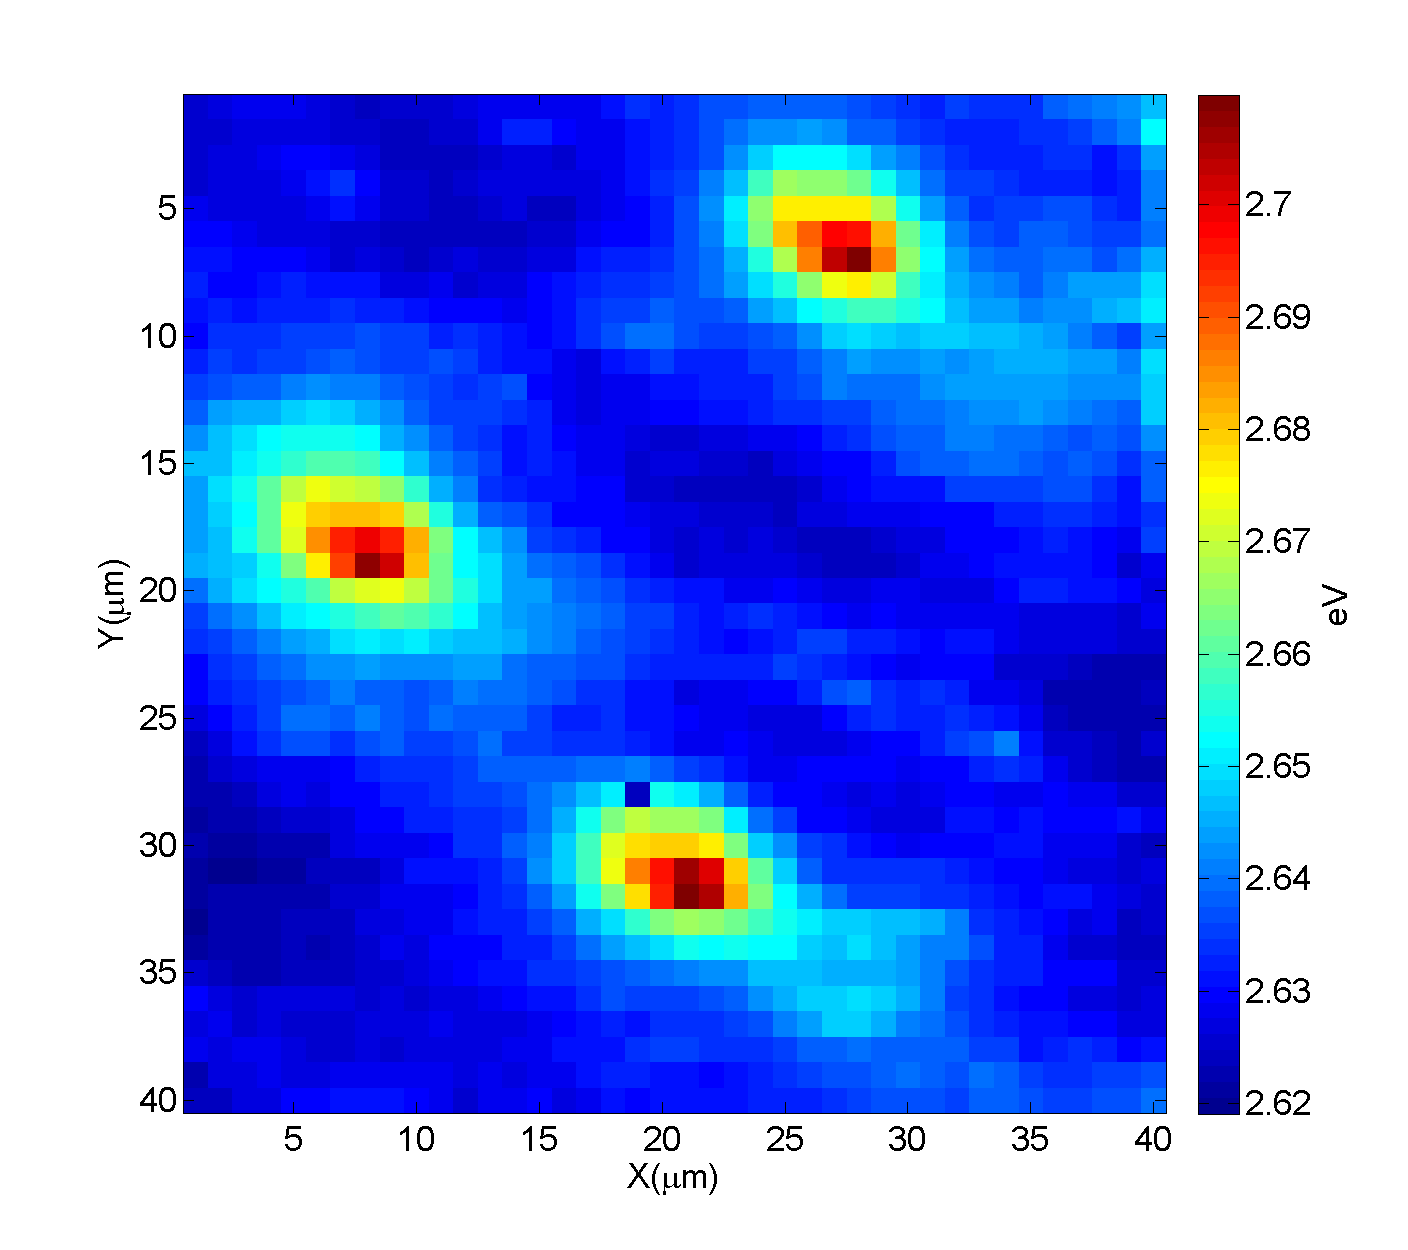
\includegraphics[width=1\linewidth]{Figs/Ch3/100c}
		\caption{100 mA}
	\end{subfigure}%
	\hspace*\fill
	\begin{subfigure}[b]{0.48\textwidth}
		\centering
		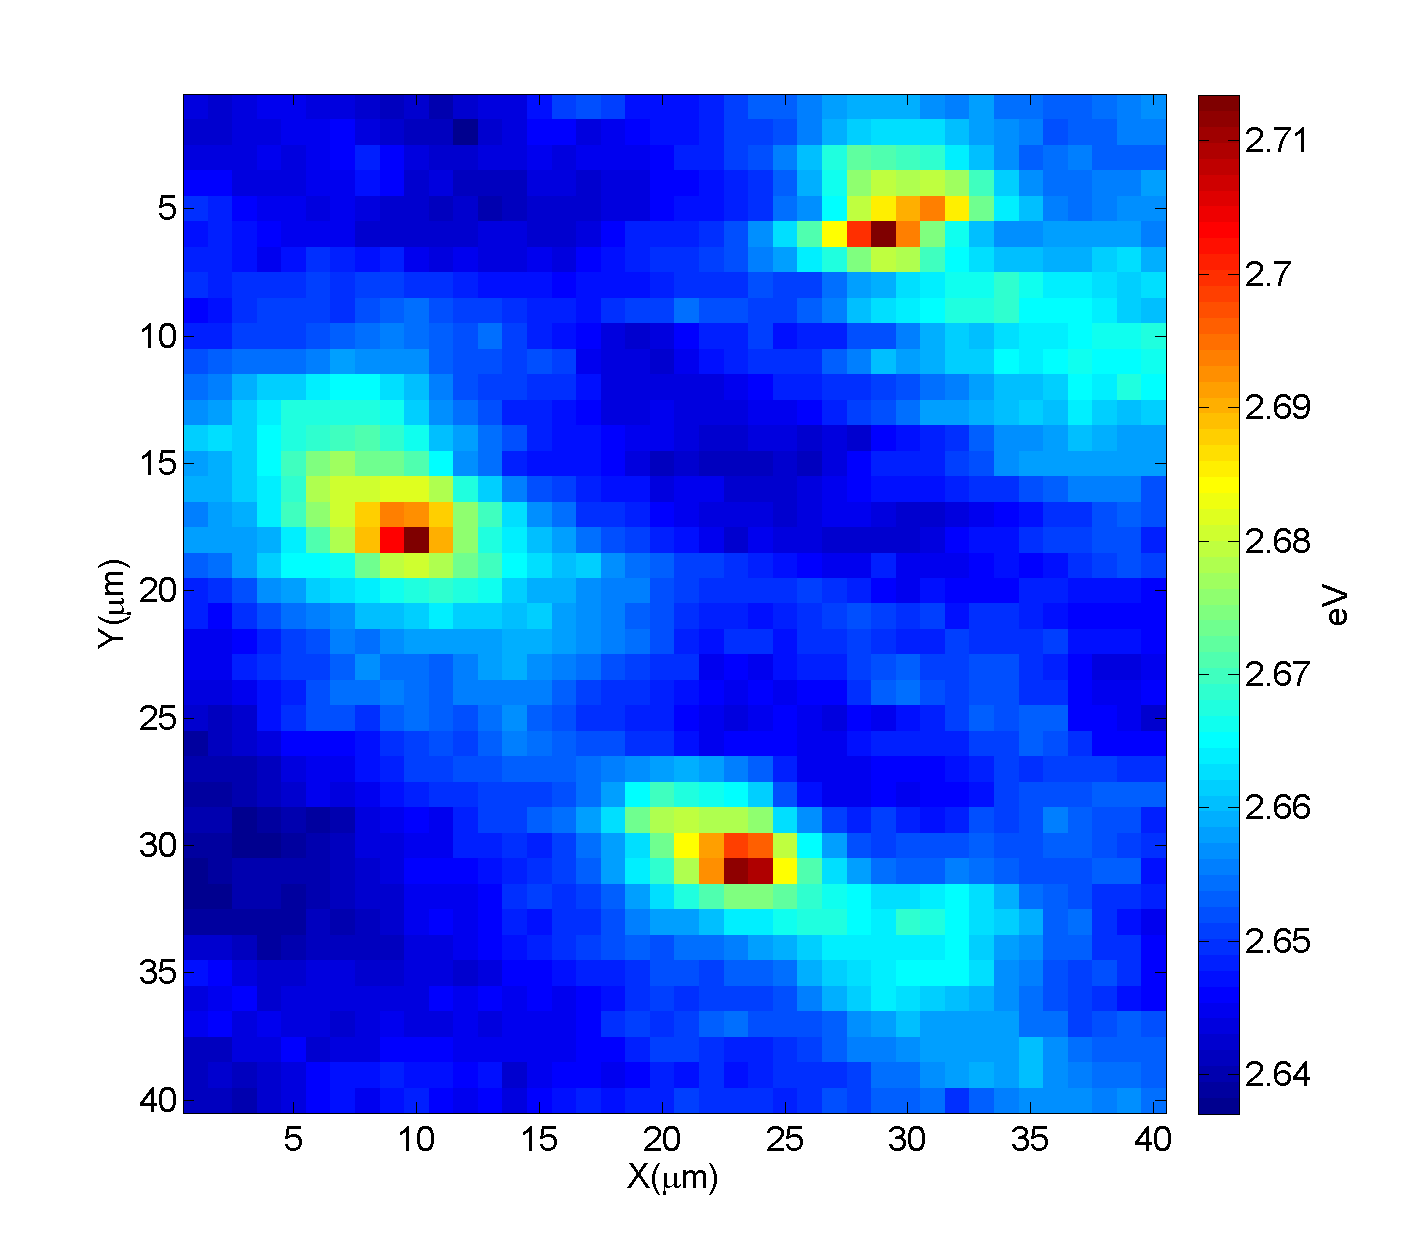
\includegraphics[width=1\linewidth]{Figs/Ch3/500c}
		\caption{500 mA}		
	\end{subfigure}%
	
	\caption{Peak energy for varying injection current for C5610.}
	\label{centre5610}
\end{figure}

\FloatBarrier

The spatially resolved EL data shown in Figures \ref{peak5610} and \ref{centre5610} allow for the comparison between areas containing the inhomogeneities and the 'background' EL by thresholding the data set. This is demonstrated in Fig. \ref{5610peakcomp} which shows the behaviour of both the inhomogeneities (lablled 'spots') and the averaged background peak intensity with increasing injection current.
\begin{figure}[!ht]
	\centering
	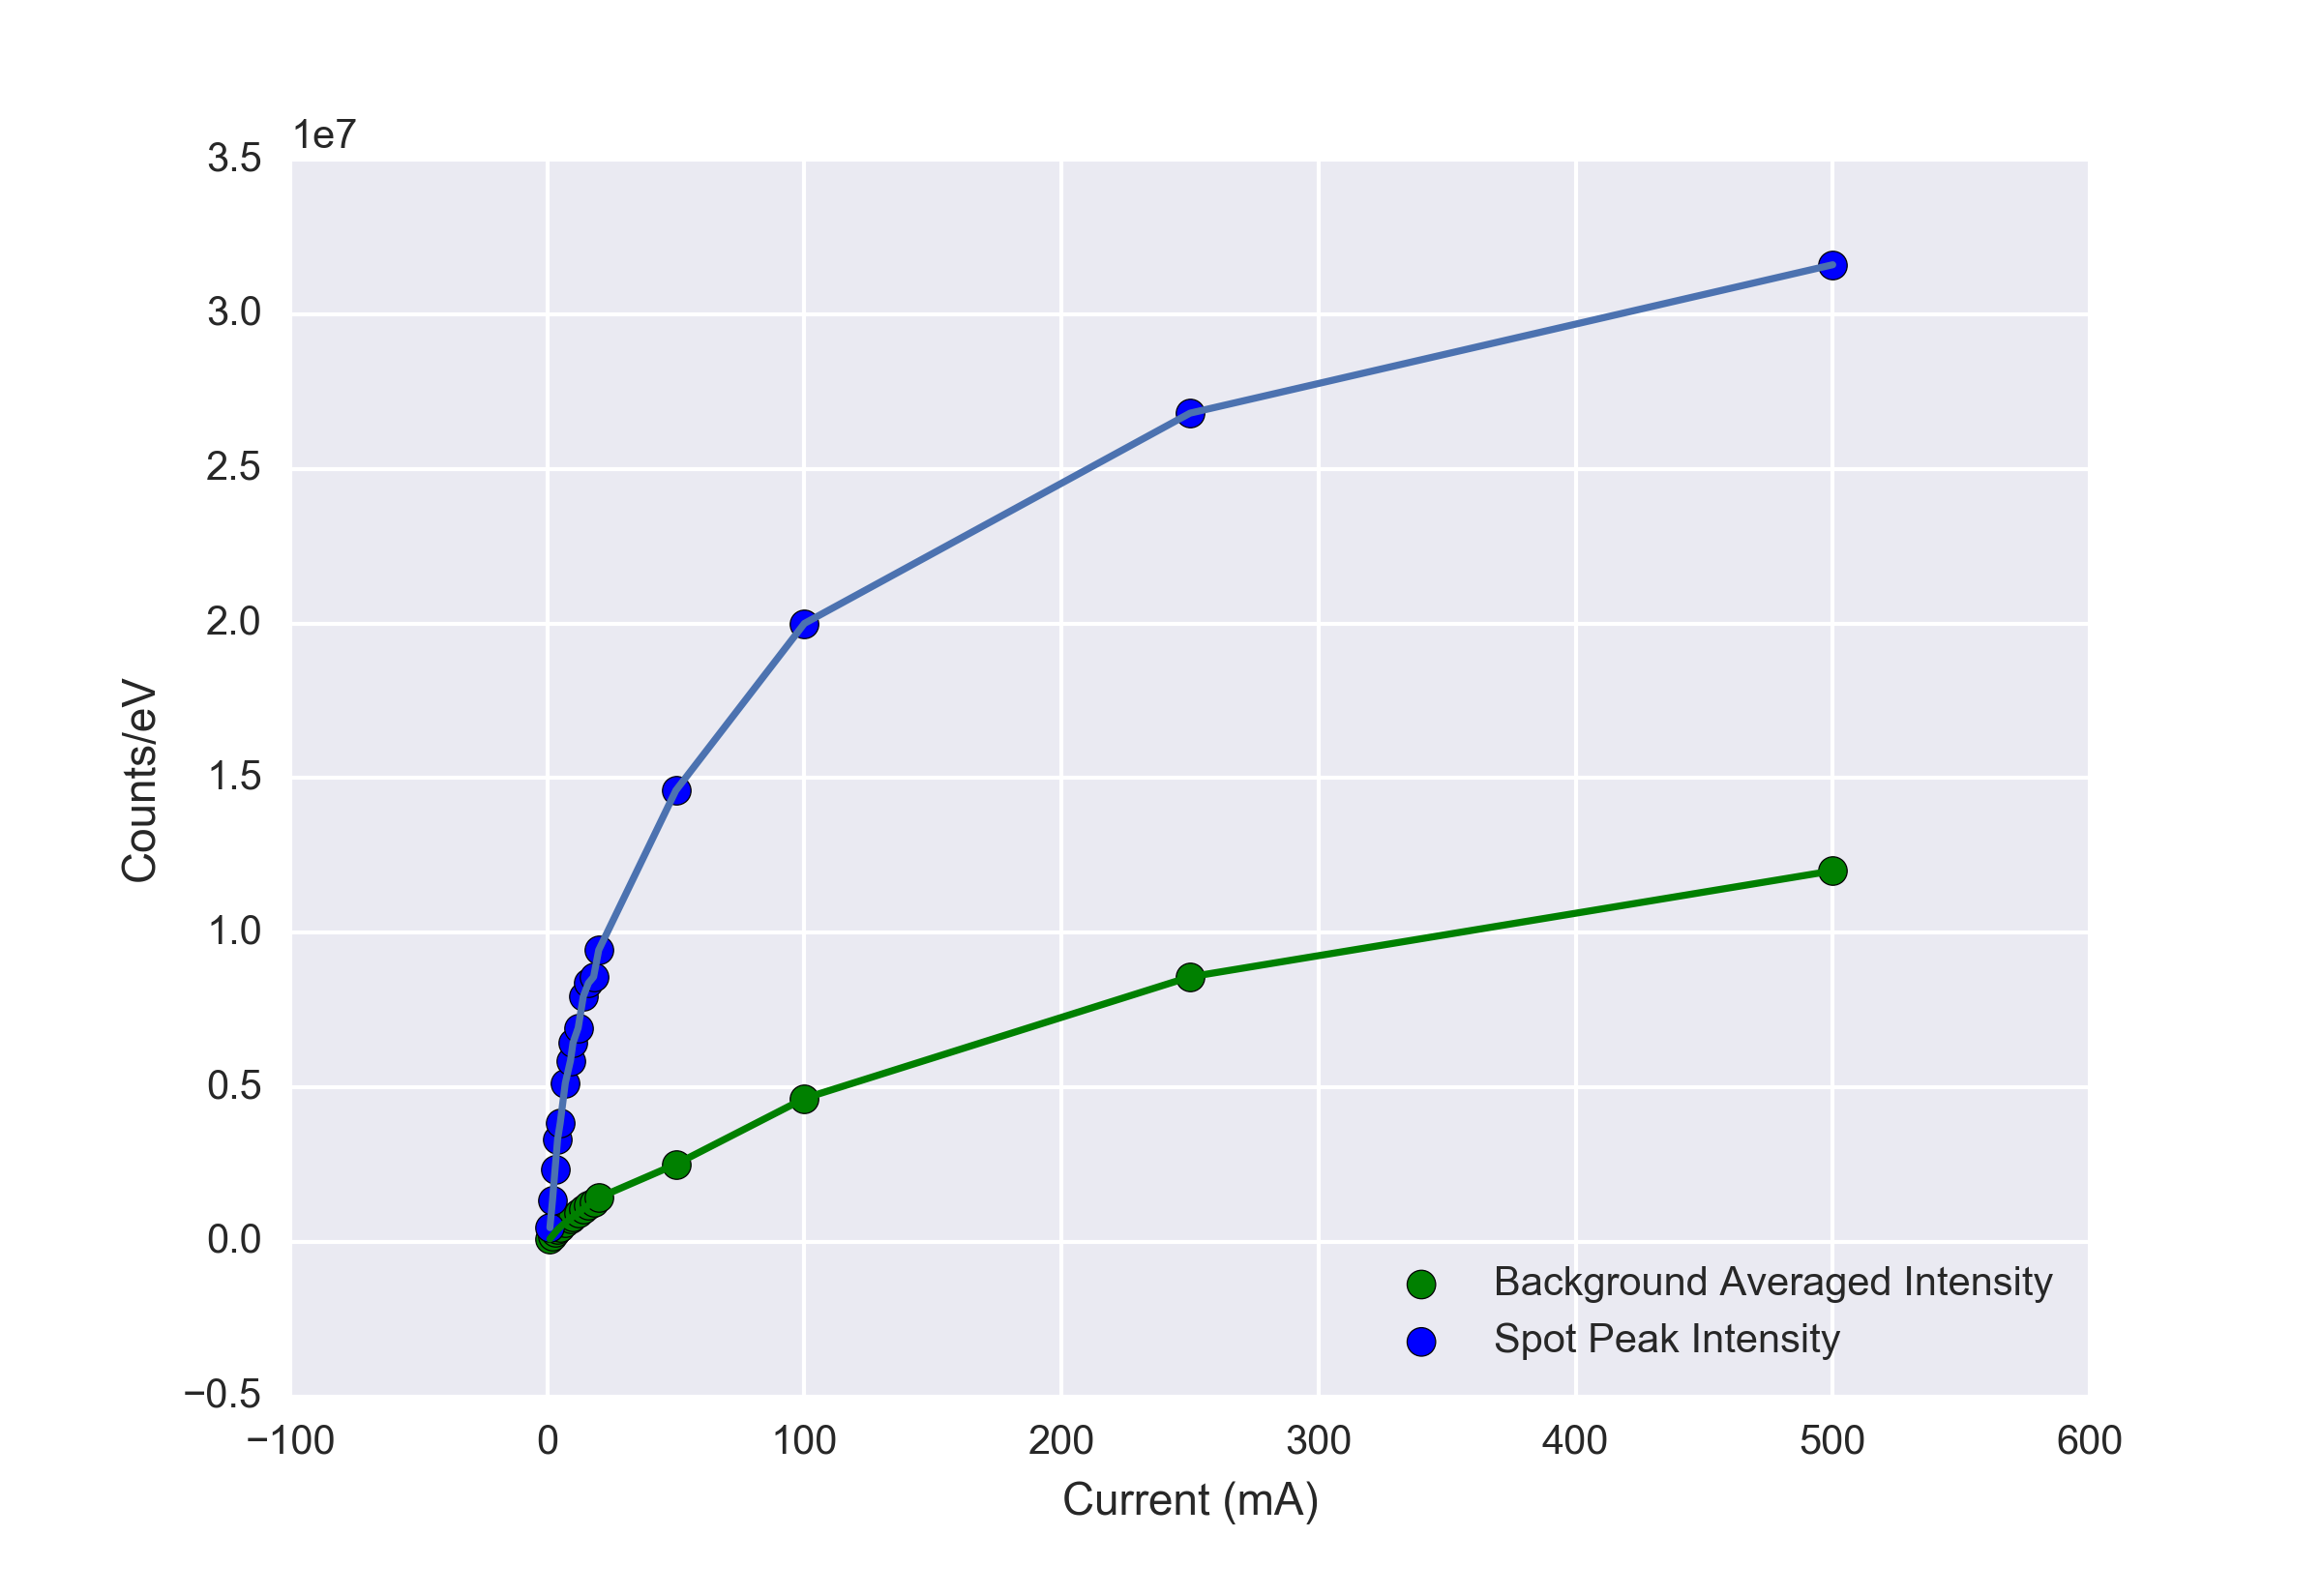
\includegraphics[width=0.8\textwidth]{Figs/Ch3/Peakcomp5610.png}
	\caption[h] {Spot and background average peak intensity against injection current}
	\label{5610peakcomp}
\end{figure}

\FloatBarrier 
It is interesting to note that Fig.\ref{5610peakcomp} shows the inhomogeneities experience a far sharper initial increase in peak intensity relative to the background based on the hyperspectral EL data fitting in the current range 0-50 mA, perhaps indicating enhanced current injection in the areas exhibiting the inhomogeneities.\\
Fig. \ref{5610centrecomp} shows the same current dependent comparison for background and inhomogeneity peak energy. Here we see the same trend, in that the inhomogeneity exhibits a larger current-induced blueshift in the 0-50 mA range relative to the background. The origin of the current-dependent blueshift in InGaN QW structures is attributed to the screening of the QCSE by the additional carriers injected into the wells \cite{Ryou2009}, and as such indicates the inhomogeneities are regions experiencing higher current injection relative to the background.

\begin{figure}[!ht]
	\centering
	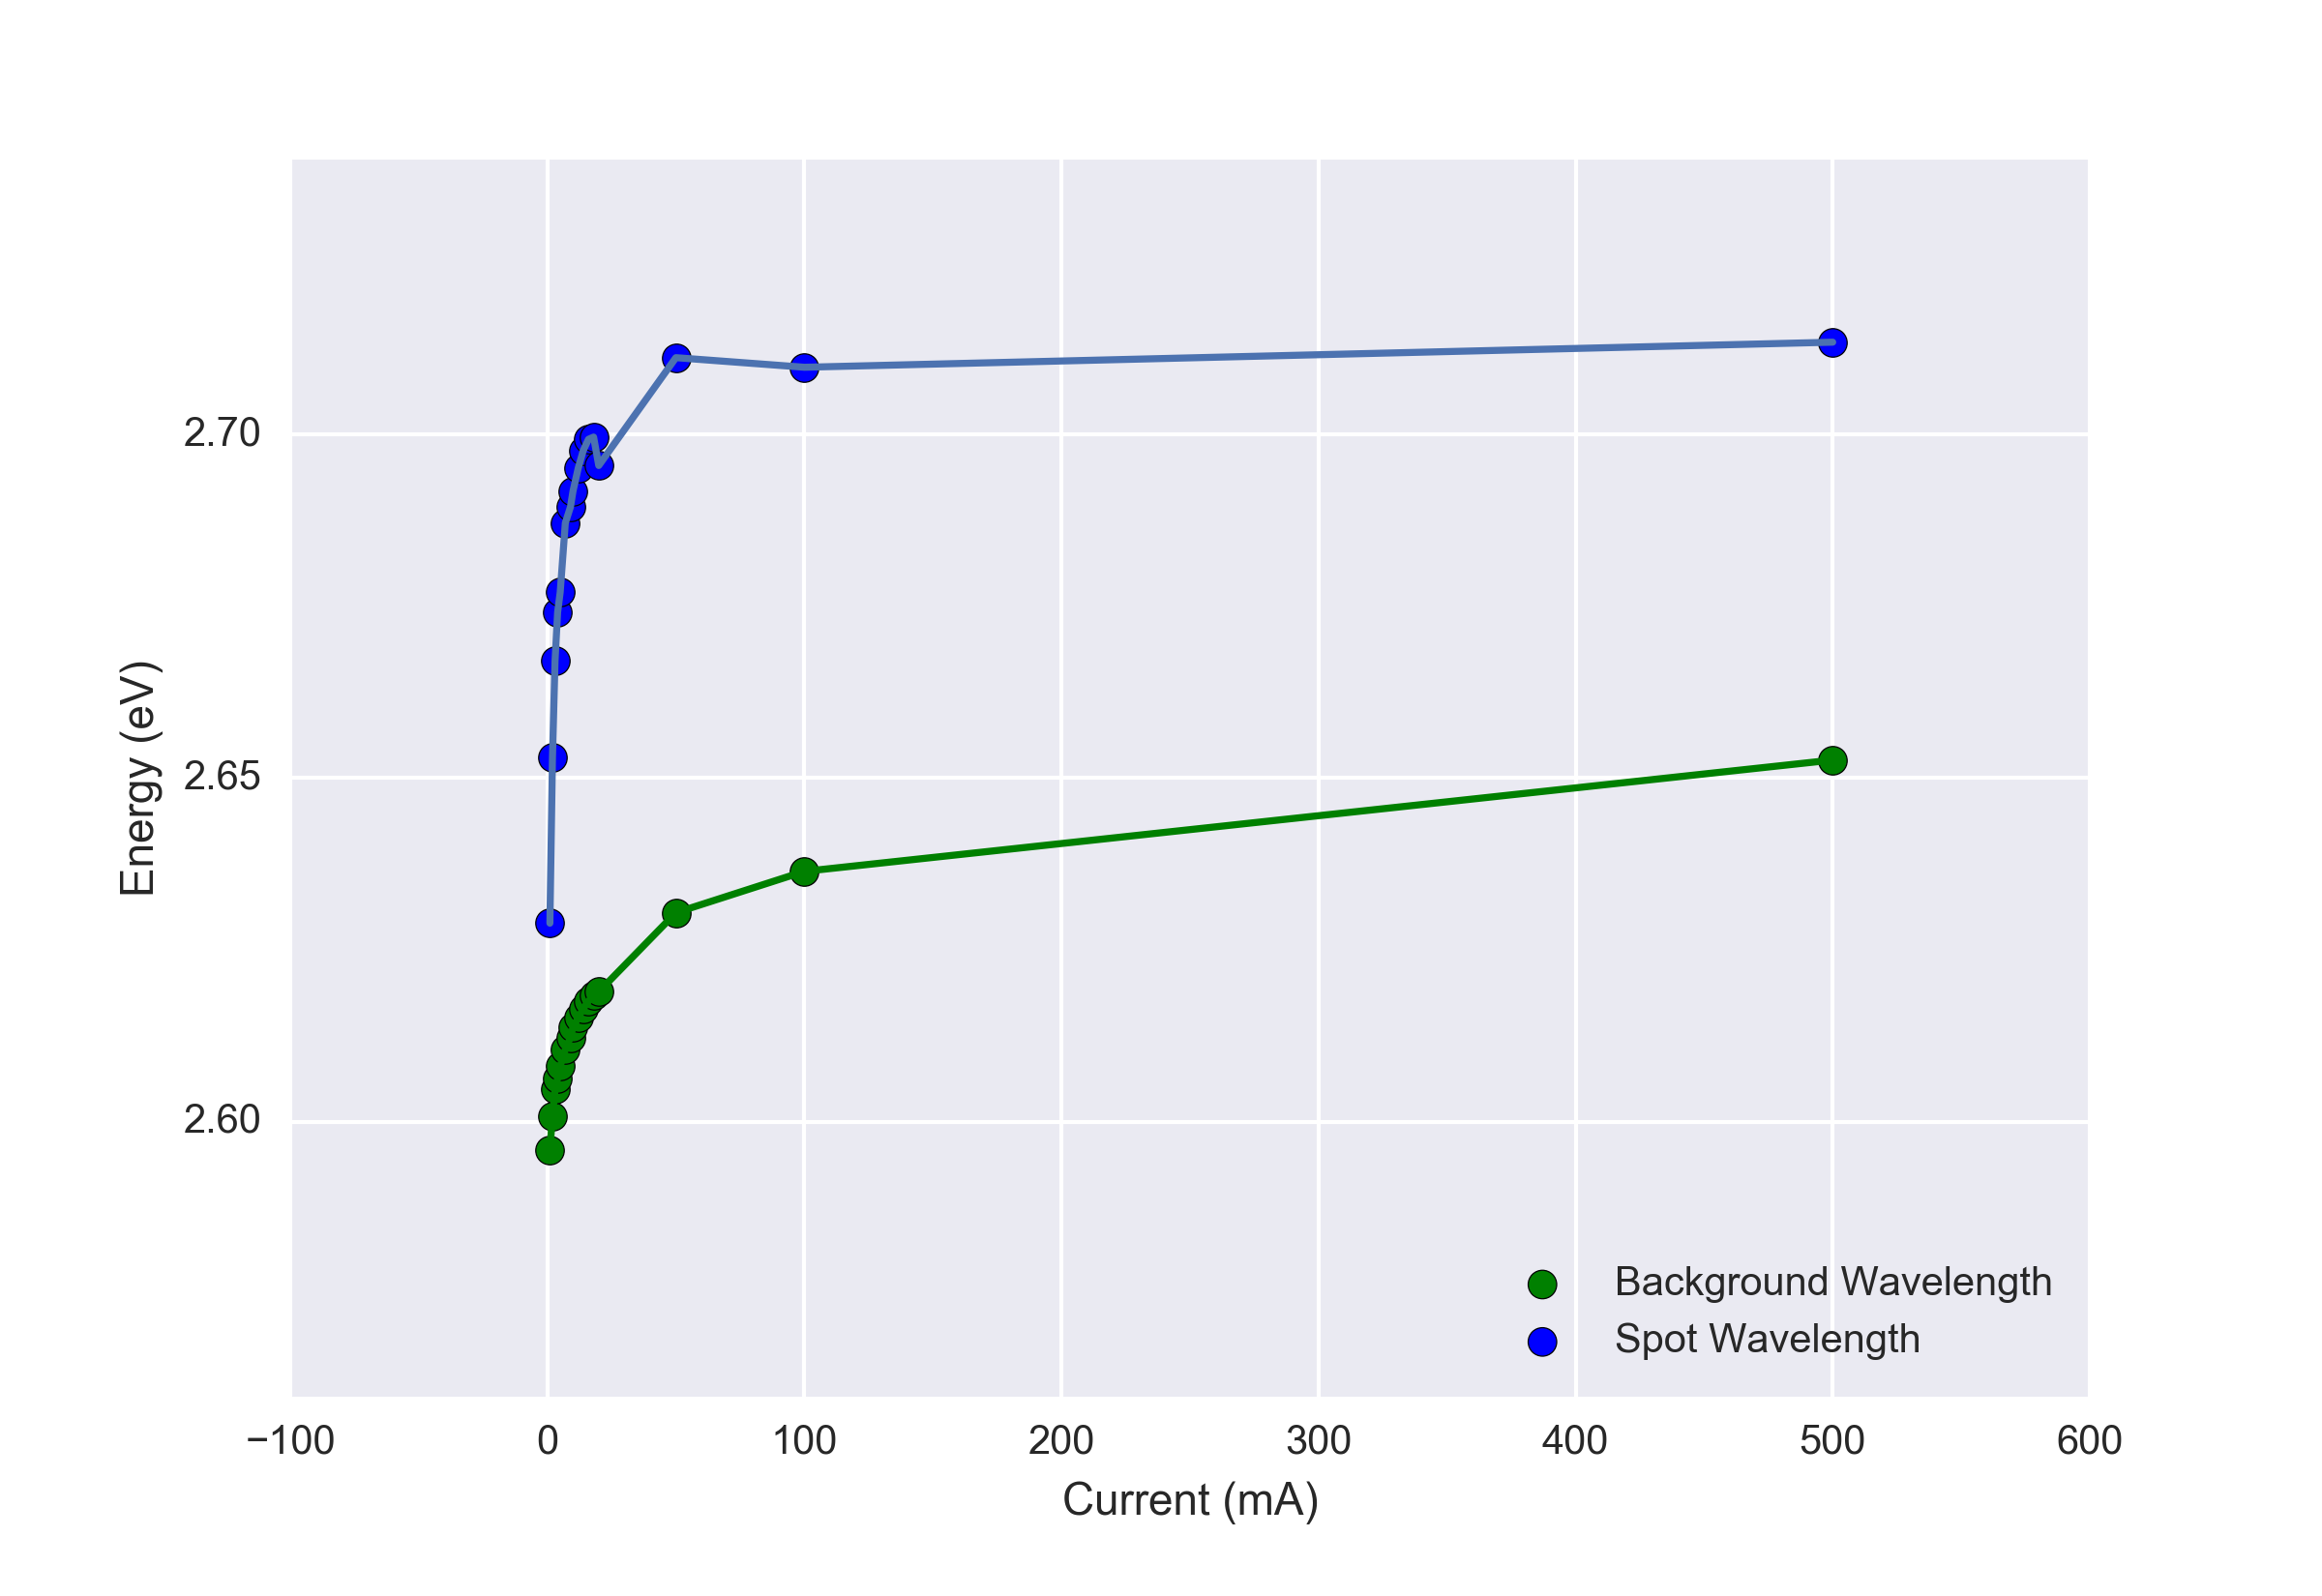
\includegraphics[width=0.8\textwidth]{Figs/Ch3/CentercompeV.png}
	\caption[h] {Spot and background average peak energy against injection current}
	\label{5610centrecomp}
\end{figure}

\FloatBarrier 

Device C5608A exhibited a similar current dependent relationship between the inhomogeneities and the background, as shown in Fig. \ref{5608peak} and \ref{5608centre}. As evidenced by Fig. \ref{probe}, Fig. \ref{5608peak} demonstrates a larger difference in EL intensity between the background and the inhomogeneities for C5608A relative to C5610A.

\begin{figure}[!ht]
	\centering
	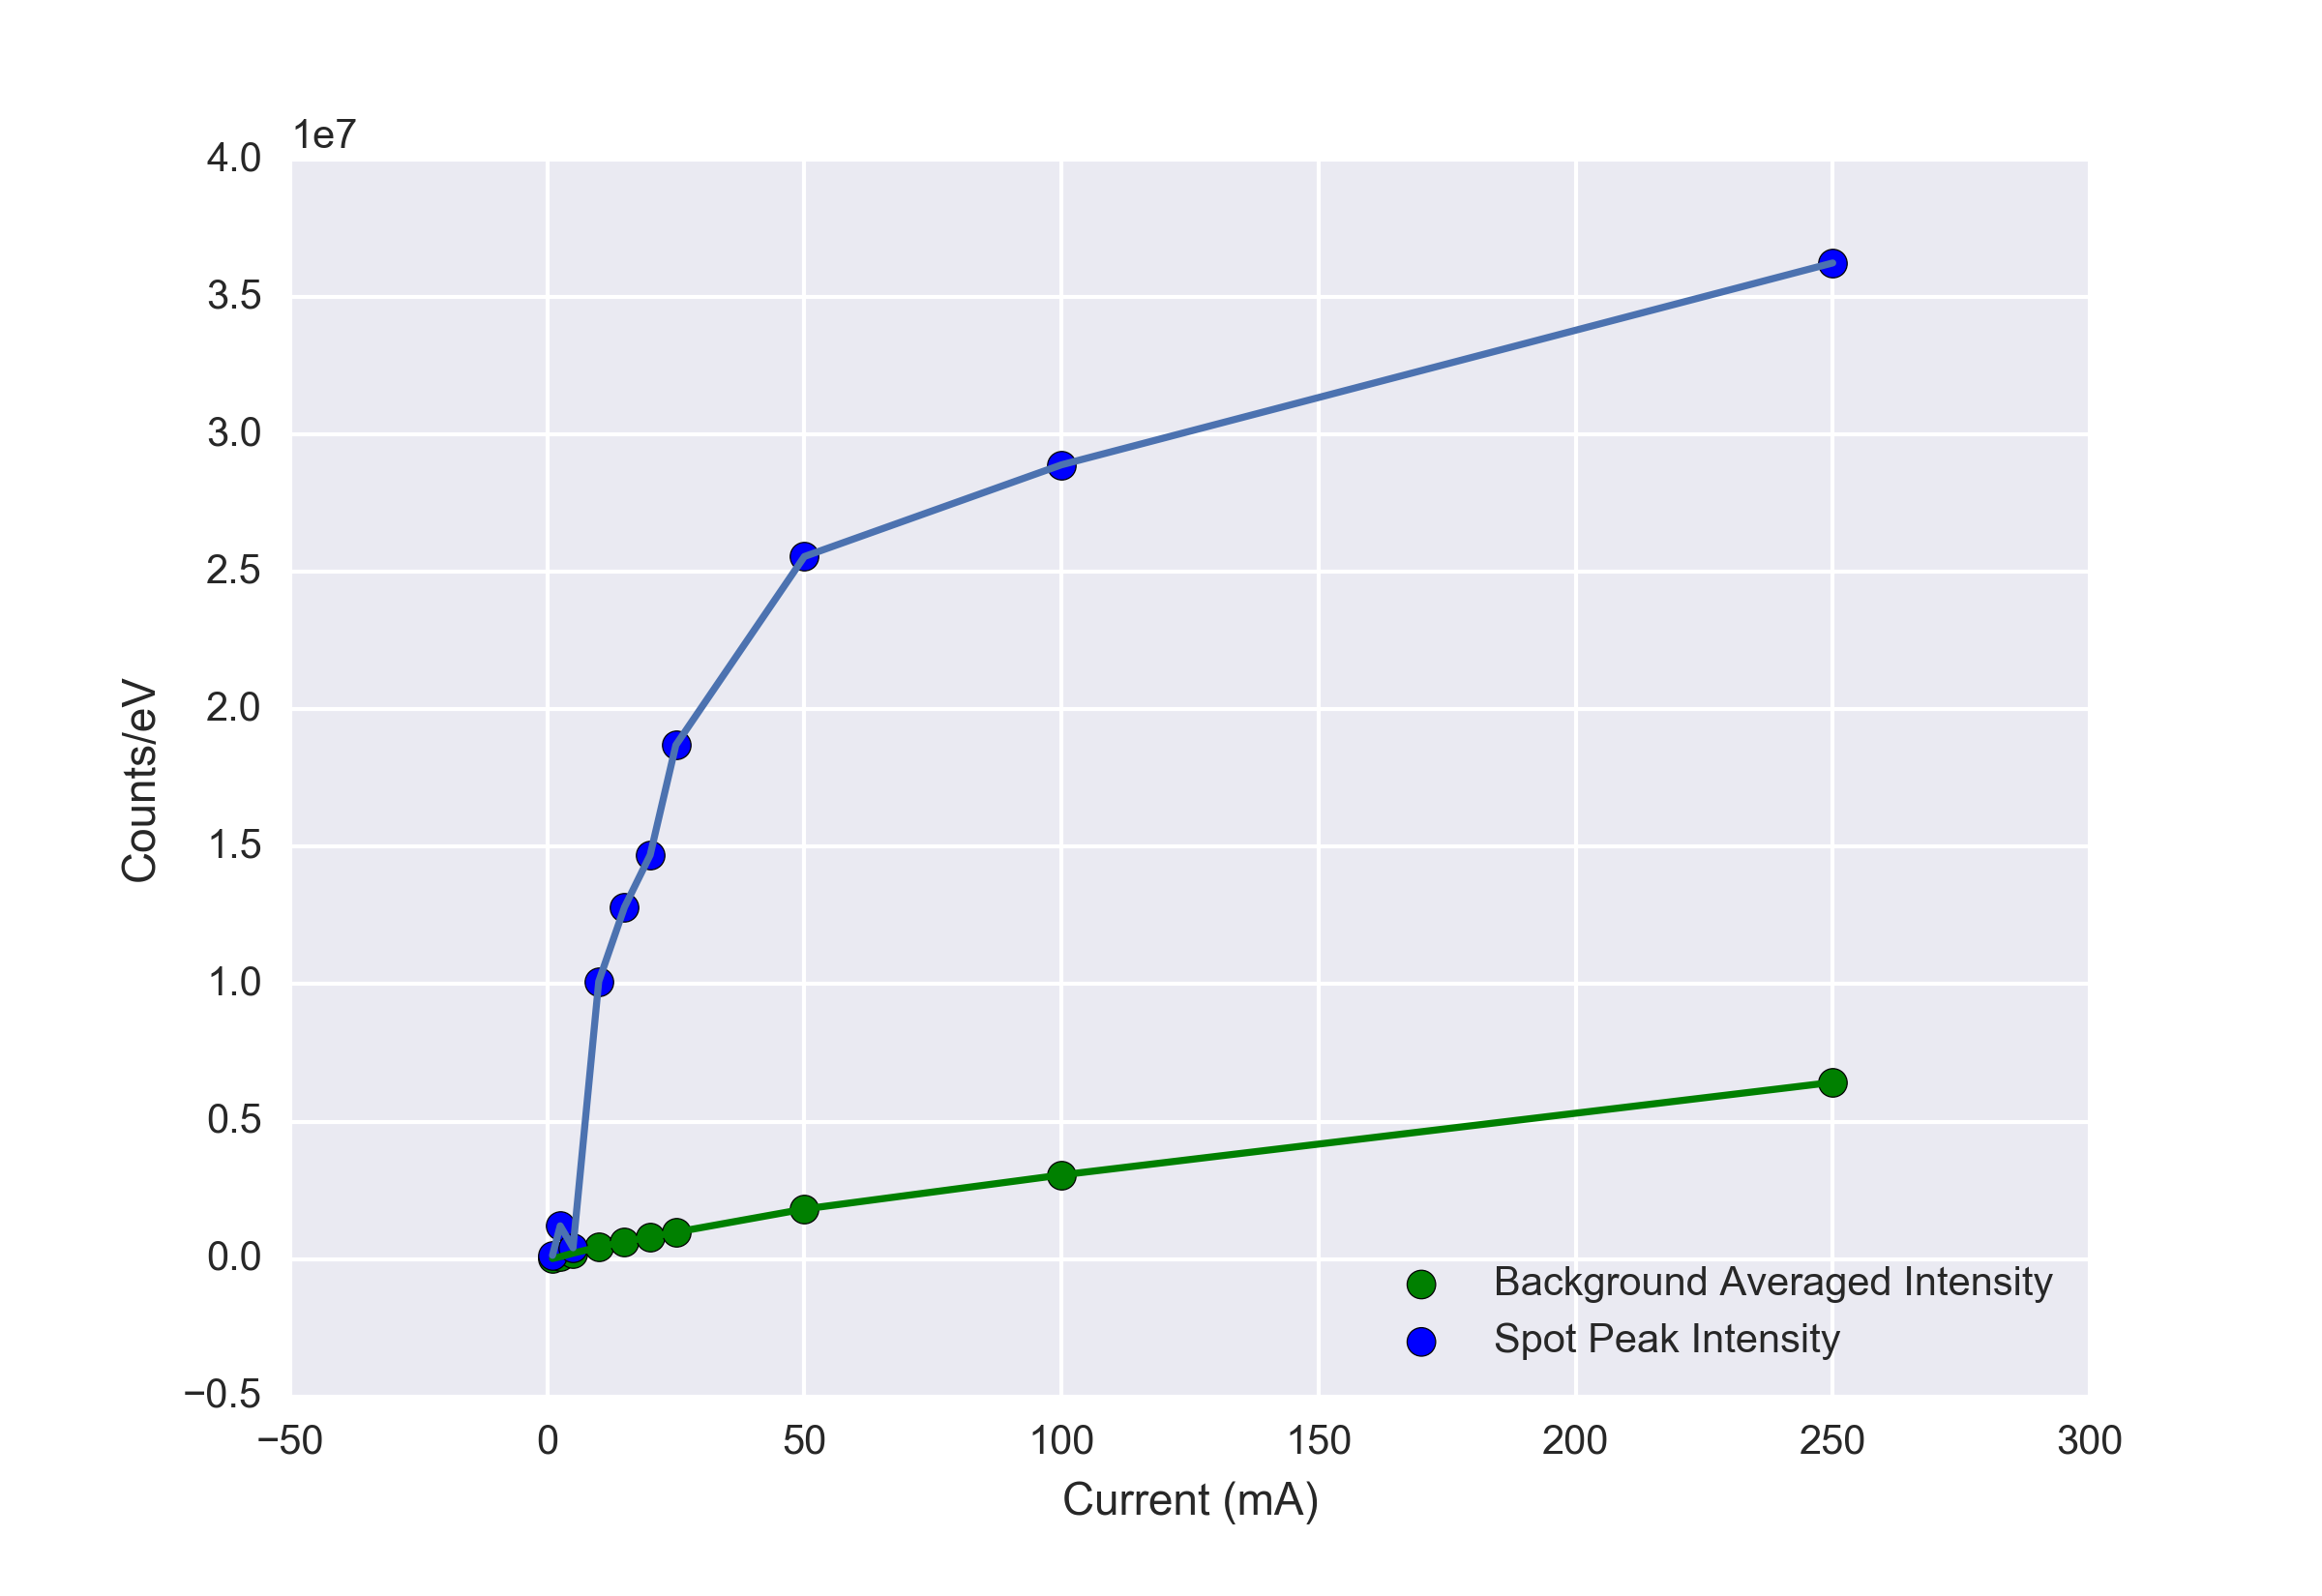
\includegraphics[width=0.8\textwidth]{Figs/Ch3/Peakcomp5608.png}
	\caption[h] {Spot and background average peak intensity against injection current}
	\label{5608peak}
\end{figure}
\FloatBarrier 

\begin{figure}[!ht]
	\centering
	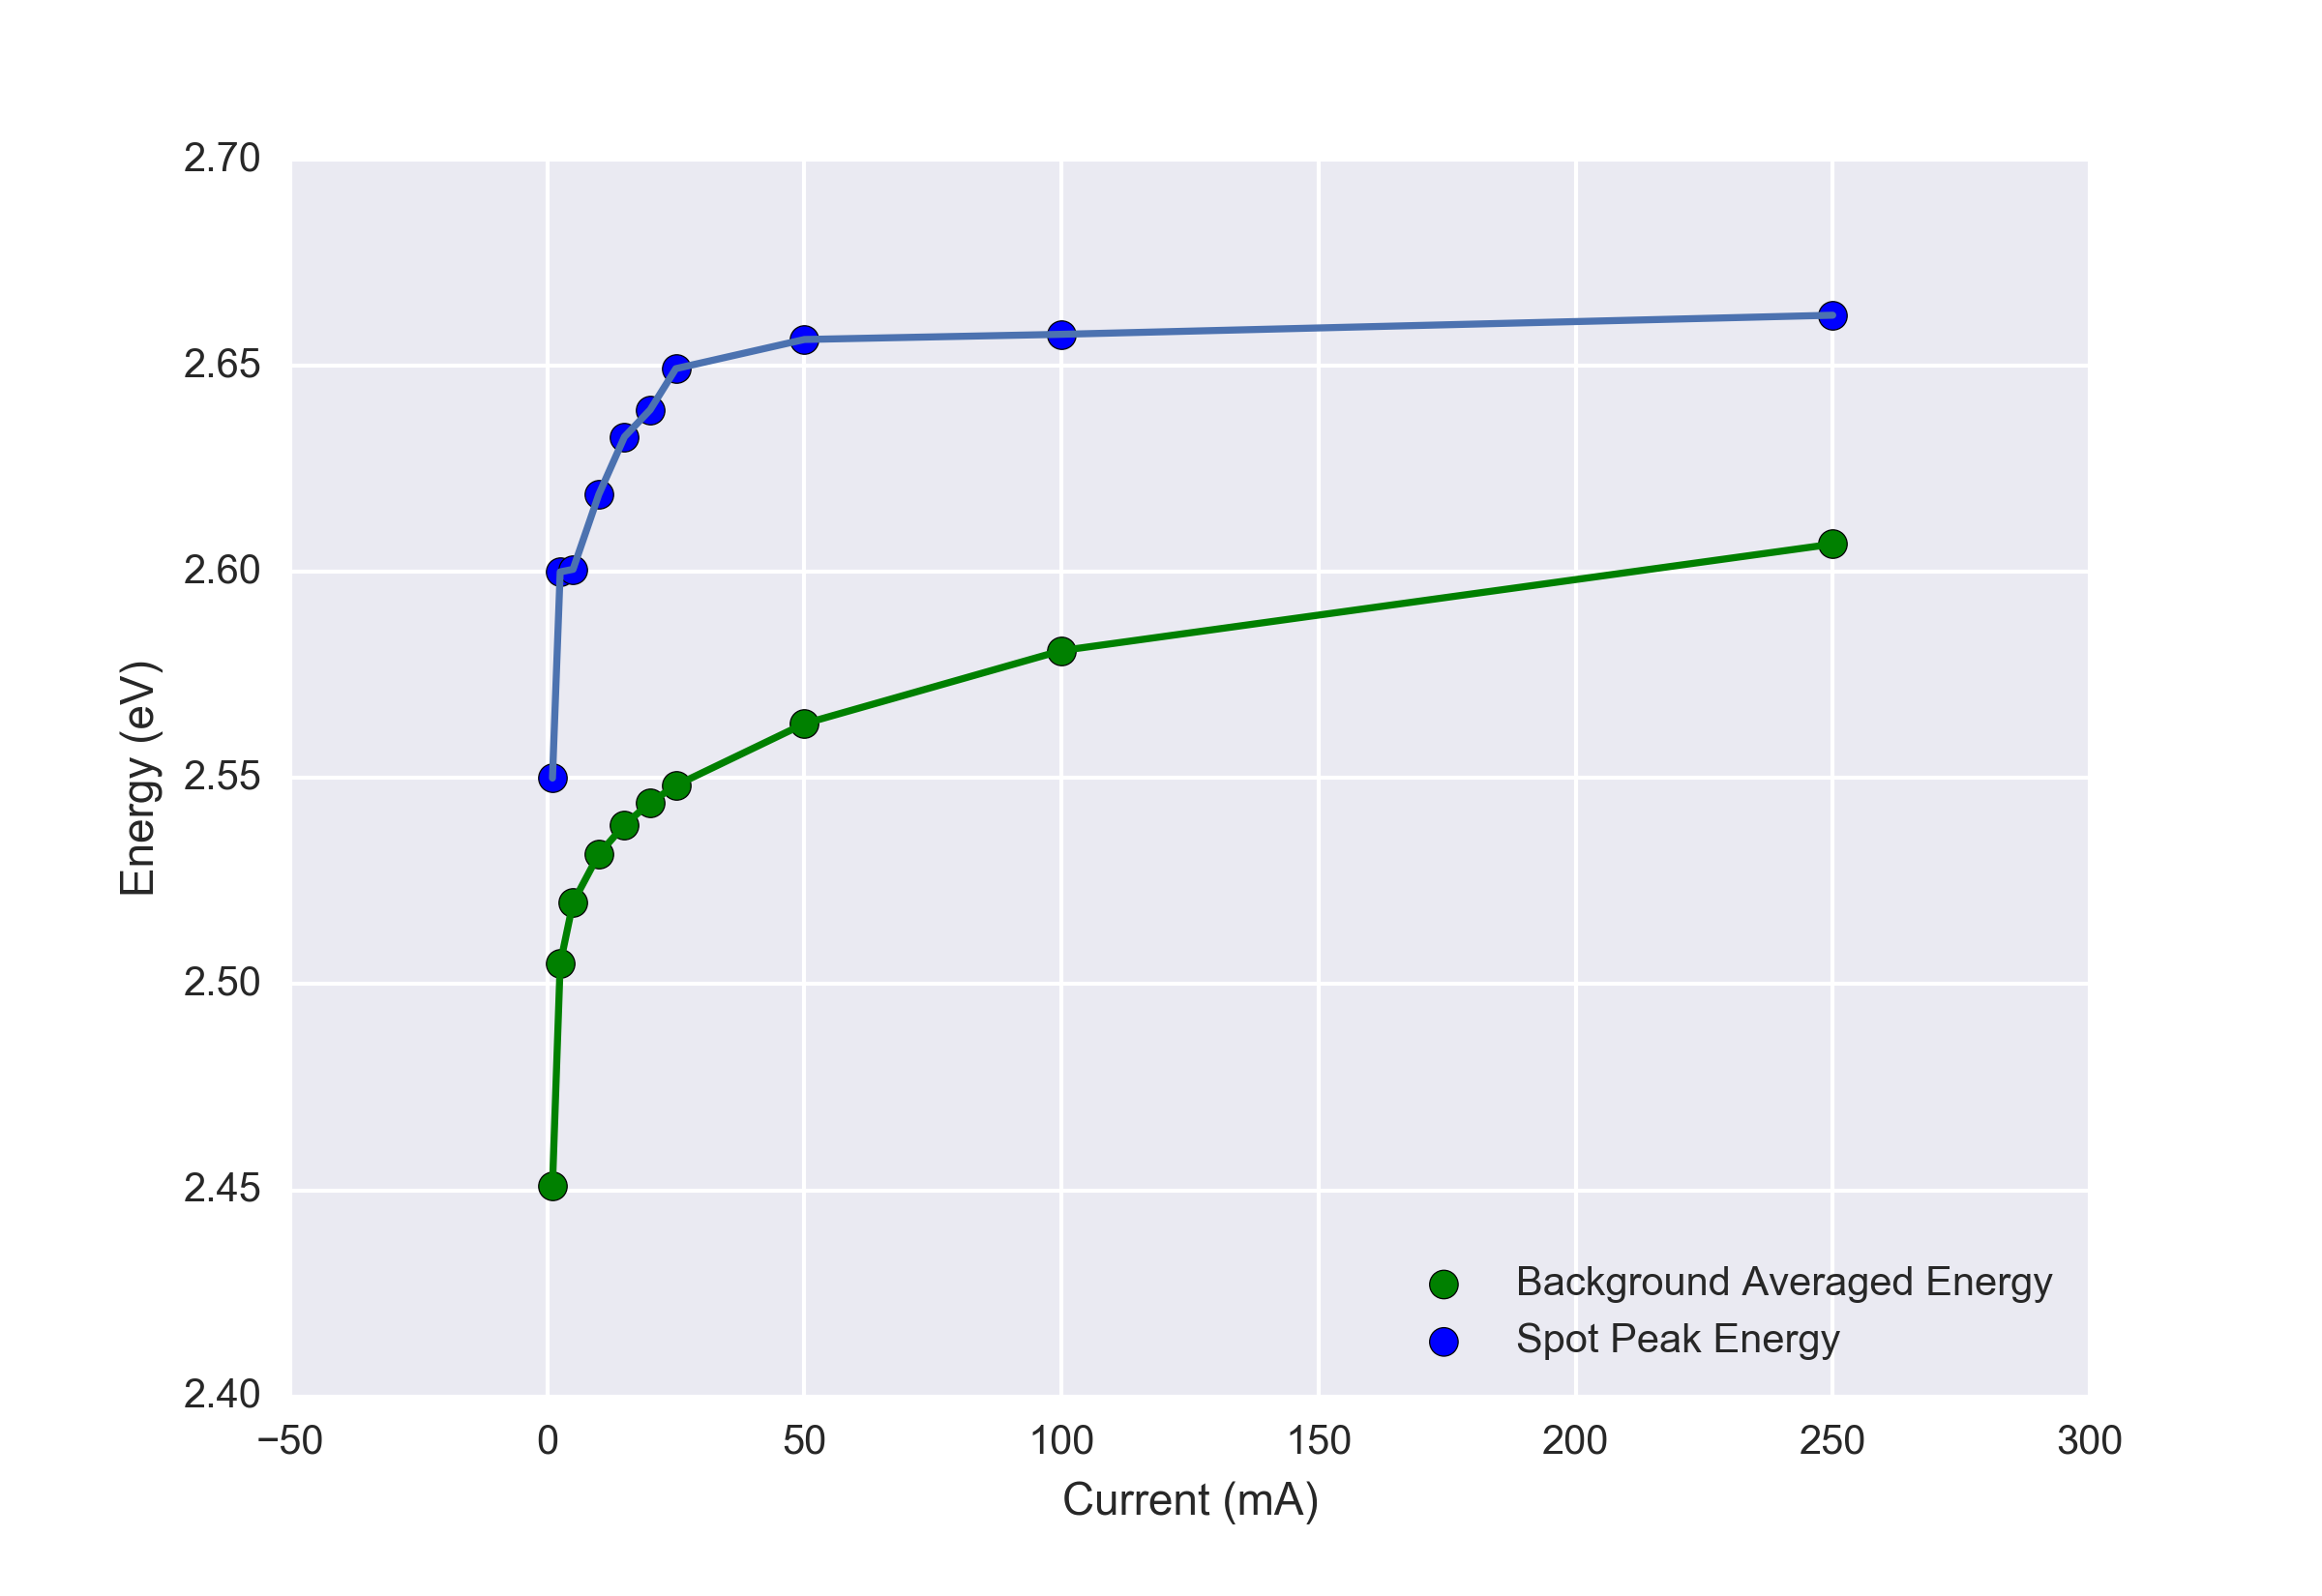
\includegraphics[width=0.8\textwidth]{Figs/Ch3/centrePeakcomp5608.png}
	\caption[h] {Spot and background average peak intensity against injection current}
	\label{5608centre}
\end{figure}
\FloatBarrier 

\subsection{Cathodoluminescence and Electron Beam Induced Current}
Having noted the behaviour of the inhomogeneities inferred from the hyperpsectral EL data, CL and EBIC data were taken over areas containing the inhomogeneities in order to examine their properties in more detail as CL and EBIC are electron beam based techniques and as such allow for a far higher resolution than EL mapping.\\
In order to achieve simultaneous CL and EBIC measurements, a Keithley Instrument 2401 source/measure unit was utilised in order to main the LED devices at a fixed bias of 0V thus allowing for the measurement of the short circuit current. During the CL image scanning, the Andor CCD camera was set-up to trigger the measure unit to record the current at each point in the CL spectral acquisition. The CL acquisition was performed with an electron beam at 10 kV and 1 nA. Unfortunately the secondary electron detector was inoperable during the acquisition of this data, as such there is no accompanying SEM micrograph for the CL and EBIC data. The CL and EBIC data for devices C5610A and C5608A are shown in figures \ref{5610CLEBIC} and \ref{5608CLEBIC} respectively.


\begin{figure}[h]
	\hspace*{0.5cm}
	\begin{subfigure}[b]{0.4\textwidth}
		\centering
		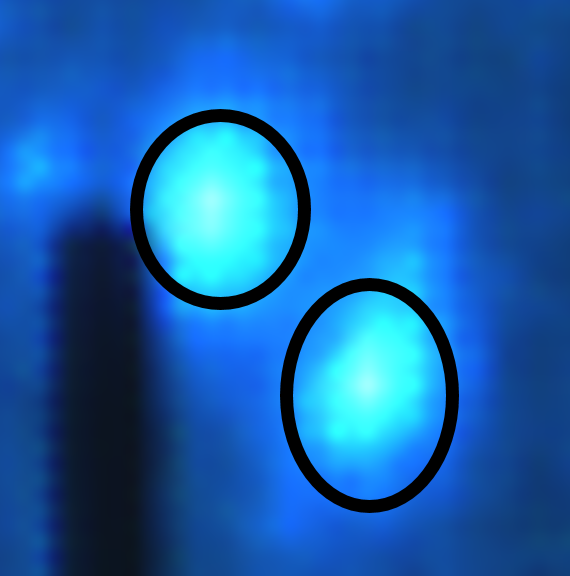
\includegraphics[width=0.7\linewidth]{Figs/Ch3/5610CLEBICloc}
		\caption{}
		
	\end{subfigure}%
	\hspace*{2cm}
	\begin{subfigure}[b]{0.4\textwidth}
		\centering
		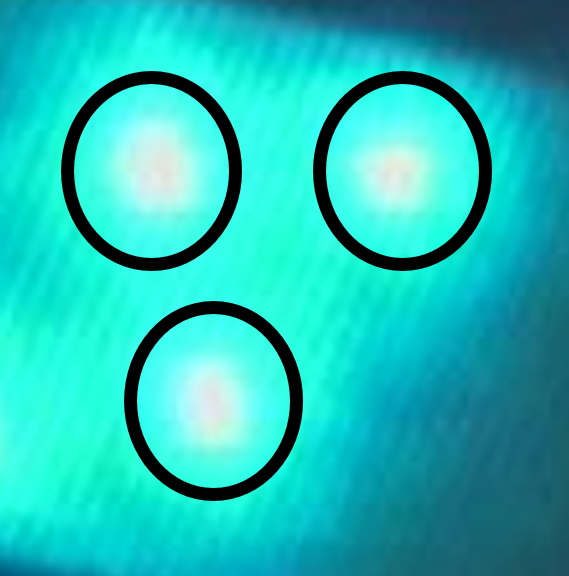
\includegraphics[width=0.7\linewidth]{Figs/Ch3/5608CLEBICloc}
		\caption{}
	\end{subfigure}%
	
	\caption{EL images of the regions examined using CL and EBIC mapping for a) C5610A and b) C5608A.}
	\label{5610loc}
\end{figure}

\FloatBarrier
\begin{figure}[h]
	\hspace*{0.5cm}
	\begin{subfigure}[b]{0.48\textwidth}
		\centering
		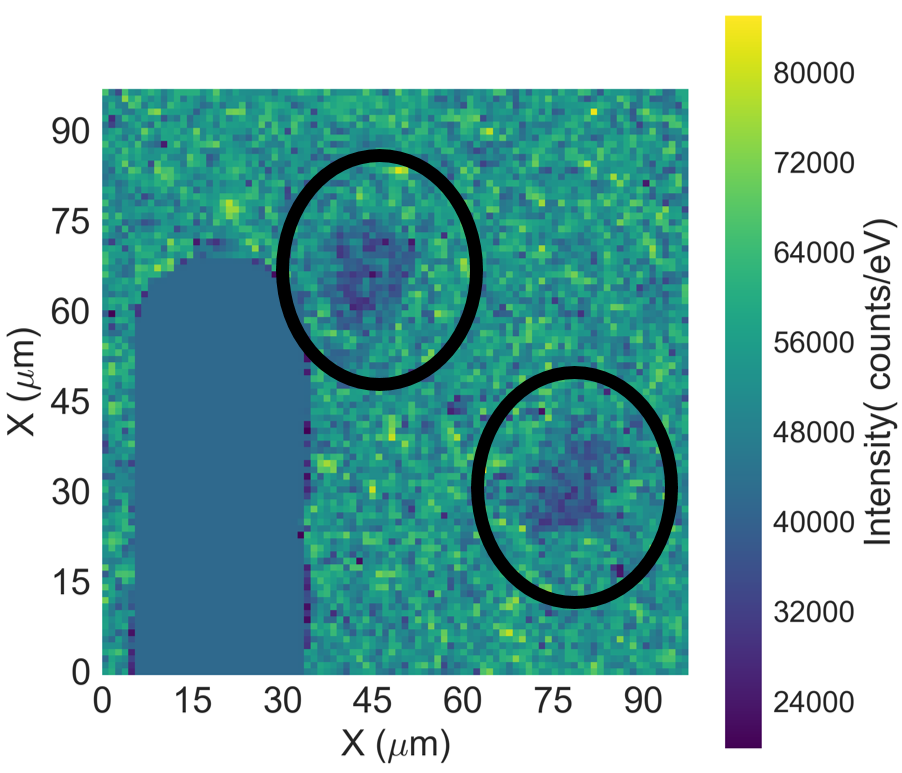
\includegraphics[width=1\linewidth]{Figs/Ch3/5610AsmallCL}
		\caption{}
		
	\end{subfigure}%
	\hspace*{0.5cm}
	\begin{subfigure}[b]{0.48\textwidth}
		\centering
		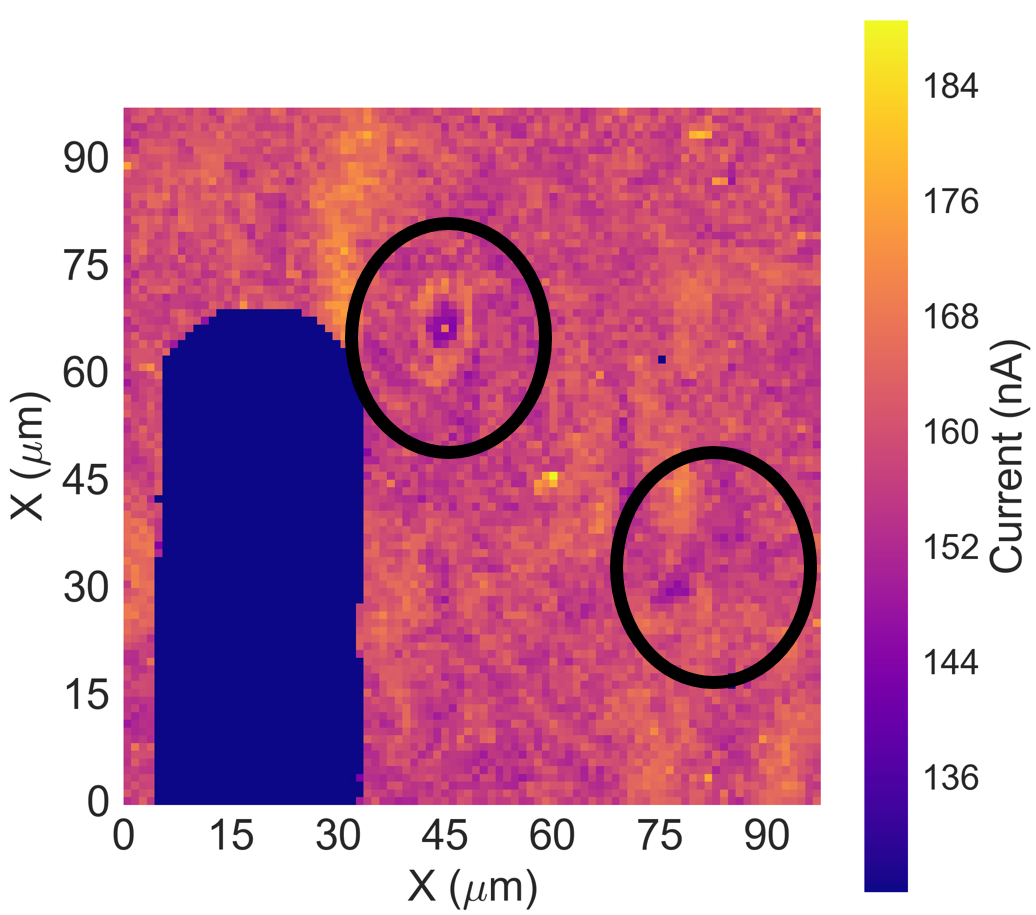
\includegraphics[width=0.98\linewidth]{Figs/Ch3/5610smallEBIC}
		\caption{}
	\end{subfigure}%
	
	\caption{a) CL and b) EBIC maps acquired simultaneously of the area shown in Fig.\ref{5610loc} a.}
	\label{5610CLEBIC}
\end{figure}

\FloatBarrier

\begin{figure}[h]
	\hspace*{0.5cm}
	\begin{subfigure}[b]{0.48\textwidth}
		\centering
		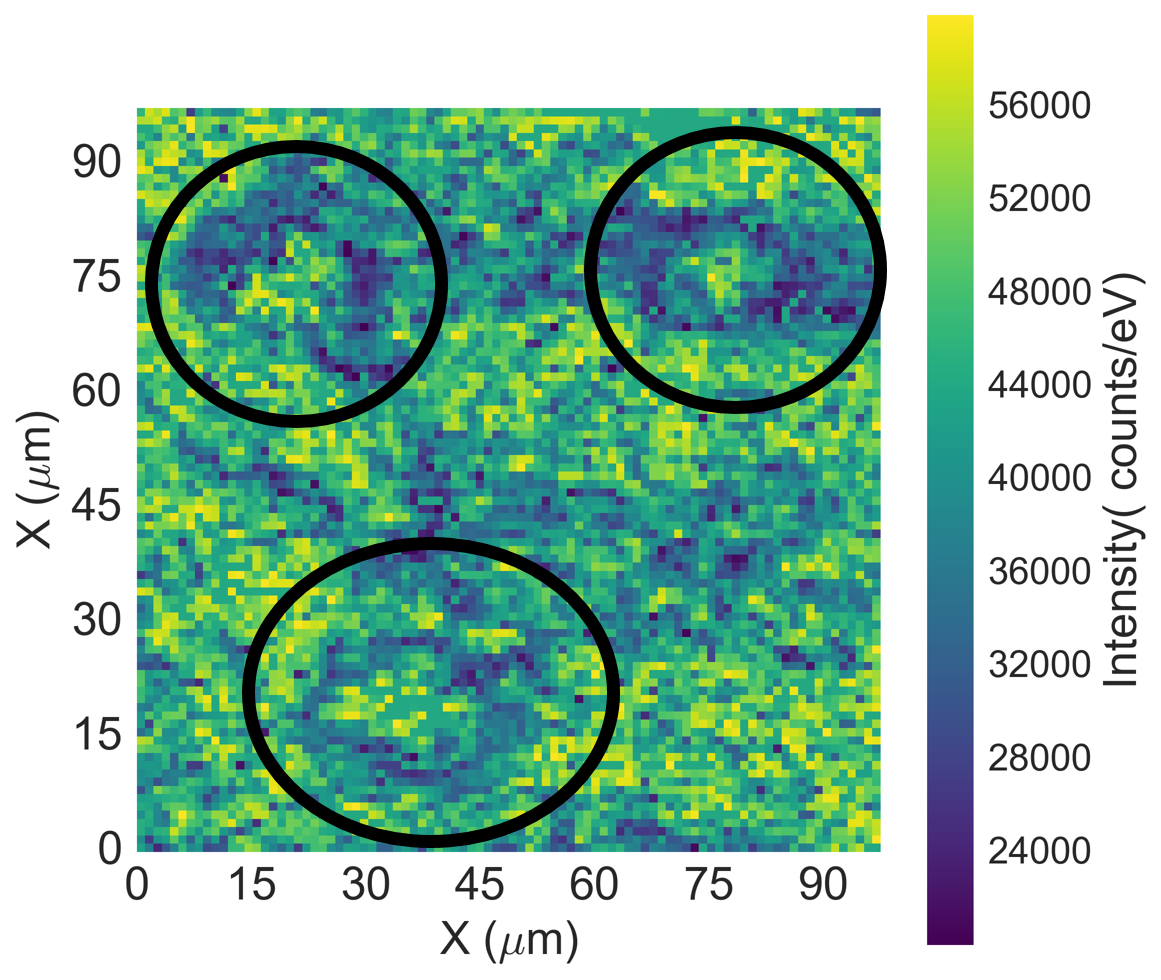
\includegraphics[width=1\linewidth]{Figs/Ch3/5608AsmallCL}
		\caption{}
		
	\end{subfigure}%
	\hspace*{0.5cm}
	\begin{subfigure}[b]{0.48\textwidth}
		\centering
		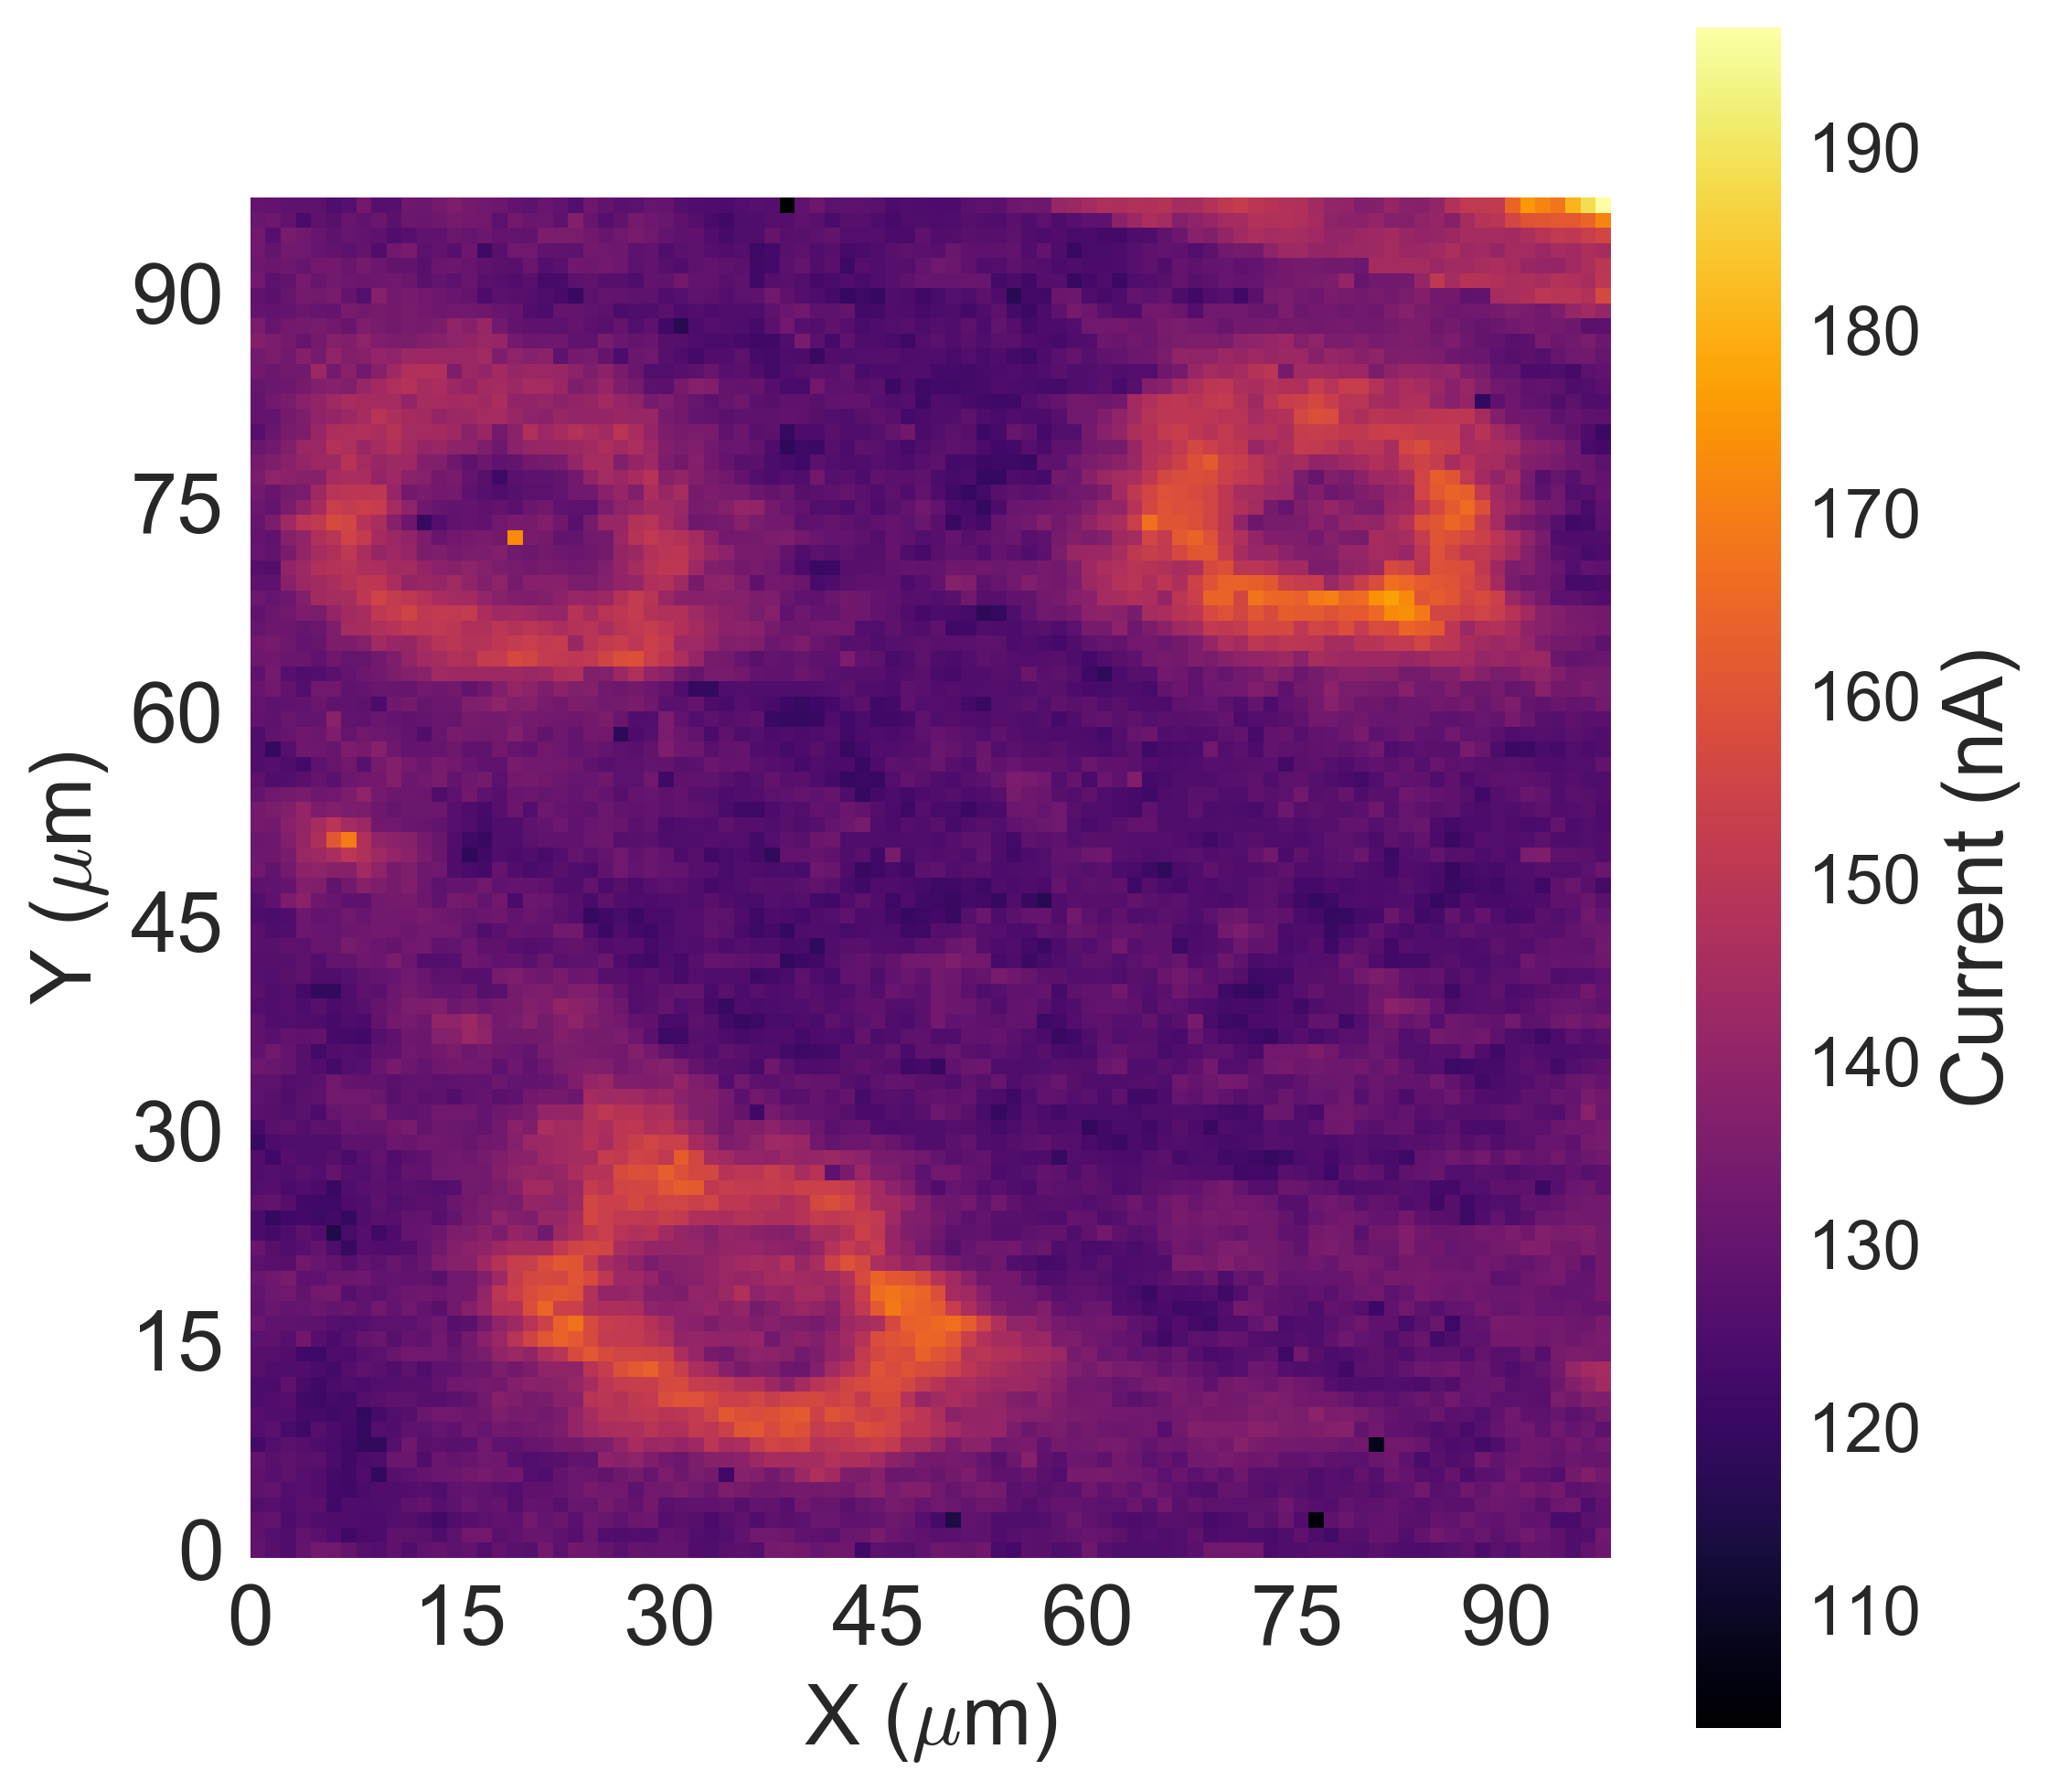
\includegraphics[width=0.98\linewidth]{Figs/Ch3/5608smallEBIC}
		\caption{}
	\end{subfigure}%
	
	\caption{a) CL and b) EBIC maps acquired simultaneously of the area shown in Fig.\ref{5610loc}b.}
	\label{5608CLEBIC}
\end{figure}
\FloatBarrier

Fig. \ref{5610CLEBIC}a. shows the inhomogeneities exhibit a lower CL intensity relative to the background, in contrast to the EL. Interestingly, the EBIC signal, shown in Fig.\ref{5610CLEBIC} for both inhomogeneities examined seem rather different. The feature closest to the contact region can be seen as a region of high EBIC surrounding a region of lower extracted current. However the feature furthest from the electrical contact shows far less prominent EBIC signal.\\
The features examined are far more prominent in the case of device C5608A. Fig.\ref{5608CLEBIC}.a. shows the detection of 'rings' emitting at a lower at a lower intensity in the CL at the location of the features. These rings correspond to rings of higher EBIC current as observed in Fig.\ref{5608CLEBIC}.b.

\subsubsection{Scanning Electron Microscopy with Cathodoluminescence}
Following the CL and EBIC scans shown in figures \ref{5610CLEBIC} and \ref{5608CLEBIC} performed at Strathclyde University, more detailed SEM-CL experiments were performed at the University of Cambridge using a Phillips XL30s field emission SEM equipped with a Gatan MonoCL4 system to record the CL signal. This set-up provides the additional benefit of panchromatic CL imaging, which allows for the detection of the features without the need for extremely detailed EL correlation.

\begin{figure}[h]
	
	\begin{subfigure}[b]{0.48\textwidth}
		\centering
		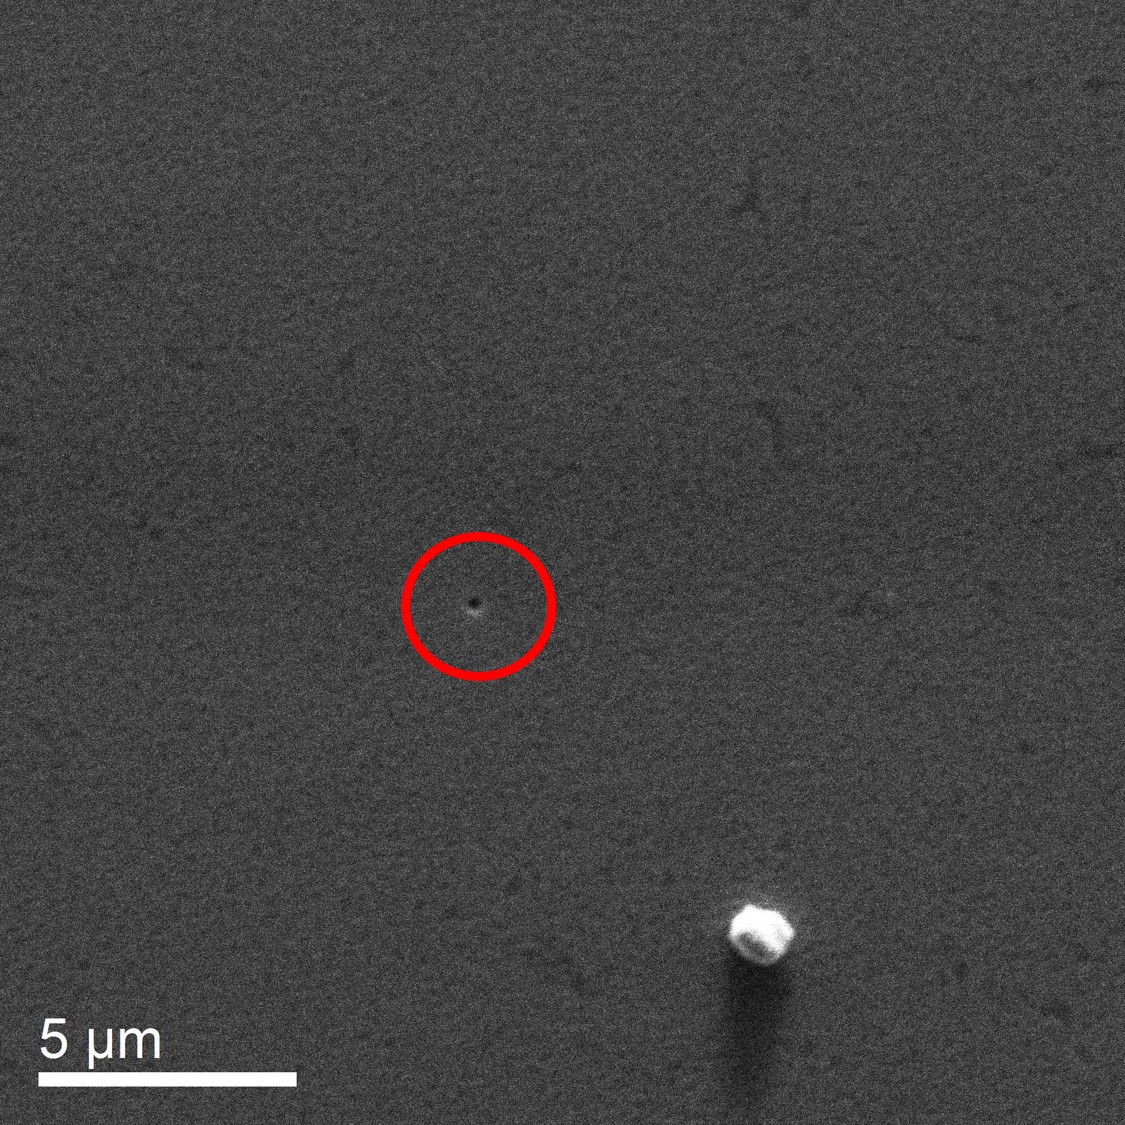
\includegraphics[width=0.7\linewidth]{Figs/Ch3/5610sem}
		\caption{}
		
	\end{subfigure}%
	\hspace*{0.5cm}
	\begin{subfigure}[b]{0.48\textwidth}
		\centering
		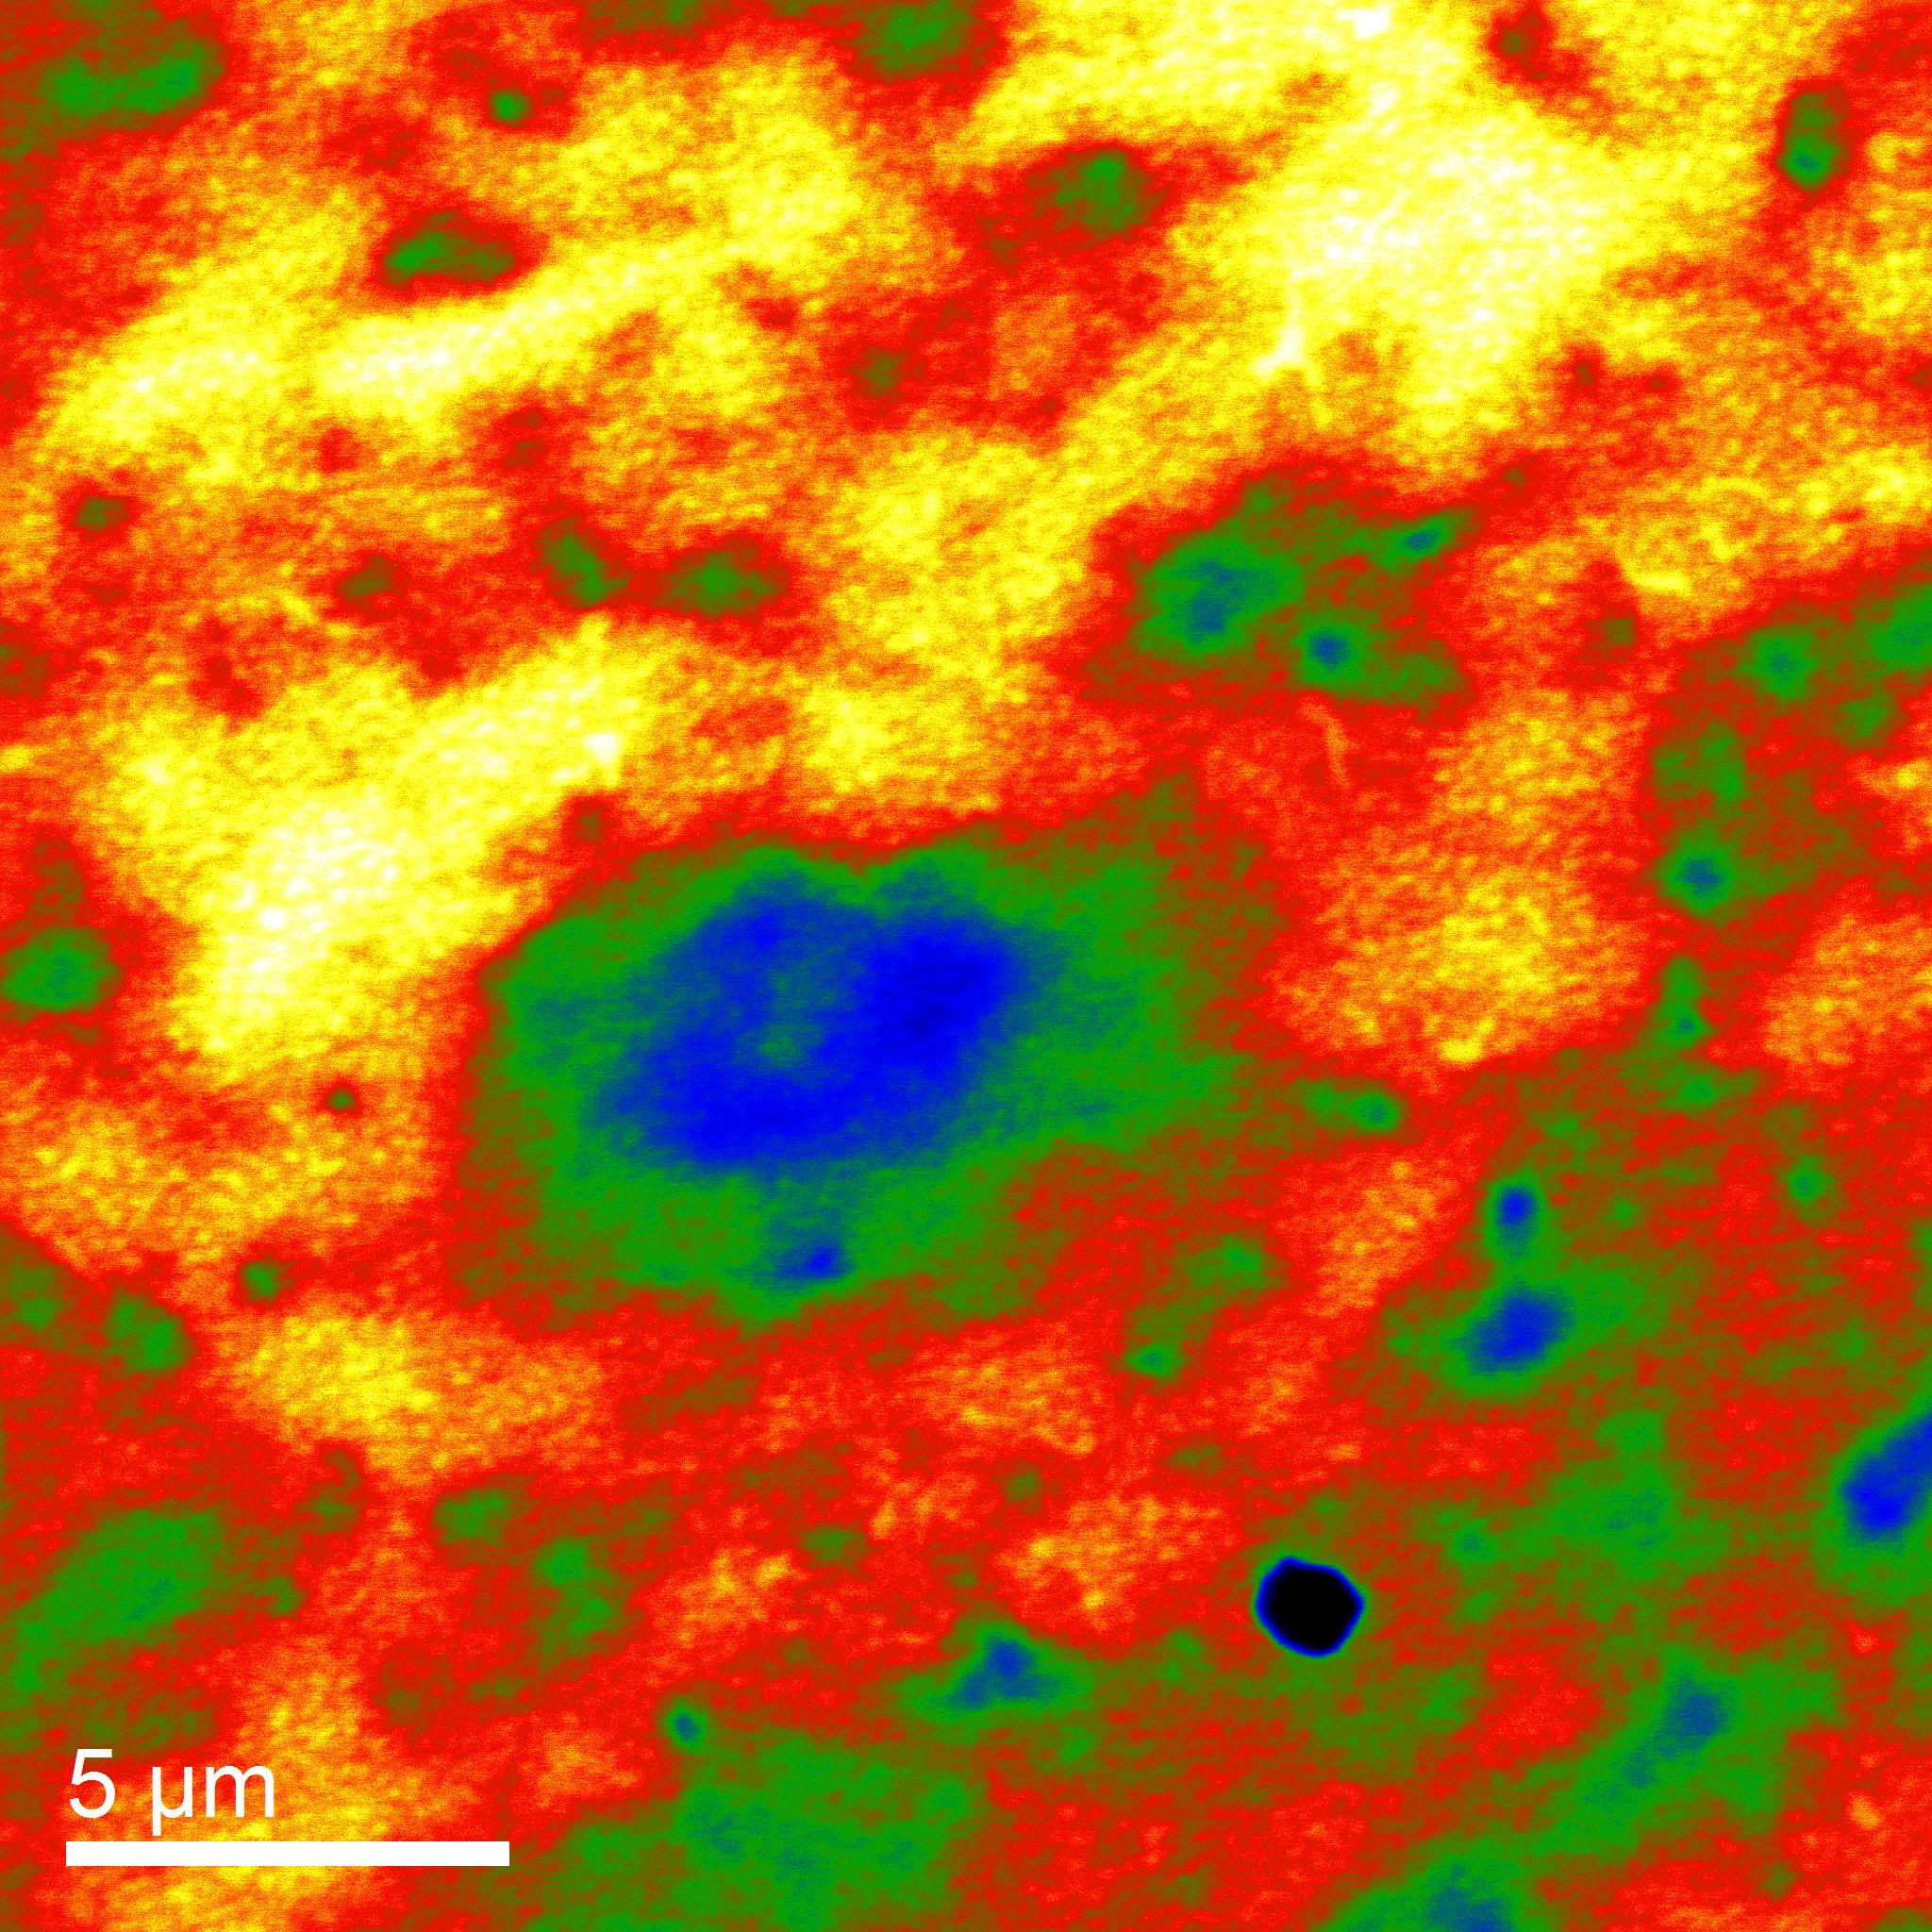
\includegraphics[width=0.7\linewidth]{Figs/Ch3/5610panCL}
		\caption{}
	\end{subfigure}%
	
	\caption{a) SEM micrograph and b) pan-CL image of an inhomogeneity in C5610A. The pan-CL image utilises a temperature scale (blue = low, red = high).}
	\label{5610-SEM-CL}
\end{figure}
\FloatBarrier

\begin{figure}[h]
	
	\begin{subfigure}[b]{0.48\textwidth}
		\centering
		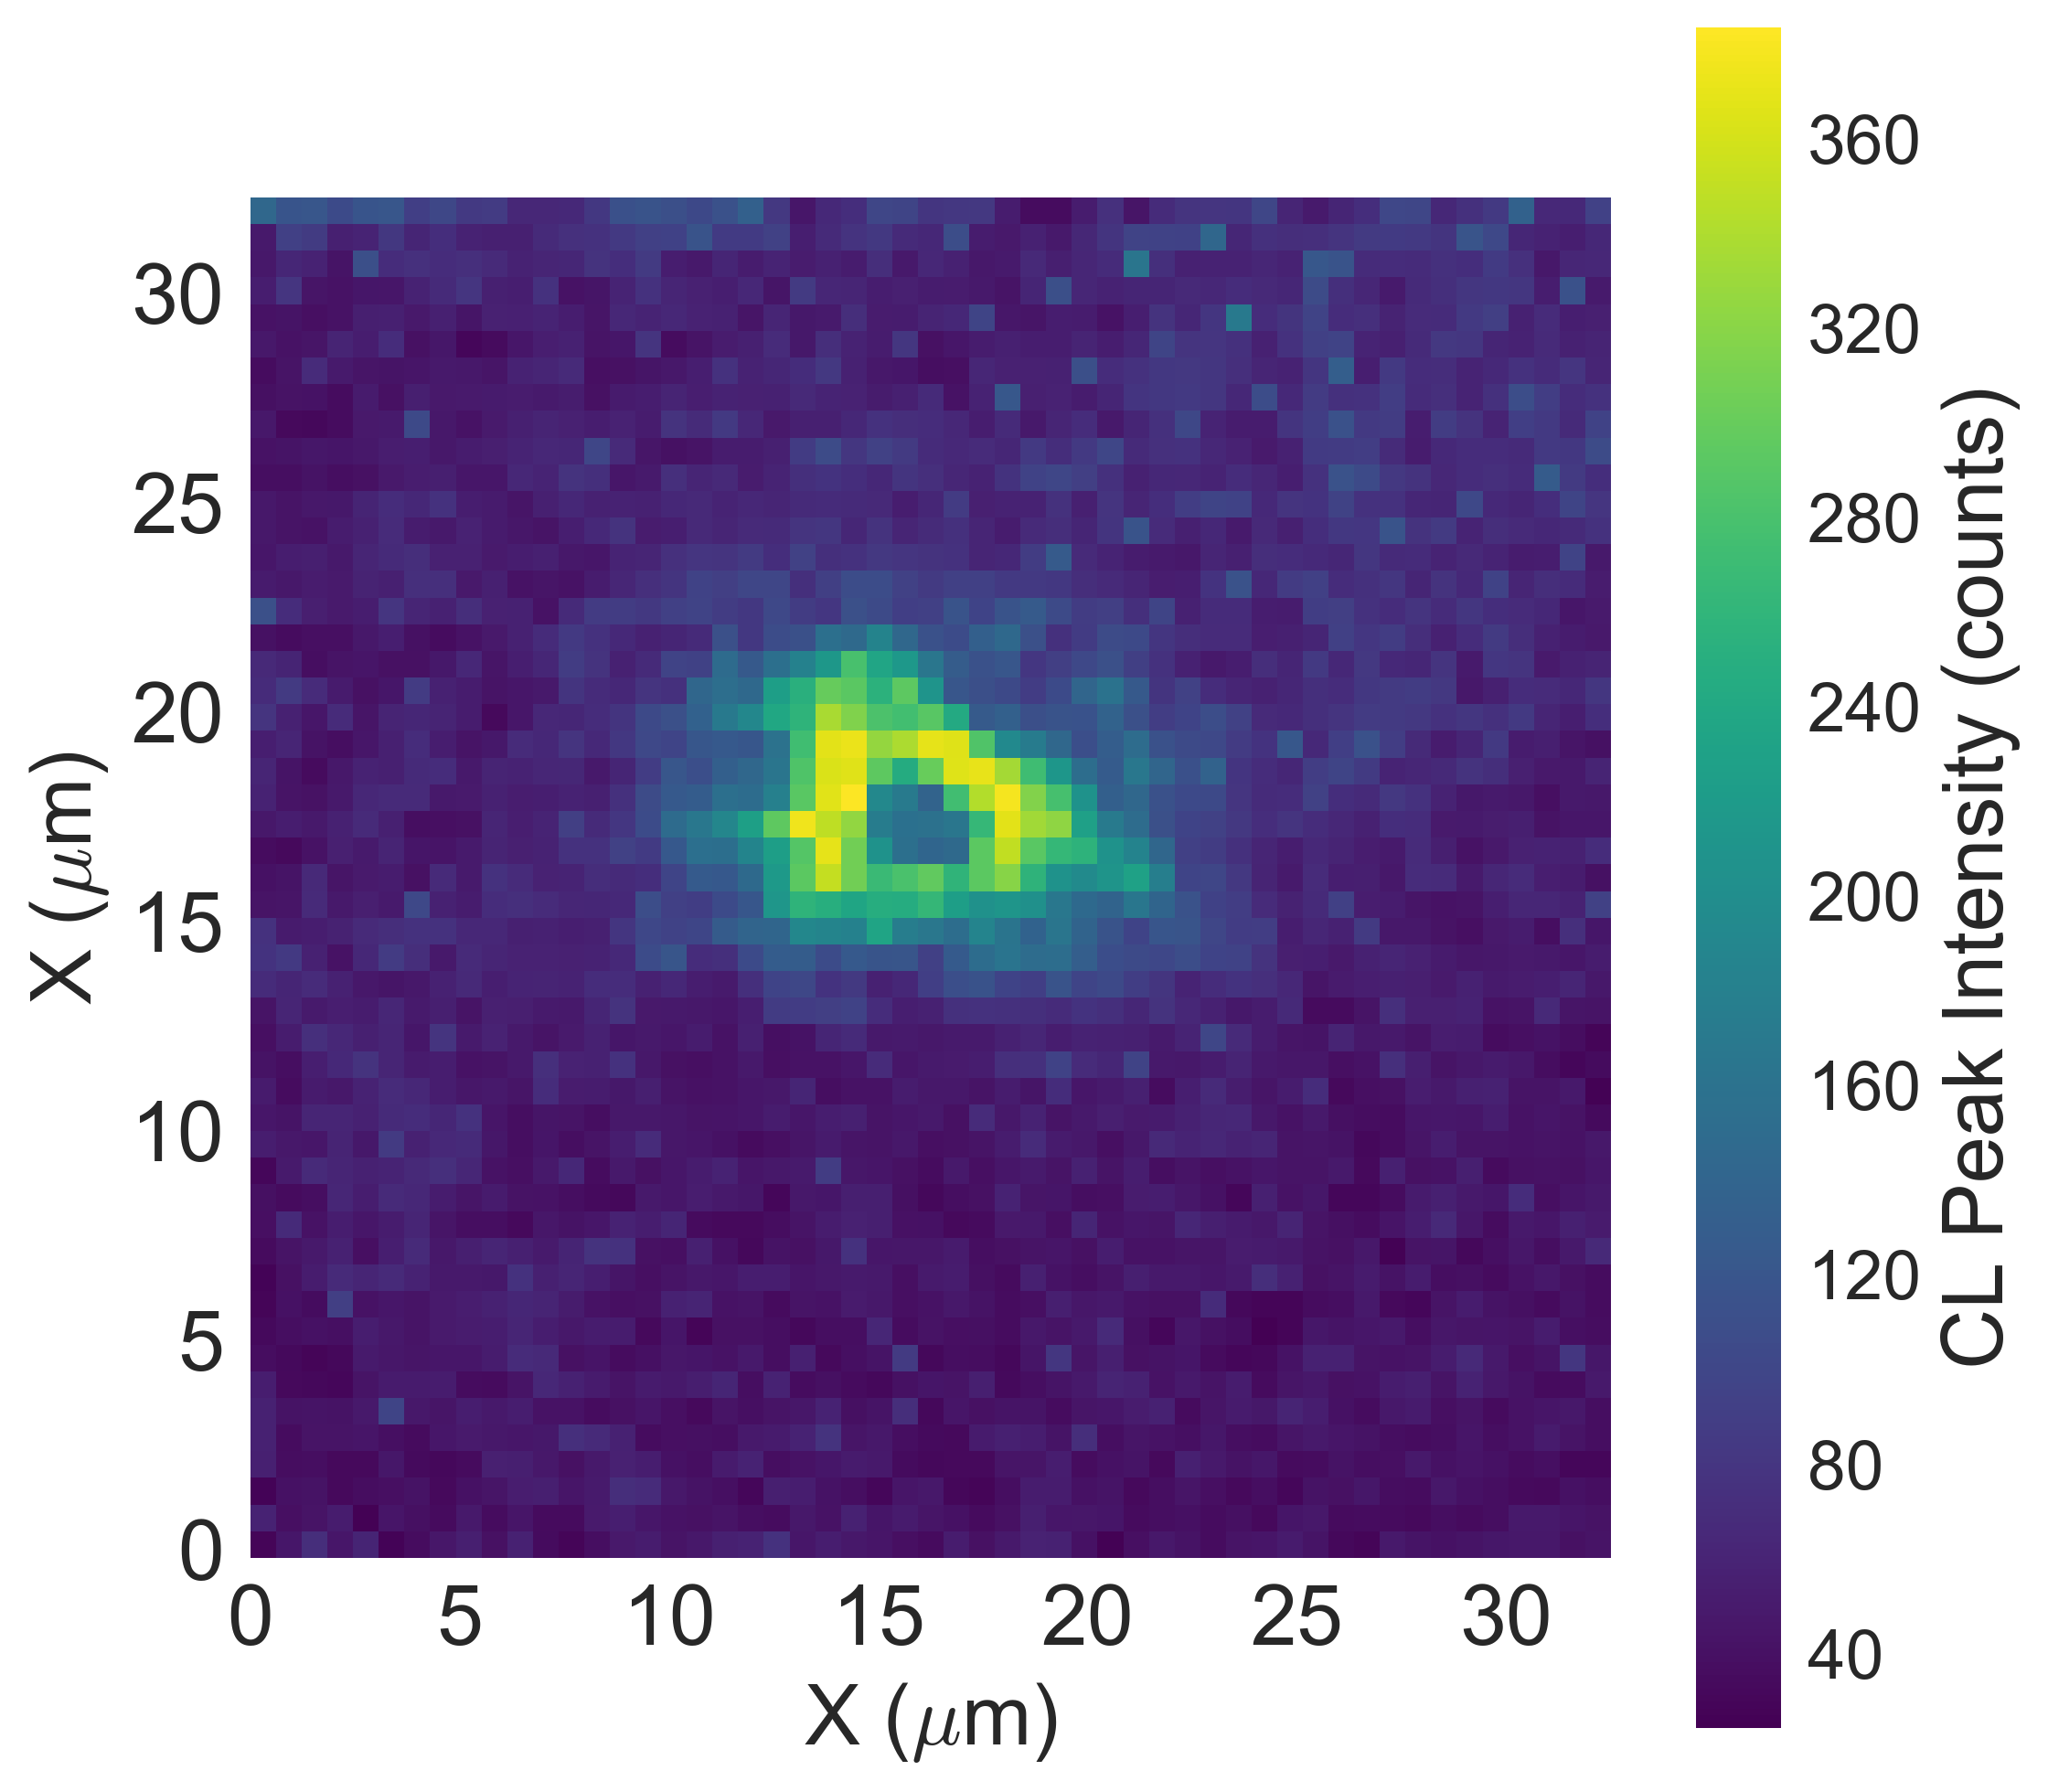
\includegraphics[width=1\linewidth]{Figs/Ch3/A-peak}
		\caption{}
		
	\end{subfigure}%
	\hspace*{0.5cm}
	\begin{subfigure}[b]{0.48\textwidth}
		\centering
		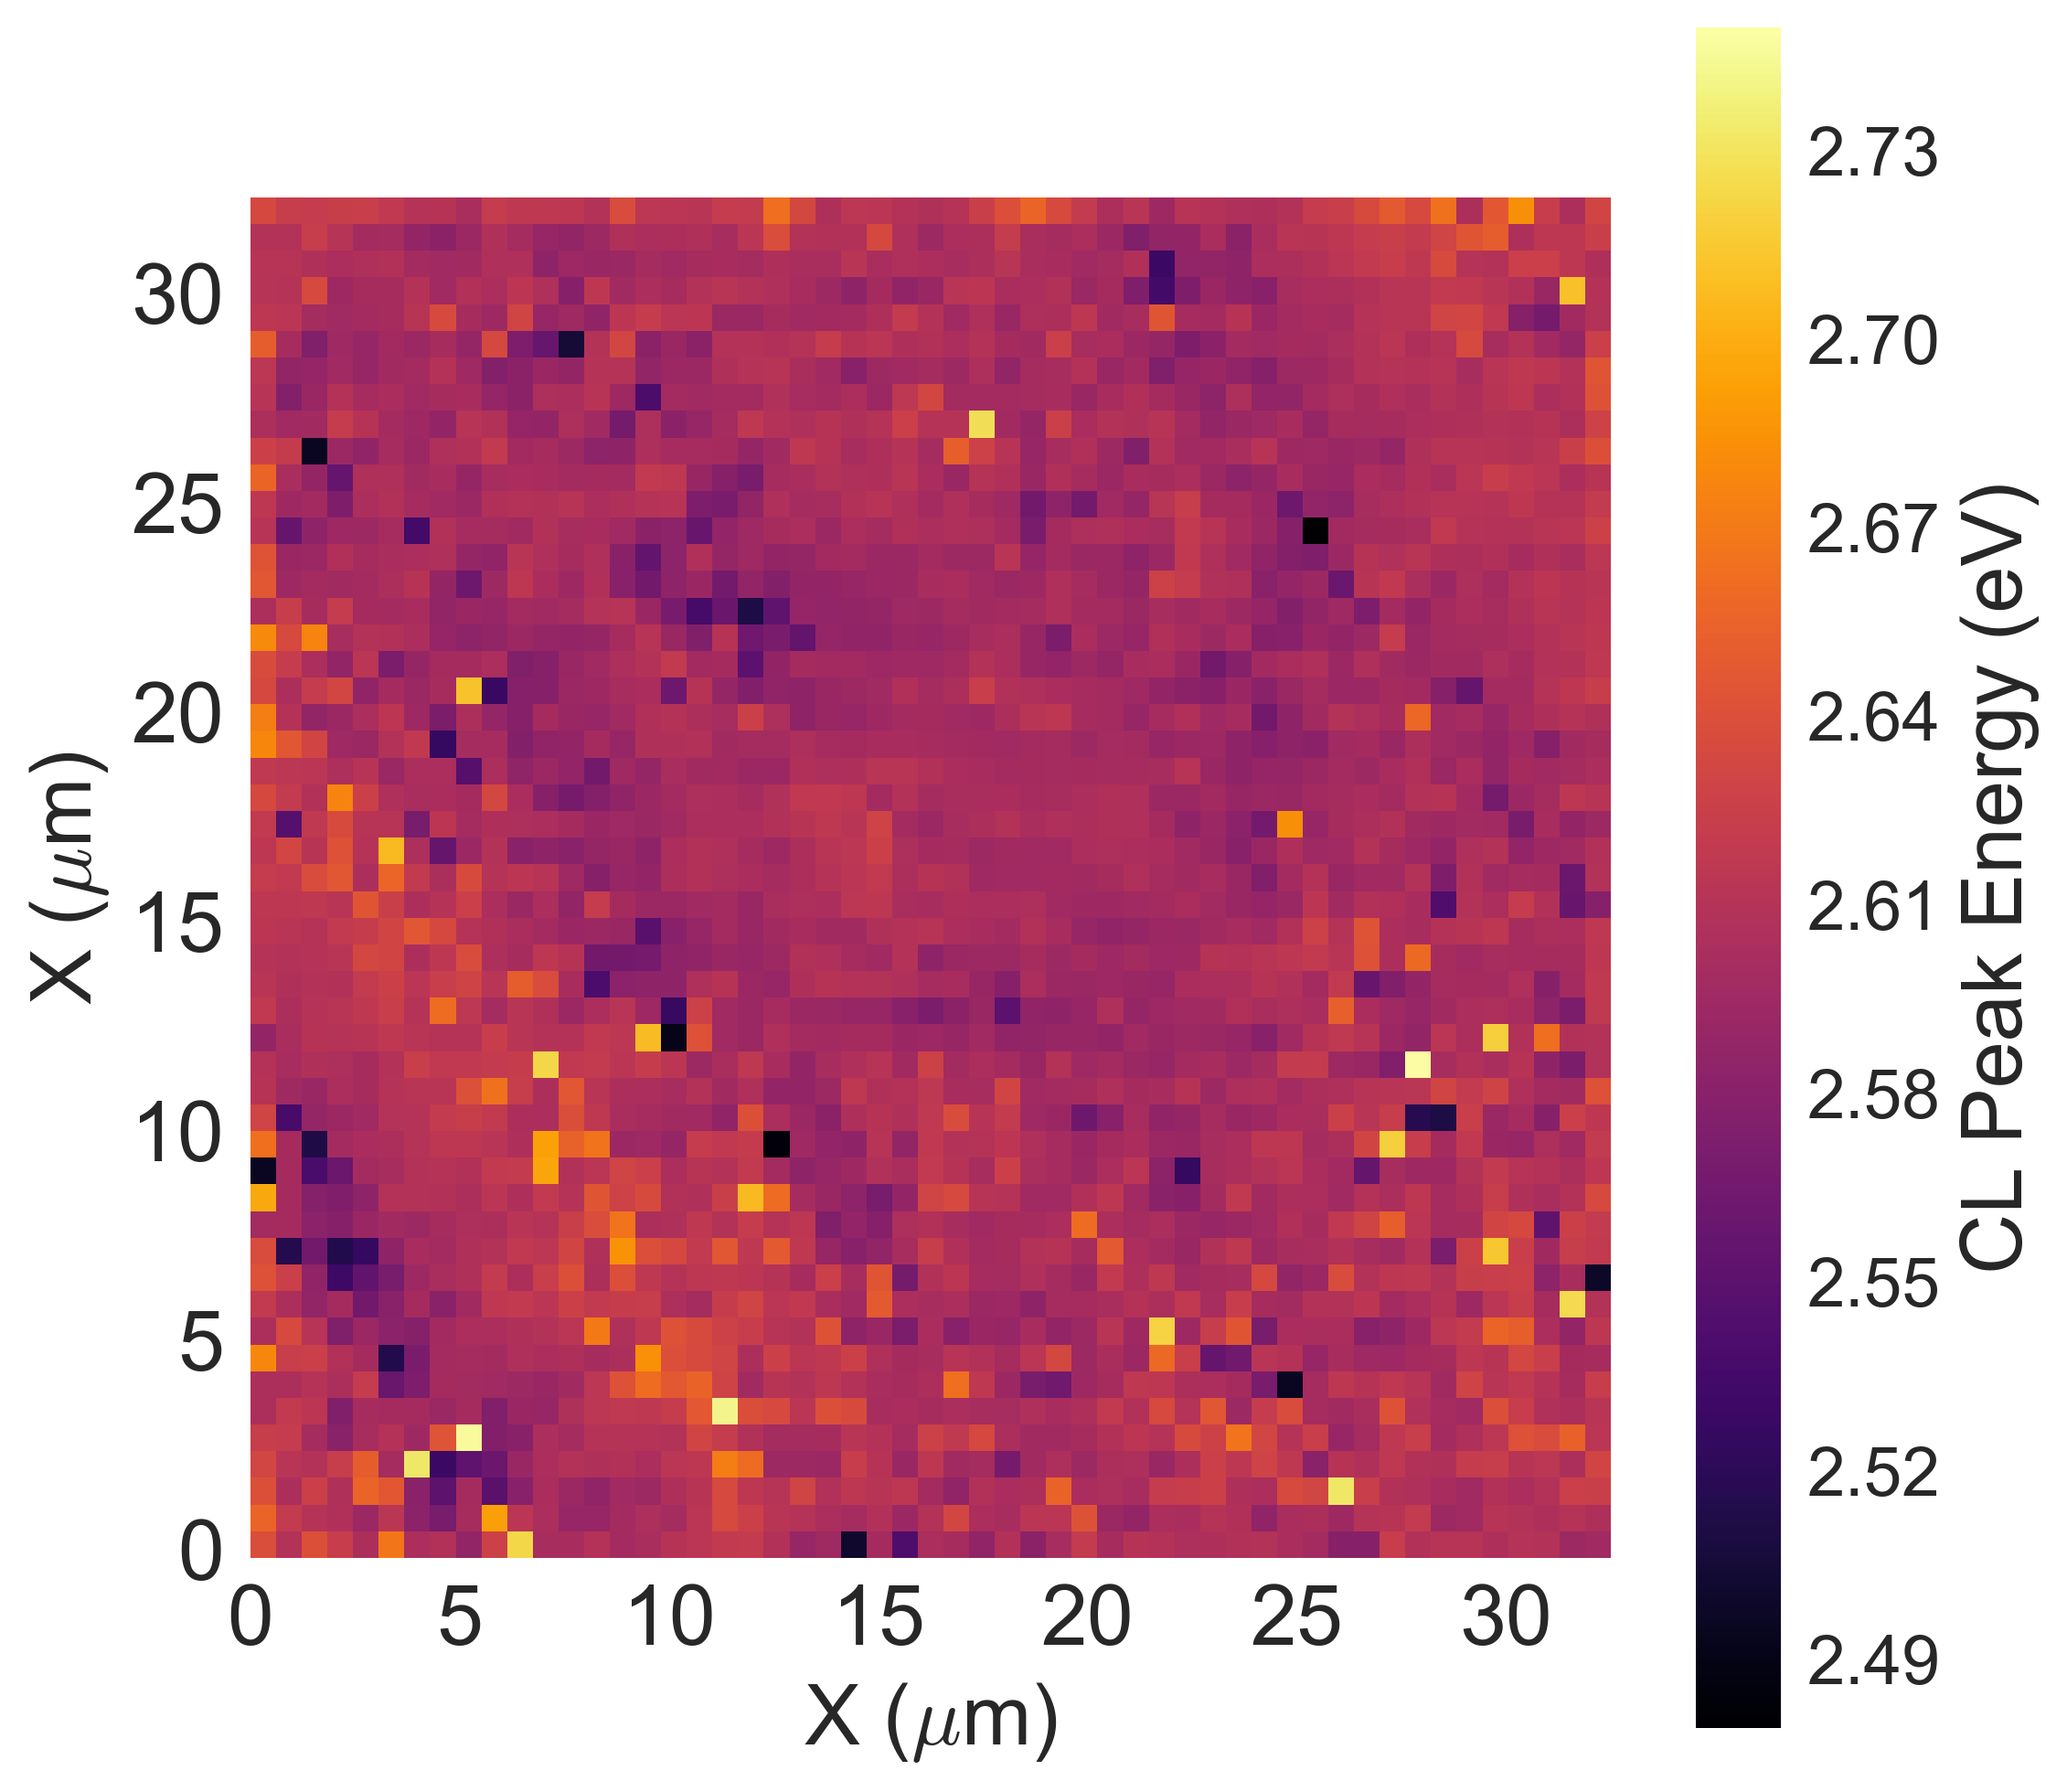
\includegraphics[width=1\linewidth]{Figs/Ch3/A-centre}
		\caption{}
	\end{subfigure}%
	
	\caption{a)CL peak intensity and b) CL peak energy for the feature shown in Fig.\ref{5610-SEM-CL}}
	\label{A-CL}
\end{figure}
\FloatBarrier

\begin{figure}[h]
	
	\begin{subfigure}[b]{0.48\textwidth}
		\centering
		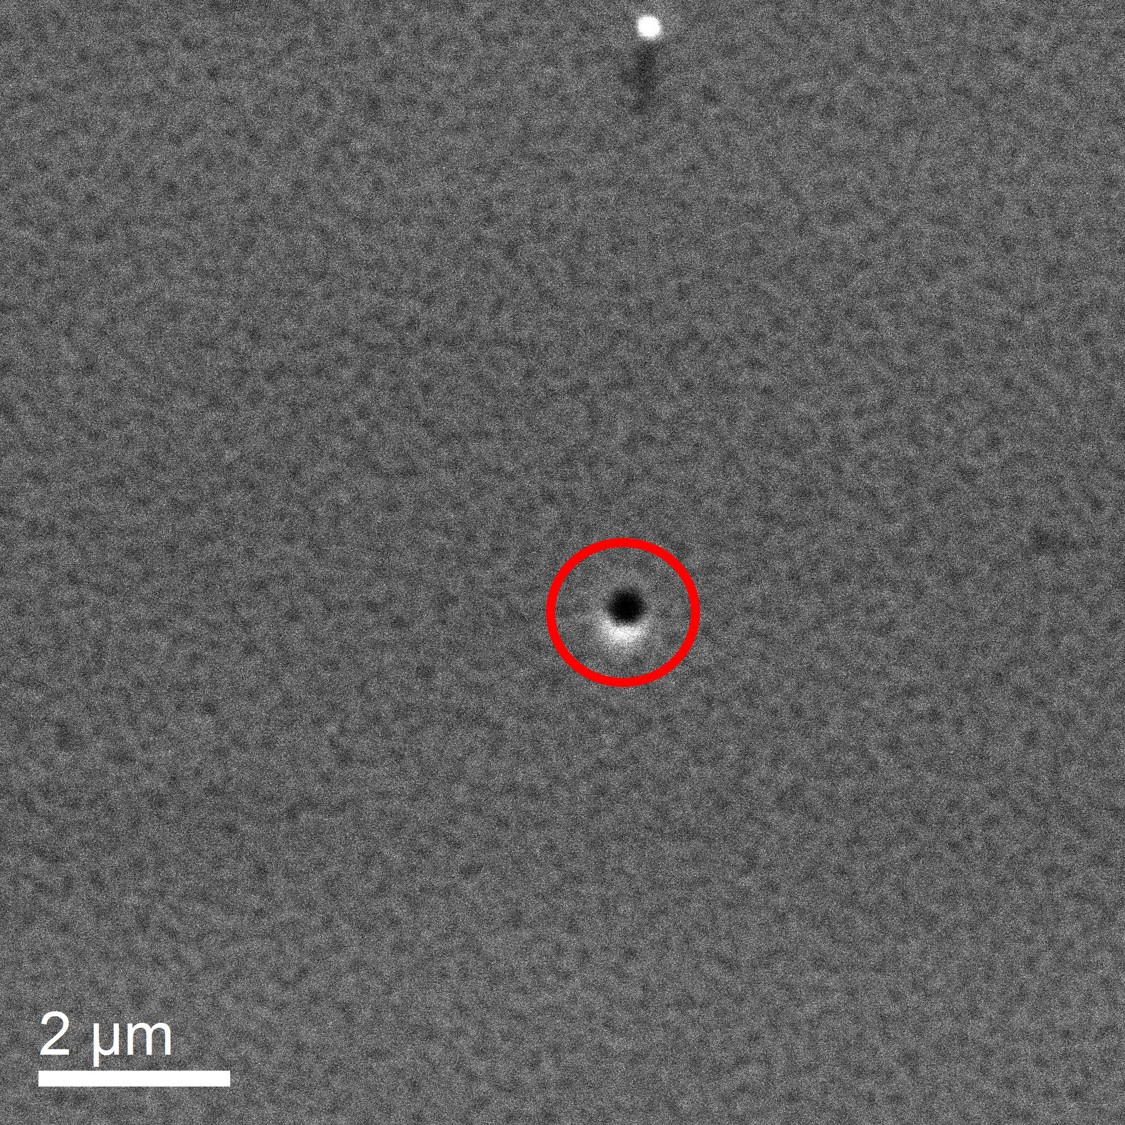
\includegraphics[width=0.7\linewidth]{Figs/Ch3/5608sem}
		\caption{}
		
	\end{subfigure}%
	\hspace*{0.5cm}
	\begin{subfigure}[b]{0.48\textwidth}
		\centering
		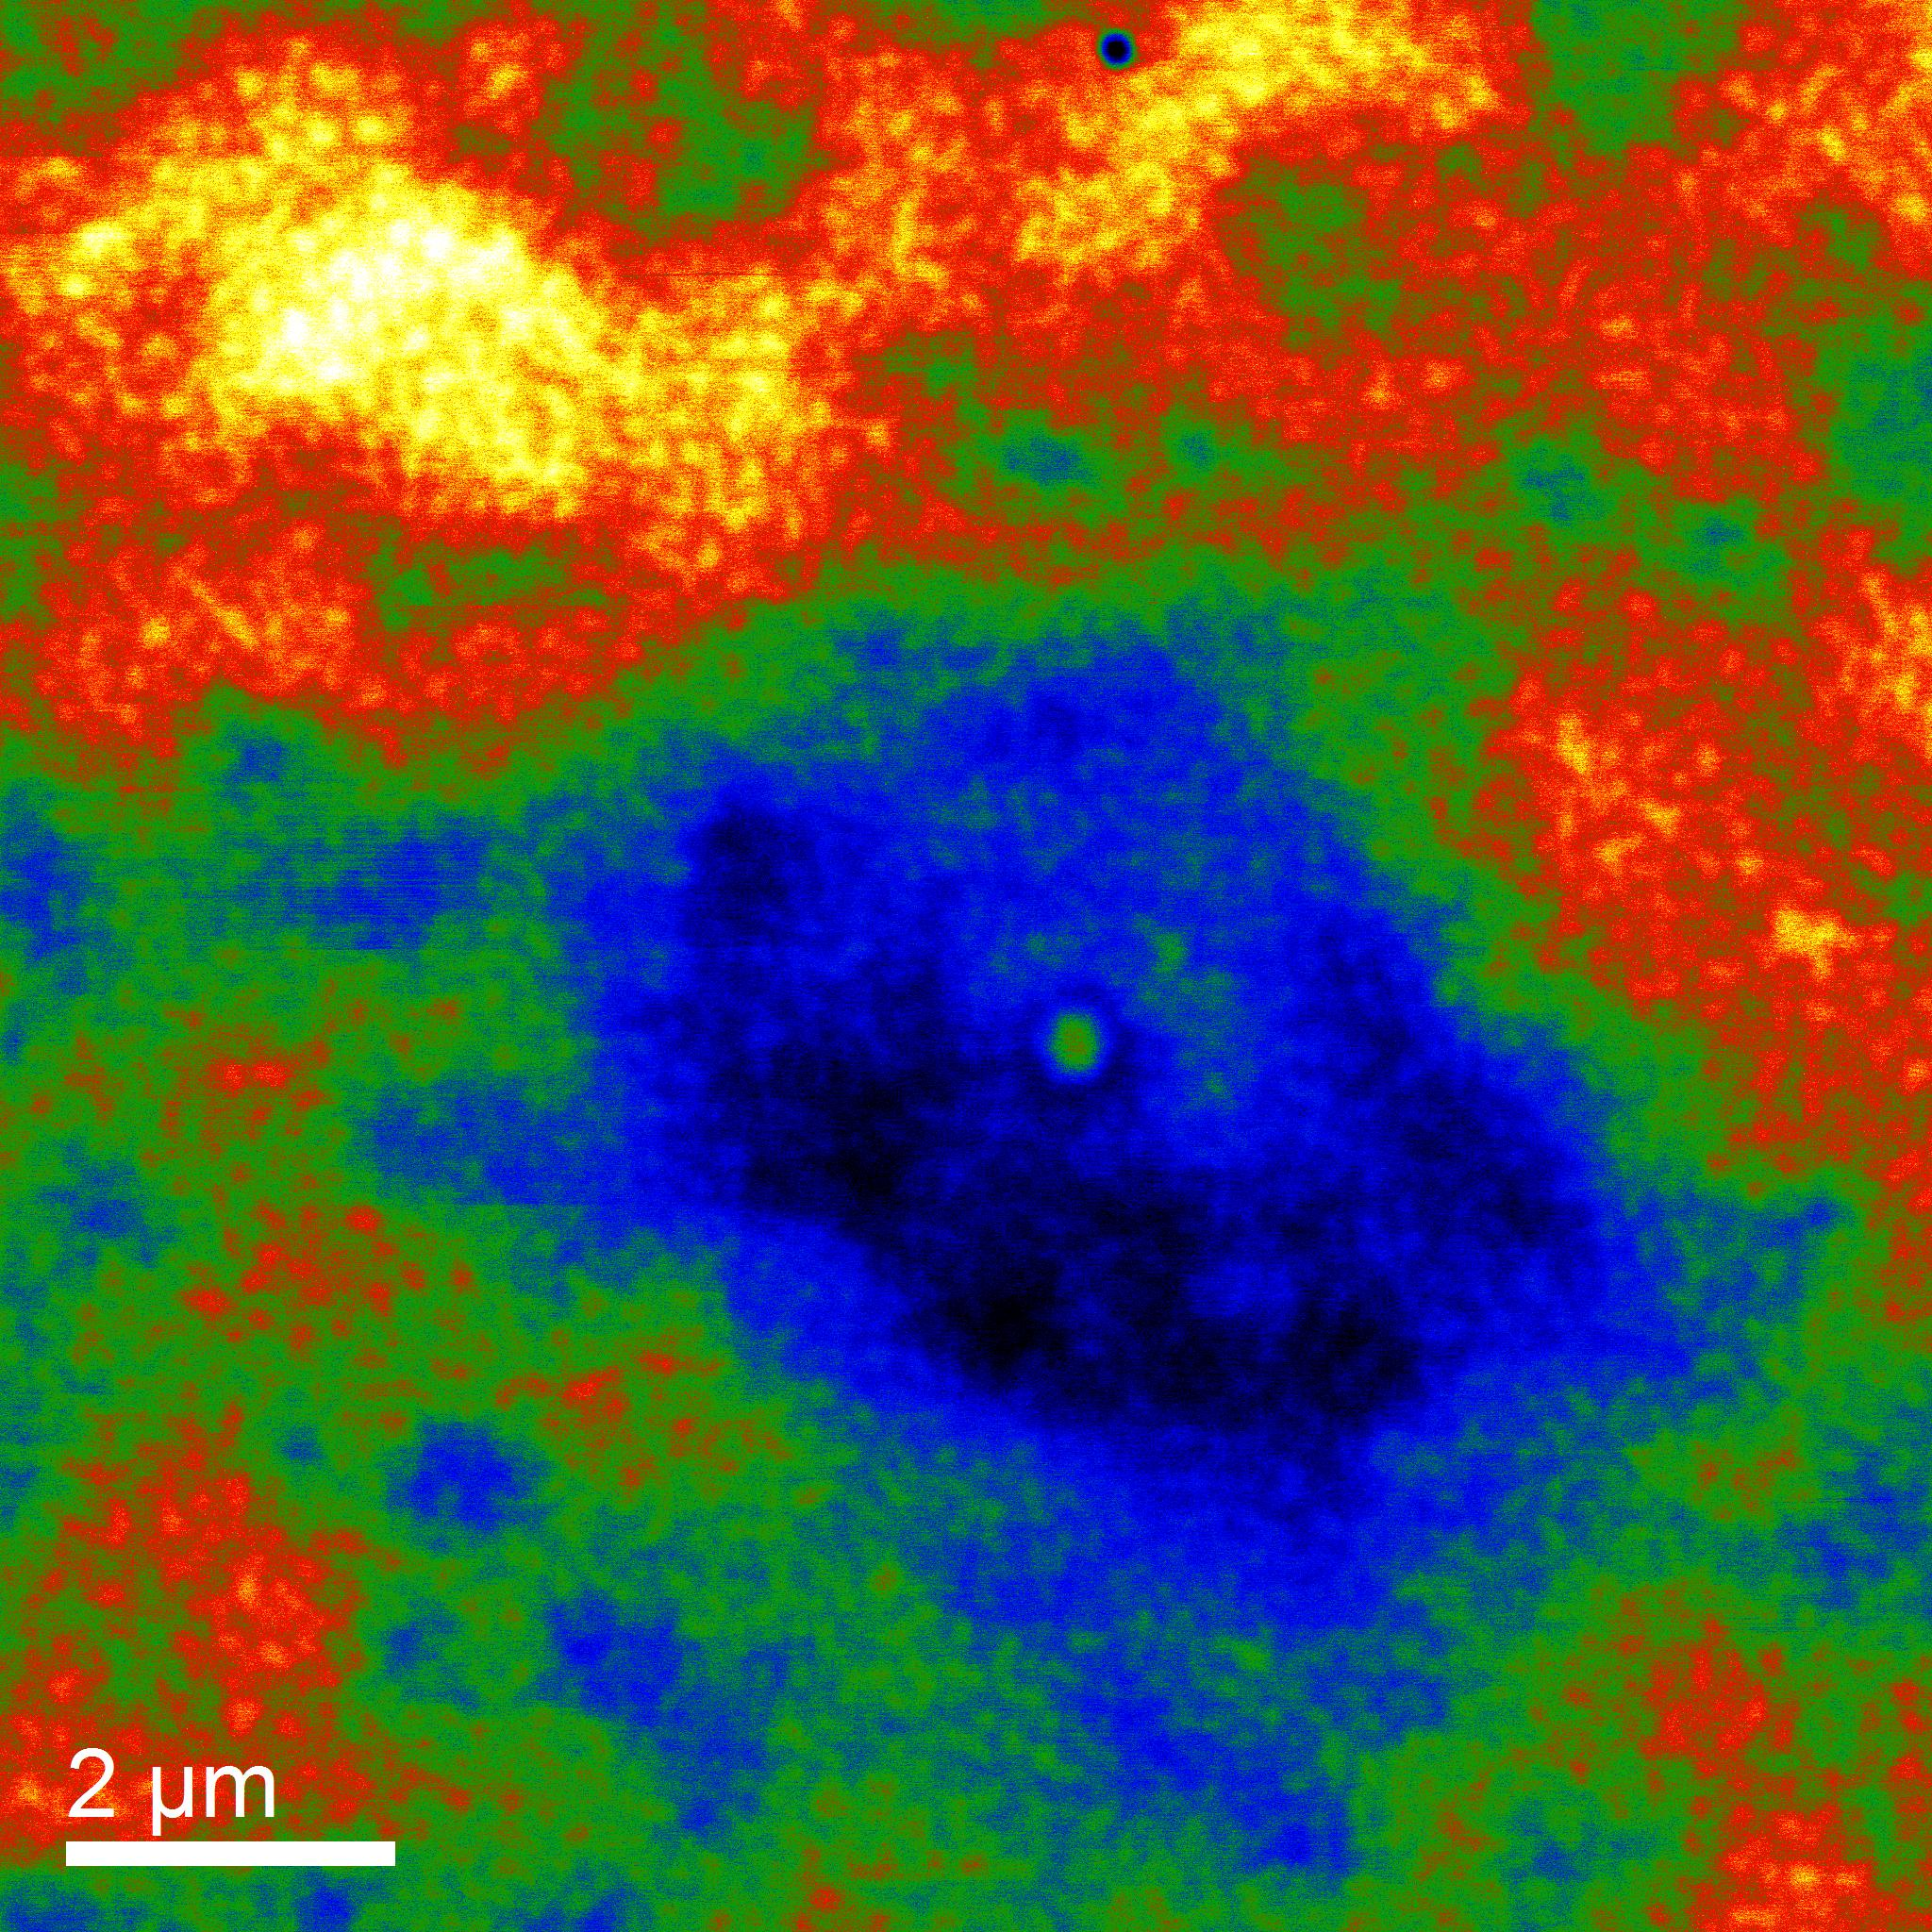
\includegraphics[width=0.7\linewidth]{Figs/Ch3/5608panCL}
		\caption{}
	\end{subfigure}%
	
	\caption{a) SEM micrograph and b) pan-CL image of an inhomogeneity in C5610A. The pan-CL image utilises a temperature scale (blue = low, red = high).}
	\label{5608-SEM-CL}
\end{figure}
\FloatBarrier

\begin{figure}[h]
	
	\begin{subfigure}[b]{0.48\textwidth}
		\centering
		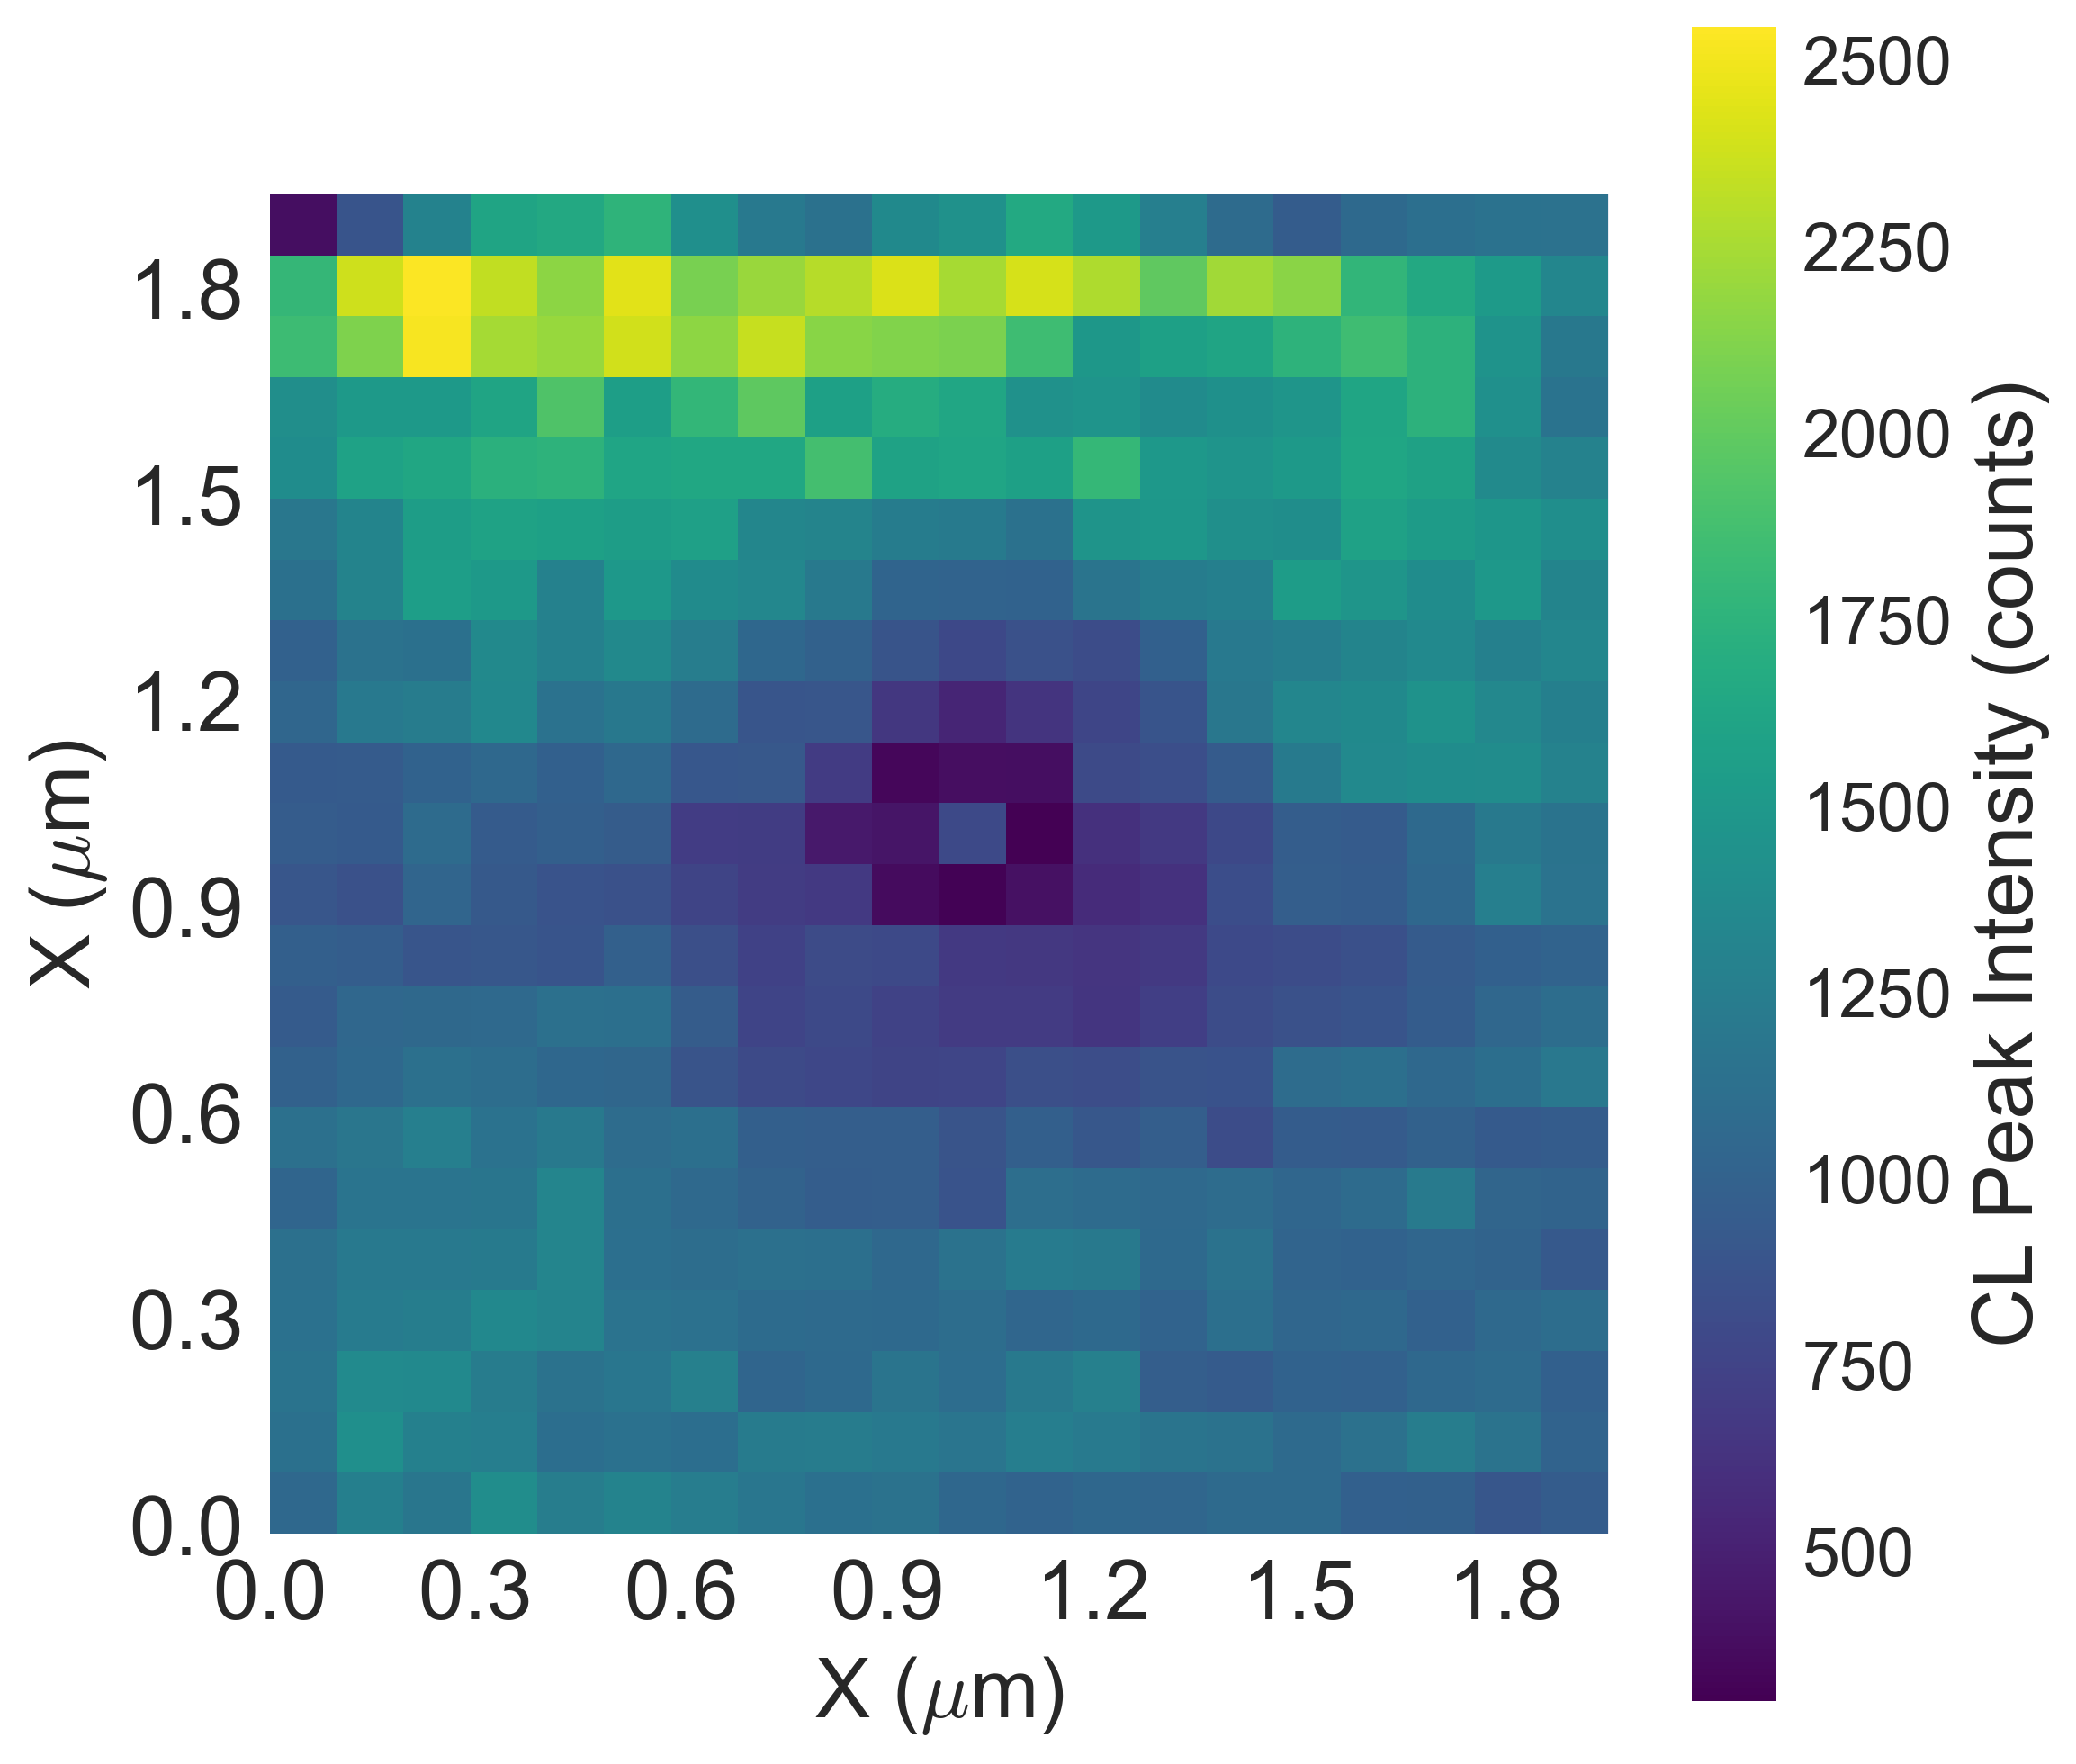
\includegraphics[width=1\linewidth]{Figs/Ch3/11-peak}
		\caption{}
		
	\end{subfigure}%
	\hspace*{0.5cm}
	\begin{subfigure}[b]{0.48\textwidth}
		\centering
		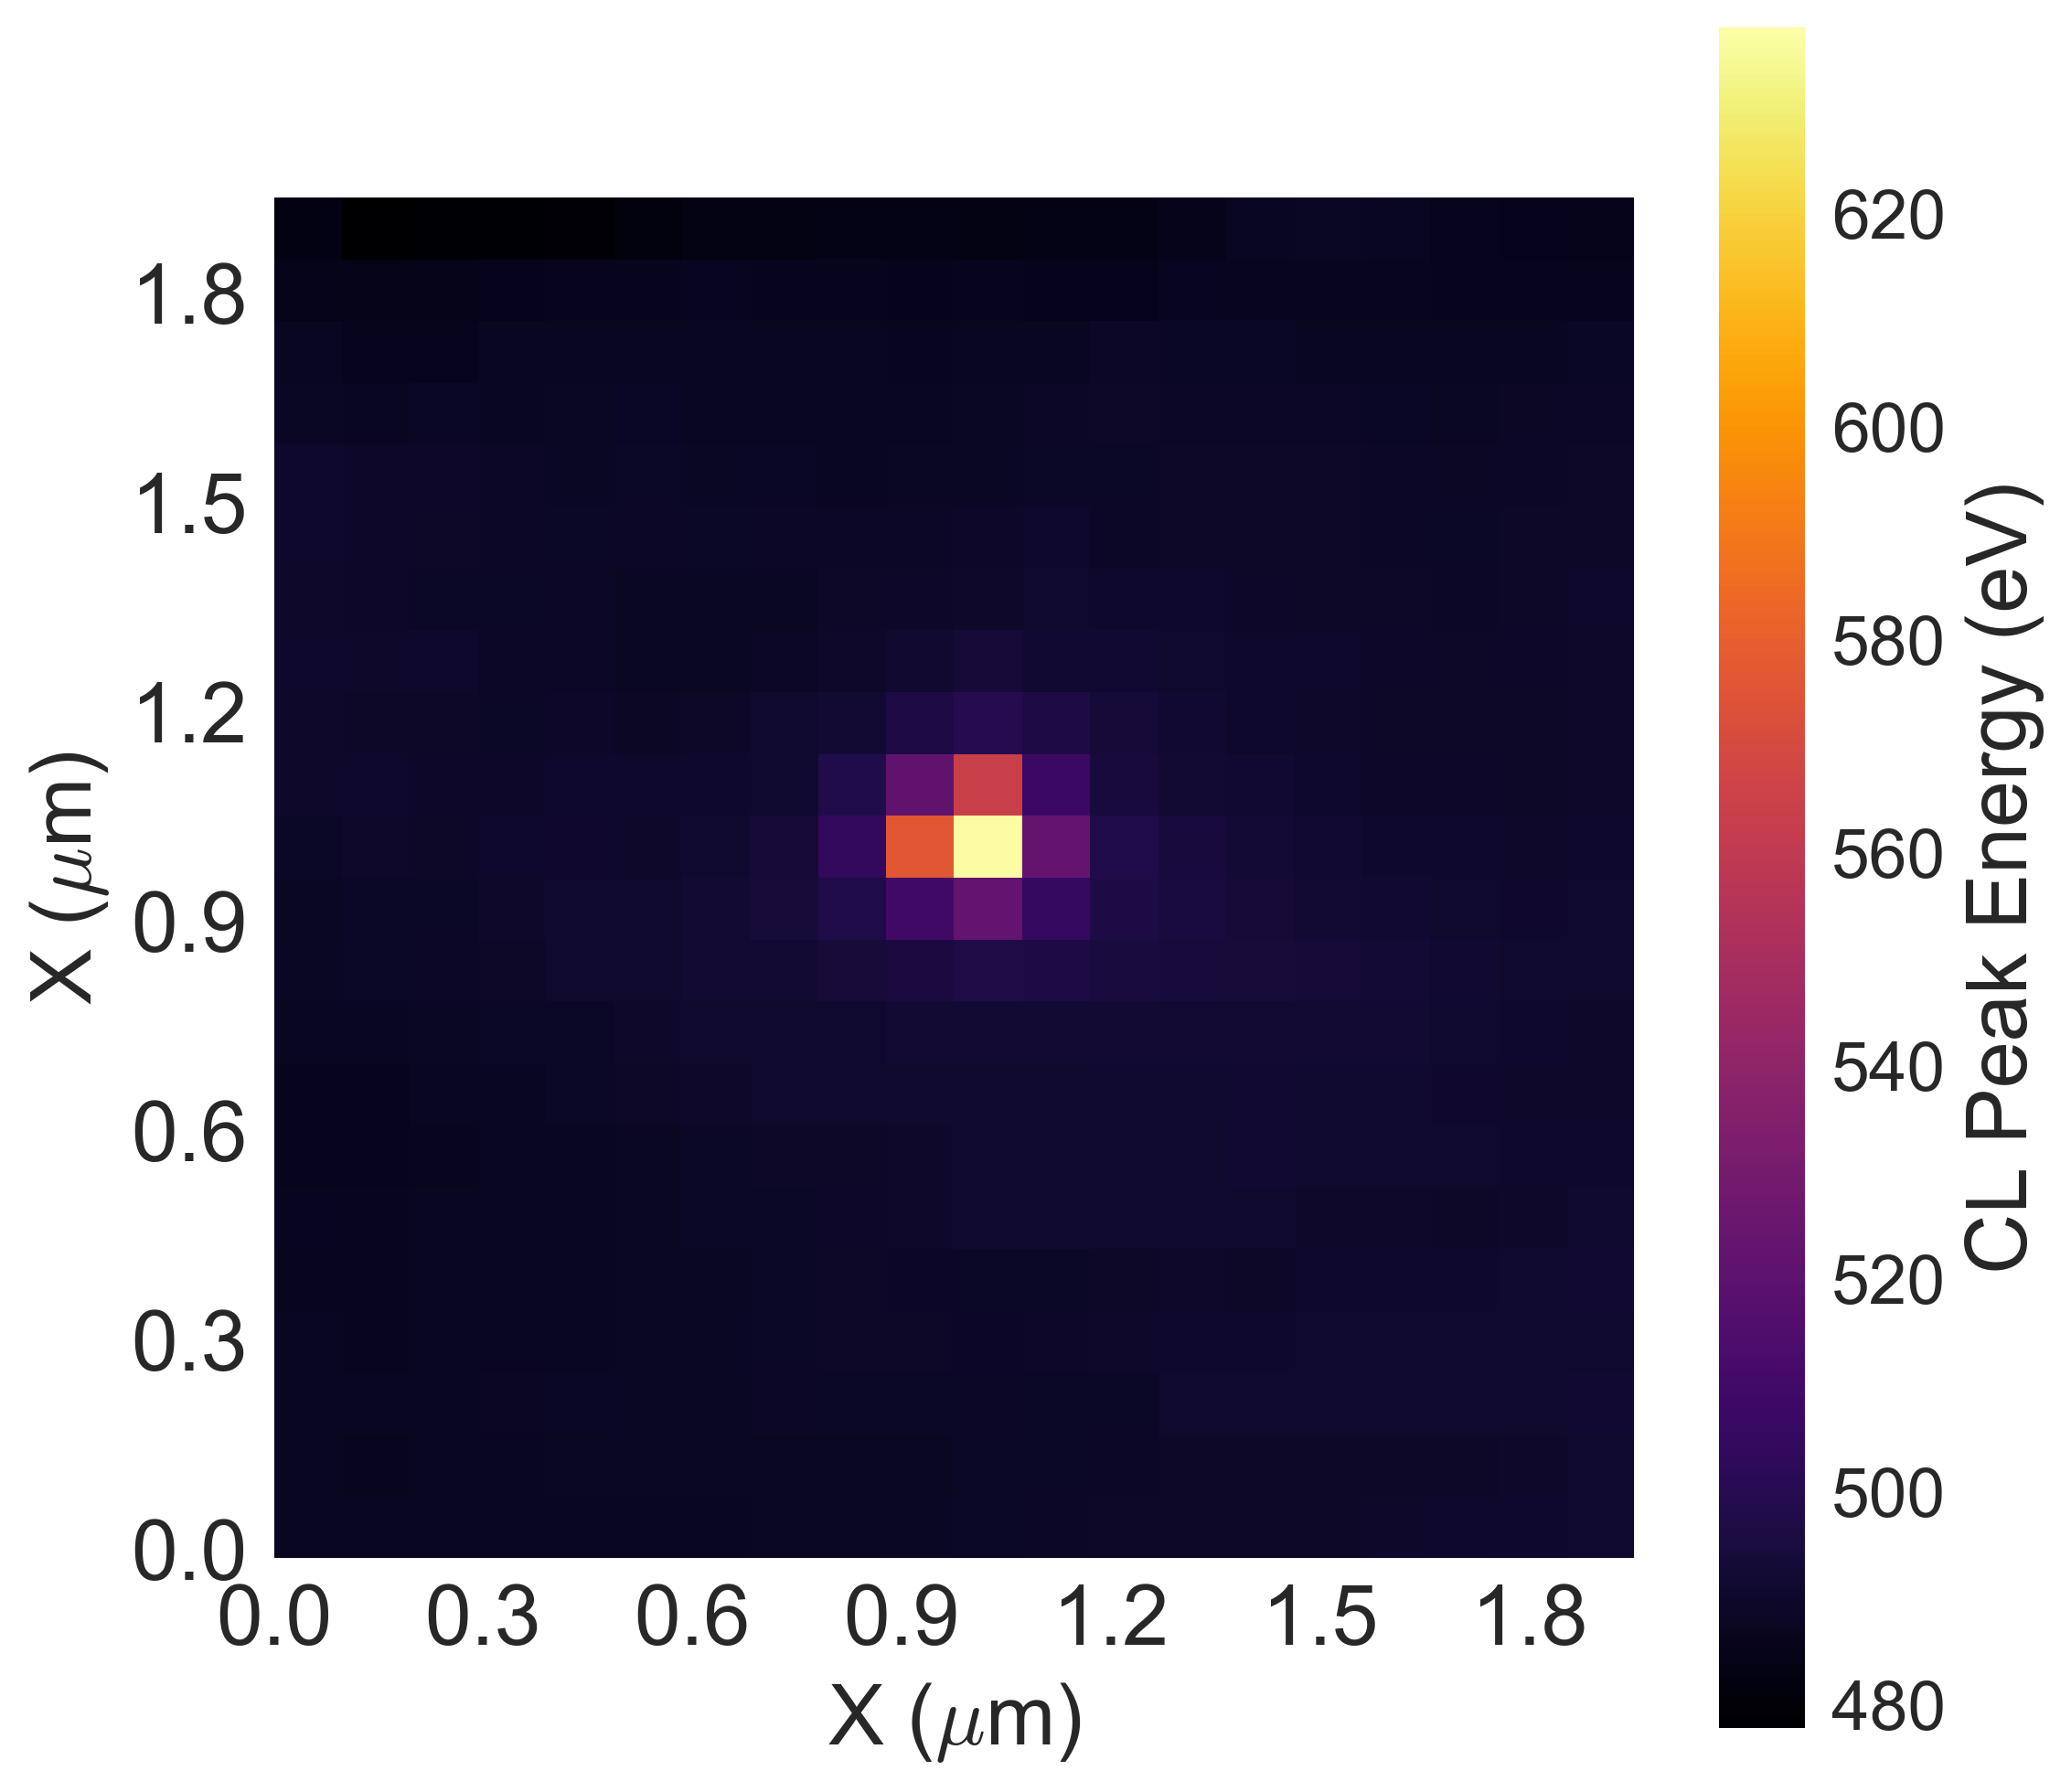
\includegraphics[width=1\linewidth]{Figs/Ch3/11-centre}
		\caption{}
	\end{subfigure}%
	
	\caption{a)CL peak intensity and b) CL peak energy for the feature shown in Fig.\ref{5608-SEM-CL}}
	\label{11-CL}
\end{figure}
\FloatBarrier
\subsection{Hexagonal Defect Analysis}

\subsection{Scanning Electron Microscopy}

\subsection{Atomic Force Microscopy}
AFM images of pits + C-AFM
\subsubsection{Conductive-AFM}

\subsection{TEM Lamella preparation}

\subsection{Scanning Transmission Electron Microscopy}
\subsubsection{Hexagonal Defect Morphology}
\subsubsection{Compositional Analysis}

\section{Simulations}

\section{Conclusion}

\section{Future Work}

